% Options for packages loaded elsewhere
\PassOptionsToPackage{unicode}{hyperref}
\PassOptionsToPackage{hyphens}{url}
\PassOptionsToPackage{dvipsnames,svgnames,x11names}{xcolor}
%
\documentclass[
  letterpaper,
  DIV=11,
  numbers=noendperiod]{scrreprt}

\usepackage{amsmath,amssymb}
\usepackage{iftex}
\ifPDFTeX
  \usepackage[T1]{fontenc}
  \usepackage[utf8]{inputenc}
  \usepackage{textcomp} % provide euro and other symbols
\else % if luatex or xetex
  \usepackage{unicode-math}
  \defaultfontfeatures{Scale=MatchLowercase}
  \defaultfontfeatures[\rmfamily]{Ligatures=TeX,Scale=1}
\fi
\usepackage{lmodern}
\ifPDFTeX\else  
    % xetex/luatex font selection
\fi
% Use upquote if available, for straight quotes in verbatim environments
\IfFileExists{upquote.sty}{\usepackage{upquote}}{}
\IfFileExists{microtype.sty}{% use microtype if available
  \usepackage[]{microtype}
  \UseMicrotypeSet[protrusion]{basicmath} % disable protrusion for tt fonts
}{}
\makeatletter
\@ifundefined{KOMAClassName}{% if non-KOMA class
  \IfFileExists{parskip.sty}{%
    \usepackage{parskip}
  }{% else
    \setlength{\parindent}{0pt}
    \setlength{\parskip}{6pt plus 2pt minus 1pt}}
}{% if KOMA class
  \KOMAoptions{parskip=half}}
\makeatother
\usepackage{xcolor}
\setlength{\emergencystretch}{3em} % prevent overfull lines
\setcounter{secnumdepth}{5}
% Make \paragraph and \subparagraph free-standing
\makeatletter
\ifx\paragraph\undefined\else
  \let\oldparagraph\paragraph
  \renewcommand{\paragraph}{
    \@ifstar
      \xxxParagraphStar
      \xxxParagraphNoStar
  }
  \newcommand{\xxxParagraphStar}[1]{\oldparagraph*{#1}\mbox{}}
  \newcommand{\xxxParagraphNoStar}[1]{\oldparagraph{#1}\mbox{}}
\fi
\ifx\subparagraph\undefined\else
  \let\oldsubparagraph\subparagraph
  \renewcommand{\subparagraph}{
    \@ifstar
      \xxxSubParagraphStar
      \xxxSubParagraphNoStar
  }
  \newcommand{\xxxSubParagraphStar}[1]{\oldsubparagraph*{#1}\mbox{}}
  \newcommand{\xxxSubParagraphNoStar}[1]{\oldsubparagraph{#1}\mbox{}}
\fi
\makeatother

\usepackage{color}
\usepackage{fancyvrb}
\newcommand{\VerbBar}{|}
\newcommand{\VERB}{\Verb[commandchars=\\\{\}]}
\DefineVerbatimEnvironment{Highlighting}{Verbatim}{commandchars=\\\{\}}
% Add ',fontsize=\small' for more characters per line
\usepackage{framed}
\definecolor{shadecolor}{RGB}{241,243,245}
\newenvironment{Shaded}{\begin{snugshade}}{\end{snugshade}}
\newcommand{\AlertTok}[1]{\textcolor[rgb]{0.68,0.00,0.00}{#1}}
\newcommand{\AnnotationTok}[1]{\textcolor[rgb]{0.37,0.37,0.37}{#1}}
\newcommand{\AttributeTok}[1]{\textcolor[rgb]{0.40,0.45,0.13}{#1}}
\newcommand{\BaseNTok}[1]{\textcolor[rgb]{0.68,0.00,0.00}{#1}}
\newcommand{\BuiltInTok}[1]{\textcolor[rgb]{0.00,0.23,0.31}{#1}}
\newcommand{\CharTok}[1]{\textcolor[rgb]{0.13,0.47,0.30}{#1}}
\newcommand{\CommentTok}[1]{\textcolor[rgb]{0.37,0.37,0.37}{#1}}
\newcommand{\CommentVarTok}[1]{\textcolor[rgb]{0.37,0.37,0.37}{\textit{#1}}}
\newcommand{\ConstantTok}[1]{\textcolor[rgb]{0.56,0.35,0.01}{#1}}
\newcommand{\ControlFlowTok}[1]{\textcolor[rgb]{0.00,0.23,0.31}{\textbf{#1}}}
\newcommand{\DataTypeTok}[1]{\textcolor[rgb]{0.68,0.00,0.00}{#1}}
\newcommand{\DecValTok}[1]{\textcolor[rgb]{0.68,0.00,0.00}{#1}}
\newcommand{\DocumentationTok}[1]{\textcolor[rgb]{0.37,0.37,0.37}{\textit{#1}}}
\newcommand{\ErrorTok}[1]{\textcolor[rgb]{0.68,0.00,0.00}{#1}}
\newcommand{\ExtensionTok}[1]{\textcolor[rgb]{0.00,0.23,0.31}{#1}}
\newcommand{\FloatTok}[1]{\textcolor[rgb]{0.68,0.00,0.00}{#1}}
\newcommand{\FunctionTok}[1]{\textcolor[rgb]{0.28,0.35,0.67}{#1}}
\newcommand{\ImportTok}[1]{\textcolor[rgb]{0.00,0.46,0.62}{#1}}
\newcommand{\InformationTok}[1]{\textcolor[rgb]{0.37,0.37,0.37}{#1}}
\newcommand{\KeywordTok}[1]{\textcolor[rgb]{0.00,0.23,0.31}{\textbf{#1}}}
\newcommand{\NormalTok}[1]{\textcolor[rgb]{0.00,0.23,0.31}{#1}}
\newcommand{\OperatorTok}[1]{\textcolor[rgb]{0.37,0.37,0.37}{#1}}
\newcommand{\OtherTok}[1]{\textcolor[rgb]{0.00,0.23,0.31}{#1}}
\newcommand{\PreprocessorTok}[1]{\textcolor[rgb]{0.68,0.00,0.00}{#1}}
\newcommand{\RegionMarkerTok}[1]{\textcolor[rgb]{0.00,0.23,0.31}{#1}}
\newcommand{\SpecialCharTok}[1]{\textcolor[rgb]{0.37,0.37,0.37}{#1}}
\newcommand{\SpecialStringTok}[1]{\textcolor[rgb]{0.13,0.47,0.30}{#1}}
\newcommand{\StringTok}[1]{\textcolor[rgb]{0.13,0.47,0.30}{#1}}
\newcommand{\VariableTok}[1]{\textcolor[rgb]{0.07,0.07,0.07}{#1}}
\newcommand{\VerbatimStringTok}[1]{\textcolor[rgb]{0.13,0.47,0.30}{#1}}
\newcommand{\WarningTok}[1]{\textcolor[rgb]{0.37,0.37,0.37}{\textit{#1}}}

\providecommand{\tightlist}{%
  \setlength{\itemsep}{0pt}\setlength{\parskip}{0pt}}\usepackage{longtable,booktabs,array}
\usepackage{calc} % for calculating minipage widths
% Correct order of tables after \paragraph or \subparagraph
\usepackage{etoolbox}
\makeatletter
\patchcmd\longtable{\par}{\if@noskipsec\mbox{}\fi\par}{}{}
\makeatother
% Allow footnotes in longtable head/foot
\IfFileExists{footnotehyper.sty}{\usepackage{footnotehyper}}{\usepackage{footnote}}
\makesavenoteenv{longtable}
\usepackage{graphicx}
\makeatletter
\newsavebox\pandoc@box
\newcommand*\pandocbounded[1]{% scales image to fit in text height/width
  \sbox\pandoc@box{#1}%
  \Gscale@div\@tempa{\textheight}{\dimexpr\ht\pandoc@box+\dp\pandoc@box\relax}%
  \Gscale@div\@tempb{\linewidth}{\wd\pandoc@box}%
  \ifdim\@tempb\p@<\@tempa\p@\let\@tempa\@tempb\fi% select the smaller of both
  \ifdim\@tempa\p@<\p@\scalebox{\@tempa}{\usebox\pandoc@box}%
  \else\usebox{\pandoc@box}%
  \fi%
}
% Set default figure placement to htbp
\def\fps@figure{htbp}
\makeatother

\newcommand{\Exg}{\operatorname{\mathbb{E}}} 
\newcommand{\Ex}{\mathbb{E}} 
\newcommand{\Ind}{\mathbb{I}}
\newcommand{\Var}{\operatorname{Var}}
\newcommand{\Cov}{\operatorname{Cov}}
\newcommand{\Corr}{\operatorname{Corr}}
\newcommand{\ee}{\mathrm{e}}
\usepackage{comment}
\KOMAoption{captions}{tableheading}
\makeatletter
\@ifpackageloaded{bookmark}{}{\usepackage{bookmark}}
\makeatother
\makeatletter
\@ifpackageloaded{caption}{}{\usepackage{caption}}
\AtBeginDocument{%
\ifdefined\contentsname
  \renewcommand*\contentsname{Table of contents}
\else
  \newcommand\contentsname{Table of contents}
\fi
\ifdefined\listfigurename
  \renewcommand*\listfigurename{List of Figures}
\else
  \newcommand\listfigurename{List of Figures}
\fi
\ifdefined\listtablename
  \renewcommand*\listtablename{List of Tables}
\else
  \newcommand\listtablename{List of Tables}
\fi
\ifdefined\figurename
  \renewcommand*\figurename{Figure}
\else
  \newcommand\figurename{Figure}
\fi
\ifdefined\tablename
  \renewcommand*\tablename{Table}
\else
  \newcommand\tablename{Table}
\fi
}
\@ifpackageloaded{float}{}{\usepackage{float}}
\floatstyle{ruled}
\@ifundefined{c@chapter}{\newfloat{codelisting}{h}{lop}}{\newfloat{codelisting}{h}{lop}[chapter]}
\floatname{codelisting}{Listing}
\newcommand*\listoflistings{\listof{codelisting}{List of Listings}}
\usepackage{amsthm}
\theoremstyle{plain}
\newtheorem{theorem}{Theorem}[chapter]
\theoremstyle{definition}
\newtheorem{definition}{Definition}[chapter]
\theoremstyle{definition}
\newtheorem{example}{Example}[chapter]
\theoremstyle{remark}
\AtBeginDocument{\renewcommand*{\proofname}{Proof}}
\newtheorem*{remark}{Remark}
\newtheorem*{solution}{Solution}
\newtheorem{refremark}{Remark}[chapter]
\newtheorem{refsolution}{Solution}[chapter]
\makeatother
\makeatletter
\makeatother
\makeatletter
\@ifpackageloaded{caption}{}{\usepackage{caption}}
\@ifpackageloaded{subcaption}{}{\usepackage{subcaption}}
\makeatother

\usepackage{bookmark}

\IfFileExists{xurl.sty}{\usepackage{xurl}}{} % add URL line breaks if available
\urlstyle{same} % disable monospaced font for URLs
\hypersetup{
  pdftitle={MATH5835M Statistical Computing},
  pdfauthor={Matthew Aldridge},
  colorlinks=true,
  linkcolor={blue},
  filecolor={Maroon},
  citecolor={Blue},
  urlcolor={Blue},
  pdfcreator={LaTeX via pandoc}}


\title{MATH5835M Statistical Computing}
\author{Matthew Aldridge}
\date{2025-09-30}

\begin{document}
\maketitle

\renewcommand*\contentsname{Table of contents}
{
\hypersetup{linkcolor=}
\setcounter{tocdepth}{2}
\tableofcontents
}

\bookmarksetup{startatroot}

\chapter*{About MATH5835}\label{about-math5835}
\addcontentsline{toc}{chapter}{About MATH5835}

\markboth{About MATH5835}{About MATH5835}

\section*{Organisation of MATH5835}\label{organisation-of-math5835}
\addcontentsline{toc}{section}{Organisation of MATH5835}

\markright{Organisation of MATH5835}

This module is \textbf{MATH5835M Statistical Computing}.

This module lasts for 11 weeks from 29 September to 12 December 2025.
The exam will take place sometime between 12 and 23 January 2026.

The module leader, the lecturer, and the main author of these notes is
\href{https://mpaldridge.github.io/}{Dr Matthew Aldridge}. (You can call
me ``Matt'', ``Matthew'', or ``Dr Aldridge'', pronounced
``\emph{old}-ridge''.) My email address is
\href{mailto:m.aldridge@leeds.ac.uk}{\nolinkurl{m.aldridge@leeds.ac.uk}},
although I much prefer questions in person at office hours (see below)
rather than by email.

The HTML webpage is the best way to view the course material. There is
also a \href{MATH5835M-Statistical-Computing.pdf}{\textbf{PDF version}},
although I have been much less careful about the presentation of this
material, and it does not include the problem sheets.

\subsection*{Lectures}\label{lectures}
\addcontentsline{toc}{subsection}{Lectures}

The main way you will learn new material for this module is by attending
lectures. There are three lectures per week:

\begin{itemize}
\item
  Mondays at 1400
\item
  Thursdays at 1200
\item
  Fridays at 1000
\end{itemize}

all in in
\href{https://students.leeds.ac.uk/buildings-and-rooms/3611/roger-stevens-lt-14-10m-14}{Roger
Stevens LT 14}.

I recommend taking your own notes during the lecture. I will put brief
summary notes from the lectures on this website, but they will not
reflect all the details I say out loud and write on the whiteboard.
Lectures will go through material quite quickly and the material may be
quite difficult, so it's likely you'll want to spend time reading
through your notes after the lecture. Lectures should be recorded on the
lecture capture system; I find it very difficult to read the whiteboard
in these videos, but if you unavoidably miss a lecture, for example due
to illness, you may find they are better than nothing.

In Weeks 3, 5, 7, 9 and 11, the Thursday lecture will operate as a
``problems class'' -- see more on this below.

Attendance at lectures in compulsory. You should record your attendance
using the UniLeeds app and the QR code on the wall in the 15 minutes
before the lecture or the 15 minutes after the lecture (but not during
the lecture).

\subsection*{Problem sheets and problem
classes}\label{problem-sheets-and-problem-classes}
\addcontentsline{toc}{subsection}{Problem sheets and problem classes}

Mathematics and statistics are ``doing'' subjects! To help you learn
material for the module and to help you prepare for the exam, I will
provide 5 unassessed problem sheets. These are for you to work through
in your own time to help you learn; they are \emph{not} formally
assessed. You are welcome to discuss work on the problem sheets with
colleagues and friends, although my recommendation would be to write-up
your ``last, best'' attempt neatly by yourself.

There will be an optional opportunity to submit one or two questions
from the problem sheet to me in advance of the problems class for some
brief informal feedback on your work. See the problem sheets for
details.

You should work through each problem sheet in preparation for the
problems class in the Thursday lecture of Week 3, 5, 7, 9 and 11. In the
problems class, you should be ready to explain your answers to questions
you managed to solve, discuss your progress on questions you partially
solved, and ask for help on questions you got stuck on.

You can also ask for extra help or feedback at office hours (see below).

\subsection*{Coursework}\label{coursework}
\addcontentsline{toc}{subsection}{Coursework}

There will be one piece of assessed coursework, which will make up 20\%
of your module mark. \hyperref[coursework]{You can read more about the
coursework here.}

The coursework will be in the form of a worksheet. The worksheet will
have some questions, mostly computational but also mathematical, and you
will have to write a report containing your answers and computations.

The assessed coursework will be introduced in the \textbf{computer
practical} sessions in Week 9.

The deadline for the coursework will be the penultimate day of the
Autumn term, \textbf{Thursday 12 December } at 1400. Feedback and marks
will be returned on Monday 13 January, the first day of the Spring term.

\subsection*{Office hours}\label{office-hours}
\addcontentsline{toc}{subsection}{Office hours}

I will run a n optional ``office hours'' drop-in session each week for
feedback and consultation. You can come along if you want to talk to me
about anything on the module, including if you'd like more feedback on
your attempts at problem sheet questions. (For extremely short queries,
you can approach me before or after lectures, but my response will often
be: ``Come to my office hours, and we can discuss it there!'')

Office hours will happen on \textbf{Thursdays from 1300 to 1400} -- so
directly after the Thursday lecture / problems class -- in my office,
which is \textbf{EC Stoner 9.10n} in ``Maths Research Deck'' area on the
9th floor of the EC Stoner building. (One way to the Maths Research Deck
is via the doors directly opposite the main entrance to the School of
Mathematics; you can also get there from Staircase 1 on the Level 10
``red route'' through EC Stoner, next to the Maths Satellite.) If you
cannot make this time, contact me for an alternative arrangement.

\subsection*{Exam}\label{exam}
\addcontentsline{toc}{subsection}{Exam}

There will be one exam, which will make up 80\% of your module mark.

The exam will be in the January 2026 exam period (12--23 January); the
date and time will be announced in December. The exam will be in person
and on campus.

The exam will last 2 hours and 30 minutes. The exam will consist of 4
questions, all compulsory. You will be allowed to use a permitted
calculator in the exam.

\section*{Content of MATH5835}\label{content-of-math5835}
\addcontentsline{toc}{section}{Content of MATH5835}

\markright{Content of MATH5835}

\subsection*{Necessary background}\label{necessary-background}
\addcontentsline{toc}{subsection}{Necessary background}

I recommend that students should have completed at least two
undergraduate level courses in probability or statistics -- although
confidence and proficiency in basic material is more important than very
deep knowledge of more complicated topics.

For Leeds undergraduates, MATH2715 Statistical Methods is an official
prerequisite (please get in touch with me if you are/were a Leeds
undergraduate and have not taken MATH2715), although confidence and
proficiency in the more basic material of MATH1710 \& MATH1712
Probability and Statistics 1 \& 2 is probably more important.

Some knowledge I will assume:

\begin{itemize}
\item
  \textbf{Probability:} Basic rules of probability; random variables,
  both continuous and discrete; ``famous'' distributions (especially the
  normal distribution and the continuous uniform distribution);
  expectation, variance, covariance, correlation; law of large numbers
  and central limit theorem.
\item
  \textbf{Statistics:} Estimation of parameters; bias and error; sample
  mean and sample variance
\end{itemize}

This module will also include an material on Markov chains. I won't
assume any pre-existing knowledge of this, and I will introduce all new
material we need, but students who have studied Markov chains before
(for example in the Leeds module MATH2750 Introduction to Markov
Processes) may find a couple of lectures here are merely a reminder of
things they already know.

The lectures will include examples using the \textbf{R} program
language. The coursework and problem sheets will require use of R. The
exam, while just a ``pencil and paper'' exam, will require understanding
and writing short portions of R code. We will assume basic R capability
-- that you can enter R commands, store R objects using the
\texttt{\textless{}-} assignment, and perform basic arithmetic with
numbers and vectors. Other concepts will be introduced as necessary. If
you want to use R on your own device, I recommend downloading (if you
have not already) the \href{https://cran.r-project.org}{R programming
language} and the \href{https://posit.co/downloads/}{program RStudio}.
(These lecture notes were written in R using RStudio.)

\subsection*{Syllabus}\label{syllabus}
\addcontentsline{toc}{subsection}{Syllabus}

We plan to cover the following topics in the module:

\begin{itemize}
\item
  \textbf{Monte Carlo estimation:} definition and examples; bias and
  error; variance reduction techniques: control variates, antithetic
  variables, importance sampling. {[}9 lectures{]}
\item
  \textbf{Random number generation:} pseudo-random number generation
  using linear congruential generators; inverse transform method;
  rejection sampling {[}7 lectures{]}
\item
  \textbf{Markov chain Monte Carlo} (MCMC)\textbf{:} {[}7 lectures{]}

  \begin{itemize}
  \item
    Introduction to Markov chains in discrete and continuous space
  \item
    Metropolis--Hastings algorithm: definition; examples; MCMC in
    practice; MCMC for Bayesian statistics
  \end{itemize}
\item
  \textbf{Resampling methods:} Empirical distribution; plug-in
  estimation; bootstrap statistics; bootstrap estimation {[}4
  lectures{]}
\item
  Frequently-asked questions {[}1 lecture{]}
\end{itemize}

Together with the 5 problems classes, this makes 33 lectures.

\subsection*{Book}\label{book}
\addcontentsline{toc}{subsection}{Book}

The following book is strongly recommended for the module:

\begin{itemize}
\tightlist
\item
  J Voss,
  \href{https://leeds.primo.exlibrisgroup.com/permalink/44LEE_INST/1fj430b/cdi_askewsholts_vlebooks_9781118728031}{\emph{An
  Introduction to Statistical Computing: A simulation-based approach}},
  Wiley Series in Computational Statistics, Wiley, 2014
\end{itemize}

The library has
\href{https://leeds.primo.exlibrisgroup.com/permalink/44LEE_INST/1fj430b/cdi_askewsholts_vlebooks_9781118728031}{electronic
access to this book} (and two paper copies).

Dr Voss is a lecturer in the School of Mathematics and the University of
Leeds, and has taught MATH5835 many times. \emph{An Introduction to
Statistical Computing} grew out of his lecture notes for this module, so
the book is ideally suited for this module. My lectures will follow this
book closely -- specifically:

\begin{itemize}
\item
  Monte Carlo estimation: Sections 3.1--3.3
\item
  Random number generation: Sections 1.1--1.4
\item
  Markov chain Monte Carlo: Section 2.3 and Sections 4.1--4.3
\item
  Bootstrap: Section 5.2
\end{itemize}

For a second look at material, for preparatory reading, for optional
extended reading, or for extra exercises, this book comes with my
highest recommendation!

\part{Monte Carlo estimation}

\chapter{Introduction to Monte Carlo}\label{introduction-to-monte-carlo}

\[ \]

Today, we'll start the first main topic of the module, which is called
``Monte Carlo estimation''. But first, a bit about the subject as a
whole.

\section{What is statistical
computing?}\label{what-is-statistical-computing}

``Statistical computing'' -- or ``computational statistics'' -- refers
to the branch of statistics that involves not attacking statistical
problems merely with a pencil and paper, but rather by combining human
ingenuity with the immense calculating powers of computers.

One of the big ideas here is \textbf{simulation}. Simulation is the idea
that we can understand the properties of a random model not by cleverly
working out the properties using theory -- this is usually impossible
for anything but the simplest ``toy models'' -- but rather by running
the model many times on a computer. From these many simulations, we can
observe and measure things like the typical (or ``expected'') behaviour,
the spread (or ``variance'') of the behaviour, and other things. This
concept of simulation is at the heart of the module MATH5835M
Statistical Computing.

In particular, we will look at \textbf{Monte Carlo} estimation. Monte
Carlo is about estimating a parameter, expectation or probability
related to a random variable by taking many samples of that random
variable, then computing a relevant sample mean from those samples. We
will study Monte Carlo in its standard ``basic'' form, then look at ways
we can make Monte Carlo estimation more accurate (Lectures 1--9).

To run a simulation -- for example, when performing Monte Carlo
estimation -- one needs random numbers with the correct distribution.
\textbf{Random number generation} (Lectures 10--16) will be an important
part of this module. We will look first at how to generate randomness of
any sort, and then how to manipulate that randomness into the shape of
the distributions we want.

Sometimes, it's not possible to generate perfectly independent samples
from exactly the distribution you want. But we can use the output of a
process called a ``Markov chain'' to get ``fairly independent'' samples
from nearly the distribution we want. When we perform Monte Carlo
estimation with the output of a Markov chain, this is called
\textbf{Markov chain Monte Carlo (MCMC)} (Lectures 17--23). MCMC has
become a vital part of modern Bayesian statistical analysis.

The final section of the module is about dealing with data. Choosing a
random piece of data from a given dataset is a lot like generating a
random number from a given distribution, and similar Monte Carlo
estimation ideas can be used to find out about that data. We think of a
dataset as being a sample from a population, and sampling again from
that dataset is known as \textbf{resampling} (Lecture 24--27). The most
important method of finding out about a population by using resampling
from a dataset is called the ``bootstrap'', and we will study the
bootstrap in detail.

MATH5835M Statistical Computing is a \emph{mathematics} module that will
concentrate on the \emph{mathematical} ideas that underpin statistical
computing. It is not a programming module that will go deeply into the
practical issues of the most efficient possible coding of the algorithms
we study. But we will want to investigate the behaviour of the methods
we learn about and to explore their properties, so will be computer
programming to help us do that. We will be using the statistical
programming language R, (although one could just as easily have used
Python or other similar languages). As my PhD supervisor often told me:
``You don't really understand a mathematical algorithm until you've
coded it up yourself.''

\section{What is Monte Carlo
estimation?}\label{what-is-monte-carlo-estimation}

Let \(X\) be a random variable. We recall the \textbf{expectation}
\(\Ex X\) of \(X\). If \(X\) is discrete with probability mass function
(PMF) \(p\), then the expectation of \(X\) is
\[ \Ex X = \sum_x x\,p(x) ;\] while if \(X\) is continuous with
probability density function (PDF) \(f\), then the expectation is
\[ \Ex X = \int_{-\infty}^{+\infty} x\,f(x)\,\mathrm{d}x . \] More
generally, the expectation of a function \(\phi\) of \(X\) is
\[ \Exg \phi(X) = \begin{cases} {\displaystyle \sum_x \phi(x)\,p(x)} & \text{for $X$ discrete}\\ {\displaystyle \int_{-\infty}^{+\infty} \phi(x)\,f(x)\,\mathrm{d}x}  & \text{for $X$ continuous.} \end{cases}\]
(This matches with the ``plain'' expectation when \(\phi(x) = x\).)

But how do we actually \emph{calculate} an expectation like one of
these? If \(X\) is discrete and can only take a small, finite number of
values, then we can simply add up the sum \(\sum_x \phi(x)\,p(x)\). But
otherwise, we just have to hope that \(\phi\) and \(p\) or \(f\) are
sufficiently ``nice'' that we can manage to work out the sum/integral
using a pencil and paper (and our brain). But while this is often
possible in the sort of ``toy example'' one comes across in maths or
statistics lectures, this is very rare in ``real life'' problems.

\textbf{Monte Carlo estimation} is the idea that we can get an
approximate answer for \(\Ex X\) or \(\Exg \phi(X)\) if we have access
to lots of samples from \(X\). If we have access to
\(X_1, X_2 \dots, X_n\) , independent and identically distributed (IID)
samples with the same distribution as \(X\), then we already know that
the mean
\[ \overline X = \frac{1}{n}(X_1 + X_2 + \cdots + X_n) = \frac{1}{n} \sum_{i=1}^n X_i \]
can be used to estimate the expectation \(\mathbb EX\). We know that
\(\overline X\) is usually close to the expectation \(\Ex X\), at least
if if the number of samples \(n\) is large; this is justified by the
``law of large numbers'', which says that \(\overline X \to \mathbb EX\)
as \(n \to \infty\).

Similarly, we can use
\[ \frac{1}{n} \big(\phi(X_1) + \phi(X_2) + \cdots + \phi(X_n) \big) = \frac{1}{n} \sum_{i=1}^n \phi(X_i) \]
to estimate \(\Exg \phi(X)\). The law of large numbers again says that
this estimate tends to the correct value \(\Exg \phi(X)\) as
\(n \to \infty\).

In this module we will write that \(X_1, X_2, \dots, X_n\) is a
``\textbf{random sample} from \(X\)'' to mean that
\(X_1, X_2, \dots, X_n\) are IID with the same distribution as \(X\).

\begin{definition}[]\protect\hypertarget{def-MCest}{}\label{def-MCest}

Let \(X\) be a random variable, \(\phi\) a function, and write
\(\theta = \Exg\phi(X)\). Then the \textbf{Monte Carlo estimator}
\(\widehat\theta_n^{\mathrm{MC}}\) of \(\theta\) is
\[ \widehat{\theta}_n^{\mathrm{MC}} = \frac{1}{n} \sum_{i=1}^n \phi(X_i) , \]
where \(X_1, X_2, \dots, X_n\) are a random sample from \(X\).

\end{definition}

While general ideas for estimating using simulation go back a long time,
the modern theory of Monte Carlo estimation was developed by the
physicists \href{https://en.wikipedia.org/wiki/Stanisław_Ulam}{Stanislaw
Ulam} and \href{https://en.wikipedia.org/wiki/John_von_Neumann}{John von
Neumann}. Ulam (who was Polish) and von Neumann (who was Hungarian)
moved to the US in the early 1940s to work on the Manhattan project to
build the atomic bomb (as made famous by the film \emph{Oppenheimer}).
Later in the 1940s, they worked together in the Los Alamos National
Laboratory continuing their research on nuclear physics generally and
nuclear weapons more specifically, where they used simulations on early
computers to help them numerically solve difficult mathematical and
physical problems.

The name ``Monte Carlo'' was chosen because the use of randomness to
solve such problems reminded them of gamblers in the casinos of Monte
Carlo, Monaco. Ulam and von Neumann also worked closely with another
colleague Nicholas Metropolis, whose work we will study later in this
module.

\section{Examples}\label{examples}

Let's see some simple examples of Monte Carlo estimation using R.

\begin{example}[]\protect\hypertarget{exm-MCexp}{}\label{exm-MCexp}

Let's suppose we've forgotten the expectation of the exponential
distribution \(X \sim \operatorname{Exp}(2)\) with rate 2. In this
simple case, we could work out the answer using the PDF
\(f(x) = 2\mathrm{e}^{-2x}\) as\\
\[ \mathbb E X = \int_0^\infty x\,2\mathrm{e}^{-2x}\,\mathrm{d}x \]and,
without too much difficulty, get the answer \(\frac12\). But instead,
let's do this the Monte Carlo way.

In R, we can use the \texttt{rexp()} function to get IID samples from
the exponential distribution: the full syntax is
\texttt{rexp(n,\ rate)}, which gives \texttt{n} samples from an
exponential distribution with rate \texttt{rate}. The following code
takes the mean of \(n = 100\) samples from the exponential distribution.

\begin{Shaded}
\begin{Highlighting}[]
\NormalTok{n }\OtherTok{\textless{}{-}} \DecValTok{100}
\NormalTok{samples }\OtherTok{\textless{}{-}} \FunctionTok{rexp}\NormalTok{(n, }\DecValTok{2}\NormalTok{)}
\NormalTok{MCest }\OtherTok{\textless{}{-}}\NormalTok{ (}\DecValTok{1} \SpecialCharTok{/}\NormalTok{ n) }\SpecialCharTok{*} \FunctionTok{sum}\NormalTok{(samples)}
\NormalTok{MCest}
\end{Highlighting}
\end{Shaded}

\begin{verbatim}
[1] 0.4594331
\end{verbatim}

So our Monte Carlo estimate is 0.4594, to 4 decimal places.

That's fairly close to the correct answer of \(\frac12\). But we should
(hopefully) be able to get a more accurate estimation if we use more
samples. We could also simplify the third line of our code by using the
\texttt{mean()} function.

\begin{Shaded}
\begin{Highlighting}[]
\NormalTok{n }\OtherTok{\textless{}{-}} \FloatTok{1e6}
\NormalTok{samples }\OtherTok{\textless{}{-}} \FunctionTok{rexp}\NormalTok{(n, }\DecValTok{2}\NormalTok{)}
\NormalTok{MCest }\OtherTok{\textless{}{-}} \FunctionTok{mean}\NormalTok{(samples)}
\NormalTok{MCest}
\end{Highlighting}
\end{Shaded}

\begin{verbatim}
[1] 0.4996347
\end{verbatim}

In the second line, \texttt{1e6} is R code for the scientific notation
\(1 \times 10^6\), or a million. I just picked this as ``a big number,
but where my code still only took a few seconds to run.''

Our new Monte Carlo estimate is 0.4996, which is (probably) much closer
to the true value of \(\frac12\).

\end{example}

By the way: all R code ``chunks'' displayed in the notes should work
perfectly if you copy-and-paste them into RStudio. (Indeed, when I
compile these lecture notes in RStudio, all the R code gets run on my
computer -- so I'm certain in must work correctly!) If you hover over a
code chunk, a little ``clipboard'' icon should appear in the top-right,
and clicking on that will copy it so you can paste it into RStudio. I
strongly encourage playing about with the code as a good way to learn
this material and explore further!

\begin{example}[]\protect\hypertarget{exm-MC2}{}\label{exm-MC2}

Let's try another example. Let \(X \sim \operatorname{N}(1, 2^2)\) be a
normal distribution with mean 1 and standard deviation 2. Suppose we
want to find out \(\mathbb E(\sin X)\) (for some reason). While it
\emph{might} be possible to somehow calculate the integral
\[ \mathbb E(\sin X) = \int_{-\infty}^{+\infty} (\sin x) \, \frac{1}{\sqrt{2\pi\times 2^2}} \exp\left(-\frac{(x - 1)^2}{2\times 2^2}\right) \, \mathrm{d} x , \]
that looks extremely difficult to me.

Instead, a Monte Carlo estimation of \(\mathbb{E}(\sin X)\) is very
straightforward: we just take the mean of the sine of a bunch of
normally distributed random numbers. That is we get a random samples
\(X_1, X_2, \dots, X_n\) from \(X\); then take the mean of the values
\[\sin(X_1), \sin(X_2), \dots, \sin(X_n) .\]

(We must remember, though, when using the \texttt{rnorm()} function to
generate normally distributed random variates, that the third argument
is the \emph{standard deviation}, here \(2\), \emph{not} the variance,
here \(2^2 = 4\).)

\begin{Shaded}
\begin{Highlighting}[]
\NormalTok{n }\OtherTok{\textless{}{-}} \FloatTok{1e6}
\NormalTok{samples }\OtherTok{\textless{}{-}} \FunctionTok{rnorm}\NormalTok{(n, }\DecValTok{1}\NormalTok{, }\DecValTok{2}\NormalTok{)}
\NormalTok{MCest }\OtherTok{\textless{}{-}} \FunctionTok{mean}\NormalTok{(}\FunctionTok{sin}\NormalTok{(samples))}
\NormalTok{MCest}
\end{Highlighting}
\end{Shaded}

\begin{verbatim}
[1] 0.1131249
\end{verbatim}

Our Monte Carlo estimate is 0.11312.

\end{example}

\textbf{Next time:} \emph{We look at more examples of things we can
estimate using the Monte Carlo method.}

\textbf{Summary:}

\begin{itemize}
\item
  Statistical computing is about solving statistical problems by
  combining human ingenuity with computing power.
\item
  The Monte Carlo estimate of \(\Exg \phi(X)\) is
  \[ \widehat{\theta}_n^{\mathrm{MC}} = \frac{1}{n} \sum_{i=1}^n \phi(X_i) , \]
  where \(X_1, \dots, X_n\) are IID random samples from \(X\).
\item
  Monte Carlo estimation typically gets more accurate as the number of
  samples \(n\) gets bigger.
\end{itemize}

\textbf{Read more:}
\href{https://leeds.primo.exlibrisgroup.com/permalink/44LEE_INST/1fj430b/cdi_askewsholts_vlebooks_9781118728031}{Voss,
\emph{An Introduction to Statistical Computing}}, Section 3.1 and
Subsection 3.2.1.

\chapter{Uses of Monte Carlo}\label{uses-of-monte-carlo}

\[ \]

Quick recap: Last time we defined the Monte Carlo estimator for an
expectation of a function of a random variable \(\theta = \Exg \phi(X)\)
to be
\[ \widehat{\theta}_n^{\mathrm{MC}} = \frac{1}{n} \big(\phi(X_1) + \phi(X_2) + \cdots + \phi(X_n) \big) = \frac{1}{n} \sum_{i=1}^n \phi(X_i) , \]
where \(X_1, X_2, \dots, X_n\) are independent random samples from
\(X\).

Today we look at two other things we can estimate using Monte Carlo
simulation: probabilities, and integrals.

\section{Monte Carlo for
probabilities}\label{monte-carlo-for-probabilities}

What if we want to find a \emph{probability}, rather than an
expectation? What if we want \(\mathbb P(X = x)\) for some \(x\), or
\(\mathbb P(X \geq a)\) for some \(a\), or, more generally,
\(\mathbb P(X \in A)\) for some set \(A\)?

The key thing that will help us here is the \emph{indicator function}.
The indicator function simply tells us whether an outcome \(x\) is in a
set \(A\) or not.

\begin{definition}[]\protect\hypertarget{def-indicator}{}\label{def-indicator}

Let \(A\) be a set. Then the \textbf{indicator function} \(\Ind_A\) is
defined by
\[ \Ind_A(x) = \begin{cases} 1 & \text{if $x \in A$} \\ 0 & \text{if $x \notin A$.} \end{cases} \]

\end{definition}

The set \(A\) could just be a single element \(A = \{y\}\). In that case
\(\Ind_A(x)\) is 1 if \(x = y\) and 0 if \(x \neq y\). Or \(A\) could be
a semi-infinite interval, like \(A = [a, \infty)\). In that case
\(\Ind_A(x)\) is 1 if \(x \geq a\) and 0 if \(x < a\).

Why is this helpful? Well \(\Ind_A\) is a function, so let's think about
what the expectation \(\Exg \Ind_A(X)\) would be for some random
variable \(X\). Since \(\Ind_A\) can only take two values, 0 and 1, we
have \begin{align*}
\Exg \Ind_A(X) &= \sum_{y \in\{0,1\}} y\,\mathbb P\big( \Ind_A(X) = y \big) \\\
  &= 0 \times \mathbb P\big( \Ind_A(X) = 0 \big) + 1 \times \mathbb P\big( \Ind_A(X) = 1 \big) \\
  &= 0 \times \mathbb P(X \notin A) + 1 \times \mathbb P(X \in A) \\
  &= \mathbb P(X \in A) .
\end{align*} P(X \in A) . \textbackslash end\{align*\} In line three, we
used that \(\Ind_A(X) = 0\) if and only if \(X \notin A\), and that
\(\Ind_A(X) = 1\) if and only if \(X \in A\).

So the expectation of an indicator function a set is the probability
that \(X\) is in that set. This idea connects ``expectations of
functions'' back to probabilities: if we want to find
\(\mathbb P(X \in A)\) we can find the expectation of \(\Ind_A(X)\).

With this idea in hand, how do we estimate
\(\theta = \mathbb P(X \in A)\) using the Monte Carlo method? We write
\(\theta = \Exg\Ind_A(X)\). Then our Monte Carlo estimator is
\[  \widehat{\theta}_n^{\mathrm{MC}} = \frac{1}{n} \sum_{i=1}^n \Ind_A(X_i) . \]

We remember that \(\Ind_A(X_i)\) is 1 if \(X_i \in A\) and 0 otherwise.
So if we add up \(n\) of these, we count an extra +1 each time we have
an \(X_i \in A\). So \(\sum_{i=1}^n \Ind_A(X_i)\) counts the total
number of the \(X_i\) that are in \(A\). So the Monte Carlo estimator
can be written as
\[  \widehat{\theta}_n^{\mathrm{MC}} = \frac{\# \text{ of } X_i \text{ that are in $A$}}{n} . \]
(I'm using \(\#\) as shorthand for ``the number of''.)

Although we've had to do a bit of work to get here, this a totally
logical outcome! The right-hand side here is the proportion of the
samples for which \(X_i \in A\). And if we want to estimate the
probability something happens, looking at the proportion of times it
happens in a random sample is very much the ``intuitive'' estimate to
take. And that intuitive estimate is indeed the Monte Carlo estimate!

\begin{example}[]\protect\hypertarget{exm-MCprob}{}\label{exm-MCprob}

\emph{Let} \(Z \sim \operatorname{N}(0,1)\) \emph{be a standard normal
distribution. Estimate} \(\mathbb P(Z > 2)\)\emph{.}

This is a question that it is impossible to answer exactly using a
pencil and paper: there's no closed form for
\[ \mathbb P(Z > 2) = \int_2^\infty \frac{1}{\sqrt{2\pi}}\,\mathrm{e}^{-z^2/2}\,\mathrm{d}z , \]
so we'll have to use an estimation method.

The Monte Carlo estimate means taking a random sample
\(Z_1, Z_2, \dots, Z_n\) of standard normals, and calculating what
proportion of them are greater than 2. In R, we can do this as follows.

\begin{Shaded}
\begin{Highlighting}[]
\NormalTok{n }\OtherTok{\textless{}{-}} \FloatTok{1e6}
\NormalTok{samples }\OtherTok{\textless{}{-}} \FunctionTok{rnorm}\NormalTok{(n)}
\NormalTok{MCest }\OtherTok{\textless{}{-}} \FunctionTok{mean}\NormalTok{(samples }\SpecialCharTok{\textgreater{}} \DecValTok{2}\NormalTok{)}
\NormalTok{MCest}
\end{Highlighting}
\end{Shaded}

\begin{verbatim}
[1] 0.022716
\end{verbatim}

In the second line, we could have written \texttt{rnorm(n,\ 0,\ 1)}.
But, if you don't give the parameters \texttt{mean} and \texttt{sd} to
the function \texttt{rnorm()}, R just assumes you want the standard
normal with \texttt{mean\ =\ 0} and \texttt{sd\ =\ 1}.

We can check our answer: R's inbuilt \texttt{pnorm()} function estimates
probabilities for the normal distribution (using a method that, in this
specific case, is much quicker and more accurate than Monte Carlo
estimation). The true answer is very close to

\begin{Shaded}
\begin{Highlighting}[]
\FunctionTok{pnorm}\NormalTok{(}\DecValTok{2}\NormalTok{, }\AttributeTok{lower.tail =} \ConstantTok{FALSE}\NormalTok{)}
\end{Highlighting}
\end{Shaded}

\begin{verbatim}
[1] 0.02275013
\end{verbatim}

so our estimate was pretty good.

\end{example}

We should explain the third line in the code we used for the Monte Carlo
estimation \texttt{mean(samples\ \textgreater{}\ 2)}. In R, some
statements can be answered ``true'' or ``false'': these are often
statements involving equality \texttt{==} (that's a \emph{double} equals
sign) or inequalities like \texttt{\textless{}}, \texttt{\textless{}=},
\texttt{\textgreater{}=}, \texttt{\textgreater{}}, for example. So
\texttt{5\ \textgreater{}\ 2} is \texttt{TRUE} but \texttt{3\ ==\ 7} is
\texttt{FALSE}. These can be applied ``component by component'' to
vectors. So, for example, testing which numbers from 1 to 10 are greater
than or equal to 7, we get

\begin{Shaded}
\begin{Highlighting}[]
\DecValTok{1}\SpecialCharTok{:}\DecValTok{10} \SpecialCharTok{\textgreater{}=} \DecValTok{7}
\end{Highlighting}
\end{Shaded}

\begin{verbatim}
 [1] FALSE FALSE FALSE FALSE FALSE FALSE  TRUE  TRUE  TRUE  TRUE
\end{verbatim}

six \texttt{FALSE}s (for 1 to 6) followed by four \texttt{TRUE}s (for 7
to 10).

We can also use \texttt{\&} (``and'') and \texttt{\textbar{}} (``or'')
in true/false statements like these.

But R also knows to treat \texttt{TRUE} like the number 1 and
\texttt{FALSE} like the number 0. (This is just like the concept of the
indicator function we've been discussing.) So if we add up some
\texttt{TRUE}s and \texttt{FALSE}s, R simply counts how many
\texttt{TRUE}s there are

\begin{Shaded}
\begin{Highlighting}[]
\FunctionTok{sum}\NormalTok{(}\DecValTok{1}\SpecialCharTok{:}\DecValTok{10} \SpecialCharTok{\textgreater{}=} \DecValTok{7}\NormalTok{)}
\end{Highlighting}
\end{Shaded}

\begin{verbatim}
[1] 4
\end{verbatim}

So in our Monte Carlo estimation code,
\texttt{samples\ \textgreater{}\ 2} was a vector of \texttt{TRUE}s and
\texttt{FALSE}s, depending on whether each sample was greater than 2 or
not, then \texttt{mean(samples\ \textgreater{}\ 2)} took the
\emph{proportion} of the samples that were greater than 2.

\section{Monte Carlo for integrals}\label{monte-carlo-for-integrals}

There's another thing -- a non-statistics thing -- that Monte Carlo
estimation is useful for. We can use Monte Carlo estimation to
approximate integrals that are too hard to do by hand.

This might seem surprising. Estimating the expectation of (a function
of) a random variable seems a naturally statistical thing to do. But an
integral is just a straight maths problem -- there's not any randomness
at all. But actually, integrals and expectations are very similar
things.

Let's think of an integral: say, \[ \int_a^b h(x) \,\mathrm{d}x ,\] the
integral of some function \(h\) (the ``integrand'') between the limits
\(a\) and \(b\). Now let's compare that to the integral \(\Exg \phi(X)\)
of a continuous random variable that we can estimate using Monte Carlo
estimation,
\[ \Exg \phi(X) = \int_{-\infty}^\infty \phi(x)\,f(x)\, \mathrm{d} x. \]
Matching things up, we can see that we if we were to a function \(\phi\)
and a PDF \(f\) such that
\begin{equation}\phantomsection\label{eq-match}{ \phi(x)\,f(x) = \begin{cases} 0 & x < a \\ h(x) & a \leq x \leq b \\ 0 & x > b , \end{cases} }\end{equation}
then we would have
\[ \Exg \phi(X) = \int_{-\infty}^\infty \phi(x)\,f(x)\, \mathrm{d} x = \int_a^b h(x) \,\mathrm{d}x, \]
so the value of the expectation would be precisely the value of the
integral we're after. Then we could use Monte Carlo to estimate that
expectation/integral.

There are lots of choices of \(\phi\) and \(f\) that would satisfy this
the condition in Equation~\ref{eq-match}. But a ``common-sense'' choice
that often works is to pick \(f\) to be the PDF of \(X\), a continuous
uniform distribution on the interval \([a,b]\). (This certainly works
when \(a\) and \(b\) are finite, anyway.) Recall that the continuous
uniform distribution means that \(X\) has PDF
\[ f(x) = \begin{cases} 0 & x < a \\ \displaystyle{\frac{1}{b-a}} & a \leq x \leq b \\ 0 & x > b . \end{cases} \]
Comparing this equation with Equation~\ref{eq-match}, we then have to
choose \[\phi(x) = \frac{h(x)}{f(x)} = (b-a)h(x).\]

Putting this all together, we have
\[ \Exg \phi(X) = \int_{-\infty}^{+\infty} \phi(x)\,f(x)\,\mathrm{d}x = \int_a^b (b-a)h(x)\,\frac{1}{b-a}\,\mathrm{d}x = \int_a^b h(x) \,\mathrm{d}x ,\]
as required. This can then be estimated using the Monte Carlo method.

\begin{definition}[]\protect\hypertarget{def-MCint}{}\label{def-MCint}

Consider an integral \(\theta = \int_a^b h(x)\,\mathrm{d}x\). Let \(f\)
be the probability density function of a random variable \(X\) and let
\(\phi\) be function such that Equation~\ref{eq-match} holds. Then the
\textbf{Monte Carlo estimator} \(\widehat\theta_n^{\mathrm{MC}}\) of the
integral \(\theta\) is
\[ \widehat{\theta}_n^{\mathrm{MC}} = \frac{1}{n} \sum_{i=1}^n \phi(X_i) , \]
where \(X_1, X_2, \dots, X_n\) are a random sample from \(X\).

\end{definition}

\begin{example}[]\protect\hypertarget{exm-MCint}{}\label{exm-MCint}

Suppose we want to approximate the integral
\[ \int_0^2 x^{1.6} (2-x)^{0.7} \, \mathrm{d}x . \]

Since this is an integral on the finite interval \([0,2]\), it would
seem to make sense to pick \(X\) to be uniform on \([0,2]\). This means
we should take
\[\phi(x) = \frac{h(x)}{f(x)} = (2-0)h(x) = 2\,x^{1.6}(2-x)^{0.7}.\] We
can then approximate this integral in R using the Monte Carlo estimator
\[ \int_0^2 x^{1.6} (2-x)^{0.7} \, \mathrm{d}x = \operatorname{\mathbb{E}} \phi(X) \approx \frac{1}{n} \sum_{i=1}^n 2\,X_i^{1.6} (2-X_i)^{0.7} . \]

\begin{Shaded}
\begin{Highlighting}[]
\NormalTok{n }\OtherTok{\textless{}{-}} \FloatTok{1e6}
\NormalTok{integrand }\OtherTok{\textless{}{-}} \ControlFlowTok{function}\NormalTok{(x) x}\SpecialCharTok{\^{}}\FloatTok{1.6} \SpecialCharTok{*}\NormalTok{ (}\DecValTok{2} \SpecialCharTok{{-}}\NormalTok{ x)}\SpecialCharTok{\^{}}\FloatTok{0.7}
\NormalTok{a }\OtherTok{\textless{}{-}} \DecValTok{0}
\NormalTok{b }\OtherTok{\textless{}{-}} \DecValTok{2}
\NormalTok{samples }\OtherTok{\textless{}{-}} \FunctionTok{runif}\NormalTok{(n, a, b)}
\FunctionTok{mean}\NormalTok{((b }\SpecialCharTok{{-}}\NormalTok{ a) }\SpecialCharTok{*} \FunctionTok{integrand}\NormalTok{(samples))}
\end{Highlighting}
\end{Shaded}

\begin{verbatim}
[1] 1.444437
\end{verbatim}

You have perhaps noticed that, here and elsewhere, I tend to split my R
code up into lots of small bits, perhaps slightly unnecessarily. After
all, those 6 lines of code could simply have been written as just 2
lines

\begin{Shaded}
\begin{Highlighting}[]
\NormalTok{samples }\OtherTok{\textless{}{-}} \FunctionTok{runif}\NormalTok{(}\FloatTok{1e6}\NormalTok{, }\DecValTok{0}\NormalTok{, }\DecValTok{2}\NormalTok{)}
\FunctionTok{mean}\NormalTok{(}\DecValTok{2} \SpecialCharTok{*}\NormalTok{ samples}\SpecialCharTok{\^{}}\FloatTok{1.6} \SpecialCharTok{*}\NormalTok{ (}\DecValTok{2} \SpecialCharTok{{-}}\NormalTok{ samples)}\SpecialCharTok{\^{}}\FloatTok{0.7}\NormalTok{)}
\end{Highlighting}
\end{Shaded}

There's nothing \emph{wrong} with that. However, I find that code is
easier to read if divided into small pieces. It also makes it easier to
tinker with, if I want to use it to solve some similar but slightly
different problem.

\end{example}

\begin{example}[]\protect\hypertarget{exm-MCint2}{}\label{exm-MCint2}

Suppose we want to approximate the integral \[ \int_{-\infty}^{+\infty}
\mathrm{e}^{-0.1|x|} \cos x \, \mathrm{d}x . \] This one is an integral
on the whole real line, so we can't take a uniform distribution. Maybe
we should take \(f(x)\) to be the PDF of a normal distribution, and then
put
\[ \phi(x) = \frac{h(x)}{f(x)} = \frac{\mathrm{e}^{-0.1|x|} \cos x}{f(x)} . \]

But which normal distribution should we take? Well, we're \emph{allowed}
to take any one -- we will still get an accurate estimate in the limit
as \(n \to \infty\). But we'd like an estimator that gives accurate
results at moderate-sized \(n\), and picking a ``good'' distribution for
\(X\) will help that.

We'll probably get the best results if we pick a distribution that is
likely to mostly take values where \(h(x)\) is big -- or, rather, where
the absolute value \(|h(x)|\) is big, to be precise. That is because we
don't want to ``waste'' too many samples where \(h(x)\) is very small,
because they don't contribute much to the integral. But we don't want to
``miss'' -- or only sample very rarely -- places where \(h(x)\) is big,
which contribute a lot to the integral.

Let's have a look at the graph of
\(h(x) = \mathrm{e}^{-0.1|x|} \cos x\).

\begin{Shaded}
\begin{Highlighting}[]
\NormalTok{integrand }\OtherTok{\textless{}{-}} \ControlFlowTok{function}\NormalTok{(x) }\FunctionTok{exp}\NormalTok{(}\SpecialCharTok{{-}}\FloatTok{0.1} \SpecialCharTok{*} \FunctionTok{abs}\NormalTok{(x)) }\SpecialCharTok{*} \FunctionTok{cos}\NormalTok{(x)}

\FunctionTok{curve}\NormalTok{(}
\NormalTok{  integrand, }\AttributeTok{n =} \DecValTok{1001}\NormalTok{, }\AttributeTok{from =} \SpecialCharTok{{-}}\DecValTok{55}\NormalTok{, }\AttributeTok{to =} \DecValTok{55}\NormalTok{,}
  \AttributeTok{col =} \StringTok{"blue"}\NormalTok{, }\AttributeTok{lwd =} \DecValTok{3}\NormalTok{,}
  \AttributeTok{xlab =} \StringTok{"x"}\NormalTok{, }\AttributeTok{ylab =} \StringTok{"integrand h(x)"}\NormalTok{, }\AttributeTok{xlim =} \FunctionTok{c}\NormalTok{(}\SpecialCharTok{{-}}\DecValTok{50}\NormalTok{,}\DecValTok{50}\NormalTok{)}
\NormalTok{)}
\FunctionTok{abline}\NormalTok{(}\AttributeTok{h =} \DecValTok{0}\NormalTok{)}
\end{Highlighting}
\end{Shaded}

\pandocbounded{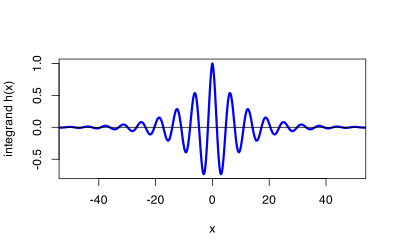
\includegraphics[keepaspectratio]{index_files/mediabag/lectures/L02-mc-uses_files/figure-pdf/h-graph-1.pdf}}

This suggests to me that a mean of 0 and a standard deviation of 20
might work quite well, since this will tend to take values in
\([-40,40]\) or so.

We will use R's function \texttt{dnorm()} for the probability density
function of the normal distribution (which saves us from having to
remember what that is).

\begin{Shaded}
\begin{Highlighting}[]
\NormalTok{n }\OtherTok{\textless{}{-}} \FloatTok{1e6}
\NormalTok{integrand }\OtherTok{\textless{}{-}} \ControlFlowTok{function}\NormalTok{(x) }\FunctionTok{exp}\NormalTok{(}\SpecialCharTok{{-}}\FloatTok{0.1} \SpecialCharTok{*} \FunctionTok{abs}\NormalTok{(x)) }\SpecialCharTok{*} \FunctionTok{cos}\NormalTok{(x)}
\NormalTok{pdf       }\OtherTok{\textless{}{-}} \ControlFlowTok{function}\NormalTok{(x) }\FunctionTok{dnorm}\NormalTok{(x, }\DecValTok{0}\NormalTok{, }\DecValTok{20}\NormalTok{)}
\NormalTok{phi       }\OtherTok{\textless{}{-}} \ControlFlowTok{function}\NormalTok{(x) }\FunctionTok{integrand}\NormalTok{(x) }\SpecialCharTok{/} \FunctionTok{pdf}\NormalTok{(x)}

\NormalTok{samples }\OtherTok{\textless{}{-}} \FunctionTok{rnorm}\NormalTok{(n, }\DecValTok{0}\NormalTok{, }\DecValTok{20}\NormalTok{)}
\FunctionTok{mean}\NormalTok{(}\FunctionTok{phi}\NormalTok{(samples))}
\end{Highlighting}
\end{Shaded}

\begin{verbatim}
[1] 0.2189452
\end{verbatim}

\end{example}

\textbf{Next time:} \emph{We will analyse the accuracy of these Monte
Carlo estimates.}

\textbf{Summary:}

\begin{itemize}
\item
  The indicator \(\Ind_A(x)\) function of a set \(A\) is 1 if
  \(x \in A\) or 0 if \(x \notin A\).
\item
  We can estimate a probability \(\mathbb P(X \in A)\) by using the
  Monte Carlo estimate for \(\Exg\Ind_A(X)\).
\item
  We can estimate an integral \(\int h(x) \, \mathrm{d}x\) by using a
  Monte Carlo estimate with \(\phi(x)\,f(x) = h(x)\).
\end{itemize}

\textbf{Read more:}
\href{https://leeds.primo.exlibrisgroup.com/permalink/44LEE_INST/1fj430b/cdi_askewsholts_vlebooks_9781118728031}{Voss,
\emph{An Introduction to Statistical Computing}}, Section 3.1 and
Subsection 3.2.1.

\chapter{Monte Carlo error I: theory}\label{monte-carlo-error-i-theory}

\[ \]

\section{Estimation error}\label{estimation-error}

Today we are going to analysing the accuracy of Monte Carlo estimation.
But before talking about Monte Carlo estimation specifically, let's
first remind ourselves of some concepts about error in statistical
estimation more generally. We will use the following definitions.

\begin{definition}[]\protect\hypertarget{def-stats}{}\label{def-stats}

Let \(\widehat\theta\) be an estimator of a parameter \(\theta\). Then
we have the following definitions of the estimator \(\widehat\theta\):

\begin{itemize}
\item
  The \textbf{bias} is
  \(\operatorname{bias}\big(\widehat\theta\big) = \mathbb E\big(\widehat\theta - \theta\big)  = \mathbb E\widehat\theta - \theta\).
\item
  The \textbf{mean-square error} is
  \(\operatorname{MSE}\big(\widehat\theta\big) = \mathbb E \big(\widehat\theta - \theta\big)^2\).
\item
  The \textbf{root-mean-square error} is the square-root of the
  mean-square error,
  \[\operatorname{RMSE}\big(\widehat\theta\big) = \sqrt{\operatorname{MSE}(\widehat\theta)} = \sqrt{\mathbb E (\widehat\theta - \theta)^2} . \]
\end{itemize}

\end{definition}

Usually, the main goal of estimation is to get the mean-square error of
an estimate as small as possible. This is because the MSE measures by
what distance we are missing on average. It can be easier to interpret
what the root-mean-square error means, as the RMSE has the same units as
the parameter being measured: if \(\theta\) and \(\widehat{\theta}\) are
in metres, say, then the MSE is in metres-squared, whereas the RMSE
error is in metres again. If you minimise the MSE you also minimise the
RMSE and vice versa.

It's nice to have an ``unbiased'' estimator -- that is, one with bias 0.
This is because bias measures any systematic error in a particular
direction. However, unbiasedness by itself is not enough for an estimate
to be good -- we need low variance too. (Remember the old joke about the
statistician who misses his first shot ten yards to the left, misses his
second shot ten yards to the right, then claims to have ``hit the target
on average.'')

(Remember also that ``bias'' is simply the word statisticians use for
\(\mathbb E(\widehat\theta - \theta)\); we don't mean ``bias'' in the
derogatory way it is sometimes used in political arguments, for
example.)

You probably also remember the relationship between the mean-square
error, the bias, and the variance:

\begin{theorem}[]\protect\hypertarget{thm-MSE-bias}{}\label{thm-MSE-bias}

~
\(\operatorname{MSE}\big(\widehat\theta\big) = \operatorname{bias}\big(\widehat\theta\big)^2 + \operatorname{Var}\big(\widehat\theta\big)\).

\end{theorem}

\begin{proof}
The MSE is \begin{align}
  \operatorname{MSE}\big(\widehat\theta\big) = \Exg\big(\widehat\theta - \theta\big)^2
    &= \Exg \big(\widehat\theta^2 - 2\theta\widehat\theta + \theta\big)^2 \\
    &= \Exg \widehat\theta^2 - 2\theta \Exg \widehat\theta + \theta^2 ,
\end{align} where we have expanded the brackets and bought the
expectation inside (remembering that \(\theta\) is a constant). Since
the variance can be written as
\(\Var(\widehat\theta) = \Exg\widehat\theta^2 - (\Exg \widehat\theta)^2\),
we can use a cunning trick of both subtracting and adding
\((\Exg \widehat\theta)^2\). This gives \begin{align}
\operatorname{MSE}\big(\widehat\theta\big)
  &= \Exg \widehat\theta^2 - \big(\!\Exg \widehat\theta\big)^2 + \big(\!\Exg \widehat\theta\big)^2 - 2\theta \Exg \widehat\theta + \theta^2 \\
  &= \Var\big(\widehat\theta\big) + \big( (\Exg \widehat\theta)^2 - 2\theta \Exg \widehat\theta + \theta^2 \big) \\
  &= \Var\big(\widehat\theta\big) + \big( \! \Exg \widehat\theta - \theta\big)^2 \\
  &= \Var\big(\widehat\theta\big) + \operatorname{bias}(\widehat\theta)^2 .
\end{align} This proves the result.
\end{proof}

Since the bias contributes to the mean-square error, that's another
reason to like estimator with low -- or preferably zero -- bias. But
again, unbiasedness isn't enough by itself; we want low variance too.
(There are some situations where there's a ``bias--variance tradeoff'',
where allowing some bias reduces the variance and so can reduce the MSE.
It turns out that Monte Carlo is not one of these cases, however.)

\section{Error of Monte Carlo estimator:
theory}\label{error-of-monte-carlo-estimator-theory}

In this lecture, we're going to be looking more carefully at the size of
the errors made by the Monte Carlo estimator
\[ \widehat{\theta}_n^{\mathrm{MC}} = \frac{1}{n} \big(\phi(X_1) + \phi(X_2) + \cdots + \phi(X_n) \big) = \frac{1}{n} \sum_{i=1}^n \phi(X_i) . \]

Our main result is the following.

\begin{theorem}[]\protect\hypertarget{thm-MCerr}{}\label{thm-MCerr}

Let \(X\) be a random variable, \(\phi\) a function, and
\(\theta = \Exg\phi(X)\). Let
\[ \widehat{\theta}_n^{\mathrm{MC}} = \frac{1}{n} \sum_{i=1}^n \phi(X_i) \]
be the Monte Carlo estimator of \(\theta\). Then:

\begin{enumerate}
\def\labelenumi{\arabic{enumi}.}
\item
  \(\widehat{\theta}_n^{\mathrm{MC}}\) is unbiased, in that
  \(\operatorname{bias}\big(\widehat{\theta}_n^{\mathrm{MC}}\big) = 0\).
\item
  The variance of of \(\widehat{\theta}_n^{\mathrm{MC}}\) is
  \({\displaystyle \operatorname{Var}\big(\widehat{\theta}_n^{\mathrm{MC}}\big) = \frac{1}{n} \operatorname{Var}\big(\phi(X)\big)}\).
\item
  The mean-square error of \(\widehat{\theta}_n^{\mathrm{MC}}\) is
  \({\displaystyle \operatorname{MSE}\big(\widehat{\theta}_n^{\mathrm{MC}}\big) = \frac{1}{n} \operatorname{Var}\big(\phi(X)\big)}\).
\item
  The root-mean-square error of \(\widehat{\theta}_n^{\mathrm{MC}}\) is
  \[{\displaystyle \operatorname{RMSE}\big(\widehat{\theta}_n^{\mathrm{MC}}\big) = \sqrt{\frac{1}{n} \operatorname{Var}\big(\phi(X)\big)} = \frac{1}{\sqrt{n}} \, \operatorname{sd}\big(\phi(X)\big)}. \]
\end{enumerate}

\end{theorem}

Before we get to the proof, let's recap some relevant probability.

Let \(Y_1, Y_2, \dots\) be IID random variables with common expectation
\(\mathbb EY_1 = \mu\) and common variance
\(\operatorname{Var}(Y_1) = \sigma^2\). Consider the mean of the first
\(n\) random variables,
\[ \overline{Y}_n = \frac{1}{n} \sum_{i=1}^n Y_i . \] Then the
expectation of \(\overline{Y}_n\) is
\[ \mathbb E \overline{Y}_n = \mathbb E\left(\frac{1}{n}\sum_{i=1}^n Y_i\right) = \frac{1}{n} 
\sum_{i=1}^n \mathbb{E}Y_i = \frac{1}{n}\,n\,\mu = \mu . \] The variance
of \(\overline{Y}_n\) is
\[ \operatorname{Var}\big(  \overline{Y}_n \big)= \operatorname{Var} \left(\frac{1}{n}\sum_{i=1}^n Y_i\right) = \bigg(\frac{1}{n}\bigg)^2 
\sum_{i=1}^n \operatorname{Var}(Y_i) = \frac{1}{n^2}\,n\,\sigma^2 = \frac{\sigma^2}{n} , \]
where, for this one, we used the independence of the random variables.

\begin{proof}
Apply the probability facts from above with \(Y = \phi(X)\). This gives:

\begin{enumerate}
\def\labelenumi{\arabic{enumi}.}
\item
  \(\Ex \widehat{\theta}_n^{\mathrm{MC}} = \Ex \overline Y_n = \Ex Y = \Exg \phi(X)\),
  so
  \(\operatorname{bias}(\widehat{\theta}_n^{\mathrm{MC}}) = \Exg \phi(X) - \Exg \phi(X) = 0\).
\item
  \({\displaystyle \operatorname{Var}\big(\widehat{\theta}_n^{\mathrm{MC}}\big) = \operatorname{Var}\big(\overline Y_n\big) = \frac{1}{n} \operatorname{Var}(Y) = \frac{1}{n} \operatorname{Var}\big(\phi(X)\big)}\).
\item
  Using Theorem~\ref{thm-MSE-bias},
  \[\operatorname{MSE}(\widehat{\theta}_n^{\mathrm{MC}}) = \operatorname{bias}(\widehat{\theta}_n^{\mathrm{MC}})^2 + \operatorname{Var}(\widehat{\theta}_n^{\mathrm{MC}}) = 0^2 + \frac{1}{n} \operatorname{Var}\big(\phi(X)\big) = \frac{1}{n} \operatorname{Var}\big(\phi(X)\big) . \]
\item
  Take the square root of part 3.
\end{enumerate}

\end{proof}

Let's think about MSE \(\frac{1}{n} \Var(\phi(X))\). The variance terms
is some fixed fact about the random variable \(X\) and the function
\(\phi\). So as \(n\) gets bigger, \(\frac{1}{n}\) gets smaller, so the
MSE gets smaller, and the estimator gets more accurate. This goes back
to what we said when we introduced the Monte Carlo estimator: we get a
more accurate estimate by increasing \(n\). More specifically, the MSE
scales like \(1/n\), or -- perhaps a more useful result -- the RMSE
scales like \(1/\sqrt{n}\). We'll come back to this in the next lecture.

\section{Error of Monte Carlo estimator:
practice}\label{error-of-monte-carlo-estimator-practice}

So when we form a Monte Carlo estimate \(\hat\theta_n^{\text{MC}}\), we
now know it will be unbiased. We'd also like to know it's mean-square
and/or root-mean-square error too.

There's a problem here, though. The reason we are doing Monte Carlo
estimation in the first place is that we \emph{couldn't} calculate
\(\Exg \phi(X)\). So it seems very unlikely we'll be able to calculate
the variance \(\operatorname{Var}(\phi(X))\) either. So how will be able
to assess the mean-square (or root-mean-square) error of our Monte Carlo
estimator?

Well, we can't know it exactly. But we \emph{can} estimate the variance
from the samples we are already using: by taking the sample variance of
the samples \(\phi(x_i)\). That is, we can estimate the variance of the
Monte Carlo estimator by the sample variance
\[ S^2 = \frac{1}{n-1} \sum_{i=1}^n \big(\phi(X_i) - \widehat{\theta}_n^{\mathrm{MC}} \big)^2 . \]
Then we can similarly estimate the mean-square and root-mean-square
errors by
\[ \text{MSE} \approx \frac{1}{n}S^2 \qquad \text{and} \qquad \text{RMSE} \approx \sqrt{\frac{1}{n} S^2} = \frac{1}{\sqrt{n}}\,S  \]
respectively.

\begin{example}[]\protect\hypertarget{exm-MCexp2}{}\label{exm-MCexp2}

Let's go back to the very first example in the module,
Example~\ref{exm-MCexp}, where we were trying to find the expectation of
an \(\operatorname{Exp}(2)\) random variable. We used this R code:

\begin{Shaded}
\begin{Highlighting}[]
\NormalTok{n }\OtherTok{\textless{}{-}} \FloatTok{1e6}
\NormalTok{samples }\OtherTok{\textless{}{-}} \FunctionTok{rexp}\NormalTok{(n, }\DecValTok{2}\NormalTok{)}
\NormalTok{MCest }\OtherTok{\textless{}{-}} \FunctionTok{mean}\NormalTok{(samples)}
\NormalTok{MCest}
\end{Highlighting}
\end{Shaded}

\begin{verbatim}
[1] 0.5006352
\end{verbatim}

(Because Monte Carlo estimation is random, this won't be the
\emph{exact} same estimate we had before, of course.)

So if we want to investigate the error, we can use the sample variance
of these samples. We will use the sample variance function
\texttt{var()} to calculate the sample variance. In this simple case,
the function is \(\phi(x) = x\), so we need only use the variance of the
samples themselves.

\begin{Shaded}
\begin{Highlighting}[]
\NormalTok{var\_est }\OtherTok{\textless{}{-}} \FunctionTok{var}\NormalTok{(samples)}
\NormalTok{MSEest  }\OtherTok{\textless{}{-}}\NormalTok{ var\_est }\SpecialCharTok{/}\NormalTok{ n}
\NormalTok{RMSEest }\OtherTok{\textless{}{-}} \FunctionTok{sqrt}\NormalTok{(MSEest)}
\FunctionTok{c}\NormalTok{(var\_est, MSEest, RMSEest)}
\end{Highlighting}
\end{Shaded}

\begin{verbatim}
[1] 2.503570e-01 2.503570e-07 5.003569e-04
\end{verbatim}

The first number is \texttt{var\_est} \(= 0.2504\), the sample variance
of our \(\phi(x_i)\)s:\\
\[ s^2 = \frac{1}{n-1} \sum_{i=1}^n \big(\phi(x_i) - \widehat{\theta}_n^{\mathrm{MC}}\big)^2 . \]
This should be a good estimate of the true variance
\(\operatorname{Var}(\phi(X))\). (In fact, in this simple case, we know
that \(\operatorname{Var}(X) = \frac{1}{2^2} = 0.25\), so we know that
the estimate is good.) In calculating this in the code, we used R's
\texttt{var()} function, which calculates the sample variance of some
values.

The second number is \texttt{MSEest}
\(= \ensuremath{2.504\times 10^{-7}}\), our estimate of the mean-square
error. Since
\(\operatorname{MSE}(\widehat{\theta}_n^{\mathrm{MC}}) = \frac{1}{n} \operatorname{Var}(\phi(X))\),
then \(\frac{1}{n} S^2\) should be a good estimate of the MSE.

The third number is \texttt{RMSEest} \(= \ensuremath{5\times 10^{-4}}\)
our estimate of the root-mean square error, which is simply the
square-root of our estimate of the mean-square error.

\end{example}

\begin{example}[]\protect\hypertarget{exm-MCprob2}{}\label{exm-MCprob2}

In Example~\ref{exm-MCprob}, we were estimating \(\mathbb P(Z > 2)\),
where \(Z\) is a standard normal.

Our code was

\begin{Shaded}
\begin{Highlighting}[]
\NormalTok{n }\OtherTok{\textless{}{-}} \FloatTok{1e6}
\NormalTok{samples }\OtherTok{\textless{}{-}} \FunctionTok{rnorm}\NormalTok{(n)}
\NormalTok{MCest }\OtherTok{\textless{}{-}} \FunctionTok{mean}\NormalTok{(samples }\SpecialCharTok{\textgreater{}} \DecValTok{2}\NormalTok{)}
\NormalTok{MCest}
\end{Highlighting}
\end{Shaded}

\begin{verbatim}
[1] 0.022458
\end{verbatim}

So our root-mean-square error can be approximated as

\begin{Shaded}
\begin{Highlighting}[]
\NormalTok{MSEest }\OtherTok{\textless{}{-}} \FunctionTok{var}\NormalTok{(samples }\SpecialCharTok{\textgreater{}} \DecValTok{2}\NormalTok{) }\SpecialCharTok{/}\NormalTok{ n}
\FunctionTok{sqrt}\NormalTok{(MSEest)}
\end{Highlighting}
\end{Shaded}

\begin{verbatim}
[1] 0.0001481677
\end{verbatim}

since \texttt{samples\ \textgreater{}\ 2} is the indicator function of
whether \(X_i > 2\) or not.

\end{example}

\textbf{Next time:} \emph{We'll continue analysing Monte Carlo error,
looking at confidence intervals and assessing how many samples to
take..}

\textbf{Summary:}

\begin{itemize}
\item
  The Monte Carlo estimator is unbiased.
\item
  The Monte Carlo estimator has mean-square error \(\Var(\phi(X))/n\),
  so the root-mean-square error scales like \(1/\sqrt{n}\).
\item
  The mean-square error can be estimated by \(S^2 / n\), where \(S^2\)
  is the sample variance of the \(\phi(X_i)\).
\end{itemize}

\textbf{Read more:}
\href{https://leeds.primo.exlibrisgroup.com/permalink/44LEE_INST/1fj430b/cdi_askewsholts_vlebooks_9781118728031}{Voss,
\emph{An Introduction to Statistical Computing}}, Subsection 3.2.2.

\chapter{Monte Carlo error II:
practice}\label{monte-carlo-error-ii-practice}

\[ \]

\section{Recap}\label{recap}

Let's recap where we've got to. We know that the Monte Carlo estimator
for \(\theta = \Exg \phi(X)\) is
\[ \widehat{\theta}_n^{\mathrm{MC}} = \frac{1}{n} \sum_{i=1}^n \phi(X_i) .\]
Last time, we saw that the Monte Carlo estimator is unbiased, and that
its mean-square and root-mean-square errors are
\[ \operatorname{MSE}\big(\widehat{\theta}_n^{\mathrm{MC}}\big) = \frac{1}{n} \operatorname{Var}\big(\phi(X)\big) \qquad \operatorname{RMSE}\big(\widehat{\theta}_n^{\mathrm{MC}}\big) = \sqrt{\frac{1}{n} \operatorname{Var}\big(\phi(X)\big)} . \]
We saw that these themselves can be estimated as \(S^2/n\) and
\(S/\sqrt{n}\) respectively, where \(S^2\) is the sample variance of the
\(\phi(X_i)\)s.

\section{Confidence intervals}\label{confidence-intervals}

So far, we have described our error tolerance in terms of the MSE or
RMSE. But we could have talked about ``confidence intervals'' or
``margins of error'' instead. This might be easier to understand for
non-mathematicians, for whom ``root-mean-square error'' doesn't really
mean anything.

Here, we will want to appeal to the central limit theorem approximation.
A bit more probability revision: Let \(Y_1, Y_2, \dots\) be IID again,
with expectation \(\mu\) and variance \(\sigma^2\). Write
\(\overline Y_n\) for the mean. We've already reminded ourselves of the
law of large numbers, which says that \(\overline Y_n \to \mu\) as
\(n \to infty\). Then in the last lecture we saw that
\(\mathbb E \overline Y_n = \mu\) and
\(\Var(\overline{Y}_n) = \sigma^2/n\). The \textbf{central limit
theorem} says that the distribution of \(\overline Y_n\) is
approximately normally distributed with those parameters, so
\(\overline Y_n \approx \operatorname{N}(\mu, \sigma^2/n)\) when \(n\)
is large. (This is an informal statement of the central limit theorem:
you probably know some more formal ways to more precisely state it, but
this will do for us.)

Recall that, in the normal distribution
\(\operatorname{N}(\mu, \sigma^2)\), we expect to be within \(1.96\)
standard deviations of the mean with 95\% probability. More generally,
the interval
\([\mu - q_{1-\alpha/2}\sigma, \mu + q_{1-\alpha/2}\sigma]\), where
\(q_{1-\alpha/2}\) is the \((1- \frac{\alpha}{2})\)-quantile of the
normal distribution, contains the true value with probability
approximately \(1 - \alpha\).

We can form an approximate confidence interval for a Monte Carlo
estimate using this idea. We have our Monte Carlo estimator
\(\widehat{\theta}_n^\mathrm{MC}\) as our estimator of the \(\mu\)
parameter, and our estimator of the root-mean-square error
\(S/\sqrt{n}\) as our estimator of the \(\sigma\) parameter. So our
confidence interval is estimated as
\[\bigg[ \widehat{\theta}_n^\mathrm{MC} - q_{1-\alpha/2}\,\frac{S}{\sqrt{n}}, \ \widehat{\theta}_n^\mathrm{MC} + q_{1-\alpha/2}\,\frac{S}{\sqrt{n}} \bigg] . \]

\begin{example}[]\protect\hypertarget{exm-MCprob3}{}\label{exm-MCprob3}

We continue the example of Example~\ref{exm-MCprob} and
Example~\ref{exm-MCprob2}, where we were estimating \(\mathbb P(Z > 2)\)
for \(Z\) a standard normal.

\begin{Shaded}
\begin{Highlighting}[]
\NormalTok{n }\OtherTok{\textless{}{-}} \FloatTok{1e6}
\NormalTok{samples }\OtherTok{\textless{}{-}} \FunctionTok{rnorm}\NormalTok{(n)}
\NormalTok{MCest   }\OtherTok{\textless{}{-}} \FunctionTok{mean}\NormalTok{(samples }\SpecialCharTok{\textgreater{}} \DecValTok{2}\NormalTok{)}
\NormalTok{RMSEest }\OtherTok{\textless{}{-}} \FunctionTok{sqrt}\NormalTok{(}\FunctionTok{var}\NormalTok{(samples }\SpecialCharTok{\textgreater{}} \DecValTok{2}\NormalTok{) }\SpecialCharTok{/}\NormalTok{ n)}
\NormalTok{MCest}
\end{Highlighting}
\end{Shaded}

\begin{verbatim}
[1] 0.023177
\end{verbatim}

Our confidence interval is estimates as follows

\begin{Shaded}
\begin{Highlighting}[]
\NormalTok{alpha }\OtherTok{\textless{}{-}} \FloatTok{0.05}
\NormalTok{quant }\OtherTok{\textless{}{-}} \FunctionTok{qnorm}\NormalTok{(}\DecValTok{1} \SpecialCharTok{{-}}\NormalTok{ alpha }\SpecialCharTok{/} \DecValTok{2}\NormalTok{)}
\FunctionTok{c}\NormalTok{(MCest }\SpecialCharTok{{-}}\NormalTok{ quant }\SpecialCharTok{*}\NormalTok{ RMSEest, MCest }\SpecialCharTok{+}\NormalTok{ quant }\SpecialCharTok{*}\NormalTok{ RMSEest)}
\end{Highlighting}
\end{Shaded}

\begin{verbatim}
[1] 0.02288209 0.02347191
\end{verbatim}

\end{example}

\section{How many samples do I need?}\label{how-many-samples-do-i-need}

In our examples we've picked the number of samples \(n\) for our
estimator, then approximated the error based on that. But we could do
things the other way around -- fix an error tolerance that we're willing
to deal with, then work out what sample size we need to achieve it.

We know that the root-mean-square error is
\[ \operatorname{RMSE}\big(\widehat{\theta}_n^{\mathrm{MC}}\big) = \sqrt{\frac{1}{n} \operatorname{Var}\big(\phi(X)\big)} \]
So if we want to get the RMSE down to \(\epsilon\), say, then this shows
that we need
\[ \epsilon = \sqrt{\frac{1}{n} \operatorname{Var}\big(\phi(X)\big)} .\]
Squaring both sides, multiplying both sides by \(n\), and dividing both
sides by \(\epsilon^2\) gives
\[ n = \frac{1}{\epsilon^2} \Var\big(\phi(X)\big) . \]

So this tells us how many samples \(n\) we need. Except we still have a
problem here, though. We (usually) don't know \(\Var(\phi(X))\). But we
can't even \emph{estimate} \(\Var(\phi(X))\) until we've already taken
the samples. So it seems we're stuck.

But we can use this idea with a three-step process:

\begin{enumerate}
\def\labelenumi{\arabic{enumi}.}
\item
  Run an initial ``pilot'' Monte Carlo algorithm with a small number of
  samples \(n\). Use the results of the ``pilot'' to estimate the
  variance \(S^2 \approx \Var(\phi(X))\). We want \(n\) small enough
  that this runs very quickly, but big enough that we get a reasonably
  OK estimate of the variance.
\item
  Pick a desired RMSE accuracy \(\epsilon\). We now know that we require
  roughly \(N = S^2 / \epsilon^2\) samples to get our desired accuracy.
\item
  Run the ``real'' Monte Carlo algorithm with this big number of samples
  \(N\). We will put up with this being quite slow, because we know
  we're definitely going to get the error tolerance we need.
\end{enumerate}

(We could potentially use further steps, where we now check the variance
with the ``real'' big-\(N\) samples, and, if we learn we had
underestimated in Step 1, take even more samples to correct for this.)

\begin{example}[]\protect\hypertarget{exm-MC22}{}\label{exm-MC22}

Let's try this with Example~\ref{exm-MC2} from before. We were trying to
estimate \(\mathbb{E}(\sin X)\), where
\(X \sim \operatorname{N}(1, 2^2)\).

We'll start with just \(n = 1000\) samples, for our pilot study.

\begin{Shaded}
\begin{Highlighting}[]
\NormalTok{n\_pilot }\OtherTok{\textless{}{-}} \DecValTok{1000}
\NormalTok{samples }\OtherTok{\textless{}{-}} \FunctionTok{rnorm}\NormalTok{(n\_pilot, }\DecValTok{1}\NormalTok{, }\DecValTok{2}\NormalTok{)}
\NormalTok{var\_est }\OtherTok{\textless{}{-}} \FunctionTok{var}\NormalTok{(}\FunctionTok{sin}\NormalTok{(samples))}
\NormalTok{var\_est}
\end{Highlighting}
\end{Shaded}

\begin{verbatim}
[1] 0.4905153
\end{verbatim}

This was very quick! We won't have got a super-accurate estimate of
\(\mathbb E\phi(X)\), but we have a reasonable idea of roughly what
\(\operatorname{Var}(\phi(X))\) is. This will allow us to pick out
``real'' sample size in order to get a root-mean-square error of
\(10^{-4}\).

\begin{Shaded}
\begin{Highlighting}[]
\NormalTok{epsilon }\OtherTok{\textless{}{-}} \FloatTok{1e{-}4}
\NormalTok{n\_real  }\OtherTok{\textless{}{-}} \FunctionTok{round}\NormalTok{(var\_est }\SpecialCharTok{/}\NormalTok{ epsilon}\SpecialCharTok{\^{}}\DecValTok{2}\NormalTok{)}
\NormalTok{n\_real}
\end{Highlighting}
\end{Shaded}

\begin{verbatim}
[1] 49051535
\end{verbatim}

This tells us that we will need about 50 million samples! This is a lot,
but now we know we're going to get the accuracy we want, so it's worth
it. (In this particular case, 50 million samples will only take a few
second on a modern computer. But generally, once we know our code works
and we know how many samples we will need for the desired accuracy, this
is the sort of thing that we could leave running overnight or whatever.)

\begin{Shaded}
\begin{Highlighting}[]
\NormalTok{samples }\OtherTok{\textless{}{-}} \FunctionTok{rnorm}\NormalTok{(n\_real, }\DecValTok{1}\NormalTok{, }\DecValTok{2}\NormalTok{)}
\NormalTok{MCest }\OtherTok{\textless{}{-}} \FunctionTok{mean}\NormalTok{(}\FunctionTok{sin}\NormalTok{(samples))}
\NormalTok{MCest}
\end{Highlighting}
\end{Shaded}

\begin{verbatim}
[1] 0.1139149
\end{verbatim}

\begin{Shaded}
\begin{Highlighting}[]
\NormalTok{RMSEest }\OtherTok{\textless{}{-}} \FunctionTok{sqrt}\NormalTok{(}\FunctionTok{var}\NormalTok{(}\FunctionTok{sin}\NormalTok{(samples)) }\SpecialCharTok{/}\NormalTok{ n\_real)}
\NormalTok{RMSEest}
\end{Highlighting}
\end{Shaded}

\begin{verbatim}
[1] 9.964886e-05
\end{verbatim}

This second step was quite slow (depending on the speed of the computer
being used -- it was only about 5 seconds on my pretty-new laptop, but
slower on my ancient work desktop). But we see that we have indeed got
our Monte Carlo estimate to (near enough) the desired accuracy.

\end{example}

Generally, if we want a more accurate Monte Carlo estimator, we can just
take more samples. But the equation
\[ n = \frac{1}{\epsilon^2} \Var\big(\phi(X)\big) \] is actually quite
bad news. To get an RMSE of \(\epsilon\) we need order \(1/\epsilon^2\)
samples. That's not good. Think of it like this: to \emph{double} the
accuracy we need to \emph{quadruple} the number of samples. Even worse:
to get ``one more decimal place of accuracy'' means dividing
\(\epsilon\) by ten; but that means multiplying the number of samples by
one hundred!

More samples take more time, and cost more energy and money. Wouldn't it
be nice to have some better ways of increasing the accuracy of a Monte
Carlo estimate besides just taking more and more samples?

\textbf{Next time:} \emph{We begin our study of clever ``variance
reduction'' methods for Monte Carlo estimation.}

\textbf{Summary:}

\begin{itemize}
\item
  We can approximate confidence intervals for a Monte Carlo estimate by
  using a normal approximation.
\item
  To get the root-mean-square error below \(\epsilon\) we need
  \(n = \Var(\phi(X))/\epsilon^2\) samples.
\item
  We can use a two-step process, where a small ``pilot'' Monte Carlo
  estimation allows us to work out how many samples we will need for the
  big ``real'' estimation.
\end{itemize}

\textbf{Read more:}
\href{https://leeds.primo.exlibrisgroup.com/permalink/44LEE_INST/1fj430b/cdi_askewsholts_vlebooks_9781118728031}{Voss,
\emph{An Introduction to Statistical Computing}}, Subsections
3.2.2--3.2.4.

\chapter{Control variate}\label{control-variate}

\[ \]

\section{Variance reduction}\label{variance-reduction}

Let's recap where we've got to. The Monte Carlo estimator of
\(\theta = \Exg \phi(X)\) is
\[ \widehat{\theta}_n^{\mathrm{MC}} = \frac{1}{n} \sum_{i=1}^n \phi(X_i), \]
where \(X_1, X_2, \dots, X_n\) are IID random samples from \(X\). The
mean-square error of this estimator is
\[{\displaystyle \operatorname{MSE}\big(\widehat{\theta}_n^{\mathrm{MC}}\big) = \frac{1}{n} \operatorname{Var}\big(\phi(X)\big)} . \]
If we want a more accurate estimate, we can just take more samples
\(n\). But the problem is that the root-mean-square error scales like
\(1/\sqrt{n}\). To double the accuracy, we need four times as many
samples; for one more decimal place of accuracy, we need one hundred
times as many samples.

Are there other ways we could reduce the error of Monte Carlo
estimation, so we need fewer samples? That is, can we use some
mathematical ingenuity to adapt the Monte Carlo estimate to one with a
smaller error?

Well, the mean-square error is the variance divided by \(n\). So if we
can't (or don't want to) increase \(n\), perhaps we can \emph{decrease}
the \emph{variance} instead? Strategies to do this are called
\textbf{variance reduction strategies}. In this module, we will look at
three variance reduction strategies:

\begin{itemize}
\item
  \textbf{Control variate:} We can ``anchor'' our estimate of
  \(\Exg \phi(X)\) to a similar but easier-to-calculate value
  \(\Exg \psi(X)\). (This lecture)
\item
  \textbf{Antithetic variables:} Instead of using independent samples,
  we could use correlated samples. If the correlation is negative this
  can improve our estimate. (Lectures 6 and 7)
\item
  \textbf{Importance sampling:} Instead of sampling from \(X\), sample
  from some other more suitable distribution instead, then adjust the
  answer we get. (Lectures 8 and 9)
\end{itemize}

\section{Control variate estimation}\label{control-variate-estimation}

In Monday's lecture, I polled the class on this question: \emph{Estimate
the average time it takes to fly from London to New York.}

\begin{itemize}
\item
  The actual answer is: 8 hours.
\item
  The mean guess was: 9 hours and 38 minutes (98 minutes too much)
\item
  The root-mean-square error for the guesses was: 158 minutes
\end{itemize}

After you'd guessed, I gave the following hint: \emph{Hint: The average
time it takes to fly from London to Washington D.C. is 8 hours and 15
minutes.} After the hint:

\begin{itemize}
\item
  The mean guess was: 8 hours and 50 minutes (50 minutes too much)
\item
  The root-mean-square error for the guesses was: 72 minutes
\end{itemize}

So after the hint, the error of the class was reduced by 55\%.

(Incidentally, you were about 30\% at guessing this than last year's
students\ldots)

Why did the hint help? We were trying to estimate
\(\theta^{\mathrm{NY}}\), the distance to New York. But that's a big
number, and the first estimates had a big error (over an hour, on
average). After the hint, I expect most people thought something like
this: ``The answer \(\theta^{\mathrm{NY}}\) is going to be similar to
the \(\theta^{\mathrm{DC}} =\) 8:15 to Washington D.C., but New York
isn't quite as far, so I should decrease the number a bit, but not too
much.''

To be more mathematical, we could write
\[\theta^{\mathrm{NY}} = \theta^{\mathrm{NY}} + \big(\theta^{\mathrm{DC}} - \theta^{\mathrm{DC}}\big) =  \underbrace{\theta^{\mathrm{DC}}\vphantom{\big)}}_{\text{known}} + \underbrace{\big(\theta^{\mathrm{NY}} - \theta^{\mathrm{DC}}\big)}_{\text{small}} . \]
In that equation, the first term, \(\theta^{\mathrm{DC}} =\) 8:15 was
completely known, so had error 0, while the second term
\(\theta^{\mathrm{NY}} - \theta^{\mathrm{DC}}\) (actually minus 15
minutes) was a small number, so only had a small error.

This idea of improving an estimate by ``anchoring'' it to some known
value is called \textbf{controlled estimation}. It is a very useful idea
in statistics (and in life!).

We can apply this idea to Monte Carlo estimation too. Suppose we are
trying to estimate \(\theta = \Exg \phi(X)\). We could look for a
function \(\psi\) that is similar to \(\phi\) (at least for the values
of \(x\) that have high probability for the random variable \(X\)), but
where we know for certain what \(\Exg \psi(X)\) is. Then we can write
\[ \theta = \Exg \phi(X) = \Exg \big(\phi(X) - \psi(X) + \psi(X)\big) = \underbrace{\Exg\big(\phi(X) - \psi(X)\big)}_{\text{estimate this with Monte Carlo}} + \underbrace{\Exg \psi(X)\vphantom{\big)}}_{\text{known}} . \]

Here, \(\psi(X)\) is known as the \textbf{control variate}.

\begin{definition}[]\protect\hypertarget{def-MCest}{}\label{def-MCest}

Let \(X\) be a random variable, \(\phi\) a function, and write
\(\theta = \Exg\phi(X)\). Let \(\psi\) be a function such that
\(\eta = \Exg\psi(X)\) is known. Suppose that \(X_1, X_2, \dots, X_n\)
are a random sample from \(X\). Then the \textbf{control variate Monte
Carlo estimate} \(\widehat\theta_n^{\mathrm{CV}}\) of \(\theta\) is
\[ \widehat{\theta}_n^{\mathrm{CV}} = \frac{1}{n} \sum_{i=1}^n \big(\phi(X_i) - \psi(X_i)\big) + \eta . \]

\end{definition}

\begin{example}[]\protect\hypertarget{exm-control}{}\label{exm-control}

Let's try to estimate \(\Ex \cos(X)\), where
\(X \sim \operatorname{N}(0,1)\) is a standard normal distribution.

We could do this the ``usual'' Monte Carlo way.

\begin{Shaded}
\begin{Highlighting}[]
\NormalTok{n }\OtherTok{\textless{}{-}} \FloatTok{1e6}
\NormalTok{phi }\OtherTok{\textless{}{-}} \ControlFlowTok{function}\NormalTok{(x) }\FunctionTok{cos}\NormalTok{(x)}
\NormalTok{samples }\OtherTok{\textless{}{-}} \FunctionTok{rnorm}\NormalTok{(n)}
\NormalTok{MCest }\OtherTok{\textless{}{-}} \FunctionTok{mean}\NormalTok{(}\FunctionTok{phi}\NormalTok{(samples))}
\NormalTok{MCest}
\end{Highlighting}
\end{Shaded}

\begin{verbatim}
[1] 0.6067224
\end{verbatim}

But we could see if we can do better with a control variate. But what
should we pick for the control function \(\psi\)? We want something
that's similar to \(\phi(x) = \cos(x)\), but where we can actually
calculate the expectation.

Here's a suggestion. If we remember our
\href{https://en.wikipedia.org/wiki/Taylor_series}{Taylor series}, we
know that, for \(x\) near \(0\),
\[ \cos x \approx 1 - \frac{x^2}{2!} + \frac{x^4}{4!} - \frac{x^6}{6!} + \cdots . \]
So how about taking the first two nonzero terms in the Taylor series
\[ \psi(x) = 1 - \frac{x^2}{2} . \] That is quite close to \(\cos x\),
at least for the values of \(x\) near 0 that
\(X \sim \operatorname{N}(0,1)\) is most likely to take.

\begin{Shaded}
\begin{Highlighting}[]
\FunctionTok{curve}\NormalTok{(}
  \FunctionTok{cos}\NormalTok{(x), }\AttributeTok{from =} \SpecialCharTok{{-}}\FloatTok{4.5}\NormalTok{, }\AttributeTok{to =} \FloatTok{4.5}\NormalTok{,}
  \AttributeTok{col =} \StringTok{"blue"}\NormalTok{, }\AttributeTok{lwd =} \DecValTok{3}\NormalTok{,}
  \AttributeTok{xlab =} \StringTok{"x"}\NormalTok{, }\AttributeTok{ylab =} \StringTok{""}\NormalTok{, }\AttributeTok{xlim =} \FunctionTok{c}\NormalTok{(}\SpecialCharTok{{-}}\DecValTok{4}\NormalTok{,}\DecValTok{4}\NormalTok{), }\AttributeTok{ylim =} \FunctionTok{c}\NormalTok{(}\SpecialCharTok{{-}}\FloatTok{1.2}\NormalTok{,}\FloatTok{1.2}\NormalTok{)}
\NormalTok{)}
\FunctionTok{curve}\NormalTok{(}\DecValTok{1} \SpecialCharTok{{-}}\NormalTok{ x}\SpecialCharTok{\^{}}\DecValTok{2} \SpecialCharTok{/} \DecValTok{2}\NormalTok{, }\AttributeTok{add =} \ConstantTok{TRUE}\NormalTok{, }\AttributeTok{col =} \StringTok{"red"}\NormalTok{, }\AttributeTok{lwd =} \DecValTok{2}\NormalTok{)}
\FunctionTok{legend}\NormalTok{(}
  \StringTok{"topright"}\NormalTok{, }\FunctionTok{c}\NormalTok{(}\StringTok{"cos x"}\NormalTok{, }\FunctionTok{expression}\NormalTok{(}\DecValTok{1} \SpecialCharTok{{-}}\NormalTok{ x}\SpecialCharTok{\^{}}\DecValTok{2} \SpecialCharTok{/} \DecValTok{2}\NormalTok{)),}
  \AttributeTok{lwd =} \FunctionTok{c}\NormalTok{(}\DecValTok{3}\NormalTok{, }\DecValTok{2}\NormalTok{), }\AttributeTok{col =} \FunctionTok{c}\NormalTok{(}\StringTok{"blue"}\NormalTok{, }\StringTok{"red"}\NormalTok{)}
\NormalTok{)}
\end{Highlighting}
\end{Shaded}

\pandocbounded{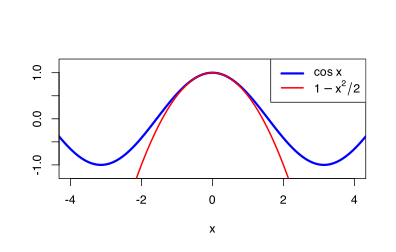
\includegraphics[keepaspectratio]{index_files/mediabag/lectures/L05-cv_files/figure-pdf/taylor-1.pdf}}

Not only that, but we know that for
\(Y \sim \operatorname{N}(\mu, \sigma^2)\) we have
\(\Ex Y^2 = \mu^2 + \sigma^2\). So
\[ \Exg \psi(X) = \Exg \left(1 - \frac{X^2}{2} \right) = 1 - \frac{\Ex X^2}{2} = 1 - \frac{0^2 + 1}{2} = \frac12 . \]

So our control variate estimate is:

\begin{Shaded}
\begin{Highlighting}[]
\NormalTok{psi }\OtherTok{\textless{}{-}} \ControlFlowTok{function}\NormalTok{(x) }\DecValTok{1} \SpecialCharTok{{-}}\NormalTok{ x}\SpecialCharTok{\^{}}\DecValTok{2} \SpecialCharTok{/} \DecValTok{2}
\NormalTok{CVest }\OtherTok{\textless{}{-}} \FunctionTok{mean}\NormalTok{(}\FunctionTok{phi}\NormalTok{(samples) }\SpecialCharTok{{-}} \FunctionTok{psi}\NormalTok{(samples)) }\SpecialCharTok{+} \DecValTok{1}\SpecialCharTok{/}\DecValTok{2}
\NormalTok{CVest}
\end{Highlighting}
\end{Shaded}

\begin{verbatim}
[1] 0.6060243
\end{verbatim}

\end{example}

\section{Error of control variate
estimate}\label{error-of-control-variate-estimate}

What is the error in a control variate estimate?

\begin{theorem}[]\protect\hypertarget{thm-CVerr}{}\label{thm-CVerr}

Let \(X\) be a random variable, \(\phi\) a function, and
\(\theta = \Exg\phi(X)\). Let \(\psi\) be a function such that
\(\eta \Exg\psi(X)\) is known. Let
\[ \widehat{\theta}_n^{\mathrm{CV}} = \frac{1}{n} \sum_{i=1}^n \big(\phi(X_i) - \psi(X_i)\big) + \eta\]
be the control variate Monte Carlo estimator of \(\theta\). Then:

\begin{enumerate}
\def\labelenumi{\arabic{enumi}.}
\item
  \(\widehat{\theta}_n^{\mathrm{CV}}\) is unbiased, in that
  \(\operatorname{bias}\big(\widehat{\theta}_n^{\mathrm{CV}}\big) = 0\).
\item
  The variance of of \(\widehat{\theta}_n^{\mathrm{CV}}\) is
  \({\displaystyle \operatorname{Var}\big(\widehat{\theta}_n^{\mathrm{CV}}\big) = \frac{1}{n} \operatorname{Var}\big(\phi(X) - \psi(X)\big)}\).
\item
  The mean-square error of \(\widehat{\theta}_n^{\mathrm{CV}}\) is
  \({\displaystyle \operatorname{MSE}\big(\widehat{\theta}_n^{\mathrm{CV}}\big) = \frac{1}{n} \operatorname{Var}\big(\phi(X) - \psi(X)\big)}\).
\item
  The root-mean-square error of \(\widehat{\theta}_n^{\mathrm{CV}}\) is
  \({\displaystyle \operatorname{RMSE}\big(\widehat{\theta}_n^{\mathrm{CV}}\big) = \frac{1}{\sqrt{n}} \sqrt{\operatorname{Var}\big(\phi(X) - \psi(X)\big)}}\).
\end{enumerate}

\end{theorem}

\begin{proof}
This is very similar to Theorem~\ref{thm-MCerr}, so we'll just sketch
the important differences.

In part 1, we have \begin{align*}
\Exg \widehat{\theta}_n^{\mathrm{CV}}
  &= \Exg \left(\frac{1}{n} \sum_{i=1}^n \big(\phi(X_i) - \psi(X_i)\big)\right) + \eta \\
  &= \frac{1}{n}\Exg \left(\sum_{i=1}^n \big(\phi(X_i) - \psi(X_i)\big)\right) + \eta \\
  &= \frac{n}{n}\Exg\big(\phi(X) - \psi(X)\big) + \eta \\
  &= \Exg\phi(X) - \Exg\psi(X) + \eta \\
  &= \Exg\phi(X) ,
\end{align*} since \(\eta = \Exg\psi(X)\). So the estimator is unbiased.

For part 2, remembering that \(\eta = \Exg \psi(X)\) is a constant, so
doesn't affect the variance, we have \begin{align*}
\Var \big(\widehat{\theta}_n^{\mathrm{CV}}\big)
&= \Var \left(\frac{1}{n} \sum_{i=1}^n \big(\phi(X_i) - \psi(X_i)\big) + \eta \right) \\
&= \Big( \frac{1}{n}\Big)^2 \Var \left(\sum_{i=1}^n \big(\phi(X_i) - \psi(X_i)\big) \right) \\
&= \frac{n}{n^2} \Var \big(\phi(X) - \psi(X)\big) \\
&= \frac{1}{n} \Var \big(\phi(X) - \psi(X)\big) .
\end{align*}

Parts 3 and 4 follow in the usual way.
\end{proof}

This tells us that a control variate Monte Carlo estimate is good when
the variance of \(\phi(X) - \psi(X)\). This variance is likely to be
small if \(\phi(X) - \psi(X)\) is usually small -- although, to be more
precise, it's more important for \(\phi(X) - \psi(X)\) to be
\emph{consistent}, rather than small per se.

As before, we can't usually calculate the variance
\(\Var(\phi(X) - \psi(X))\) exactly, but we can estimate it from the
samples. Again, we use the sample variance of \(\phi(X_i) - \psi(X_i)\),
\[S^2 = \frac{1}{n-1}\sum_{i=1}^n \Big(\big(\phi(X_i) - \psi(X_i)\big) - \big(\widehat\theta_n^{\mathrm{CV}} - \eta\big)\Big)^2 , \]
and estimate the MSE and RMSE by \(S^2 / n\) and \(S / \sqrt{n}\)
respectively.

\begin{example}[]\protect\hypertarget{exm-control2}{}\label{exm-control2}

We return to Example~\ref{exm-control}, where we were estimating
\(\Ex \cos(X)\) for \(X \sim \operatorname{N}(0,1)\).

The naive Monte Carlo estimate had mean-square and root-mean-square
error

\begin{Shaded}
\begin{Highlighting}[]
\NormalTok{n }\OtherTok{\textless{}{-}} \FloatTok{1e6}
\NormalTok{phi }\OtherTok{\textless{}{-}} \ControlFlowTok{function}\NormalTok{(x) }\FunctionTok{cos}\NormalTok{(x)}
\NormalTok{samples }\OtherTok{\textless{}{-}} \FunctionTok{rnorm}\NormalTok{(n)}
\NormalTok{MC\_MSE }\OtherTok{\textless{}{-}} \FunctionTok{var}\NormalTok{(}\FunctionTok{phi}\NormalTok{(samples)) }\SpecialCharTok{/}\NormalTok{ n}
\FunctionTok{c}\NormalTok{(MC\_MSE, }\FunctionTok{sqrt}\NormalTok{(MC\_MSE))}
\end{Highlighting}
\end{Shaded}

\begin{verbatim}
[1] 2.002522e-07 4.474955e-04
\end{verbatim}

The variance and root-mean-square error of our control variate estimate,
on the other hand, are

\begin{Shaded}
\begin{Highlighting}[]
\NormalTok{psi }\OtherTok{\textless{}{-}} \ControlFlowTok{function}\NormalTok{(x) }\DecValTok{1} \SpecialCharTok{{-}}\NormalTok{ x}\SpecialCharTok{\^{}}\DecValTok{2} \SpecialCharTok{/} \DecValTok{2}
\NormalTok{CV\_MSE }\OtherTok{\textless{}{-}} \FunctionTok{var}\NormalTok{(}\FunctionTok{phi}\NormalTok{(samples) }\SpecialCharTok{{-}} \FunctionTok{psi}\NormalTok{(samples)) }\SpecialCharTok{/}\NormalTok{ n}
\FunctionTok{c}\NormalTok{(CV\_MSE, }\FunctionTok{sqrt}\NormalTok{(CV\_MSE))}
\end{Highlighting}
\end{Shaded}

\begin{verbatim}
[1] 9.326675e-08 3.053960e-04
\end{verbatim}

This was a success! The mean-square error roughly halved, from
\(\ensuremath{2\times 10^{-7}}\) to \(\ensuremath{9.3\times 10^{-8}}\).
This meant the root-mean-square went down by about a third, from
\(\ensuremath{4.5\times 10^{-4}}\) to
\(\ensuremath{3.1\times 10^{-4}}\).

Halving the mean-square error would normally have required doubling the
number of samples \(n\), so we have effectively doubled the sample size
by using the control variate.

\end{example}

\textbf{Next time:} \emph{We look at our second variance reduction
technique: antithetic variables.}

\textbf{Summary:}

\begin{itemize}
\item
  Variance reduction techniques attempt to improve on Monte Carlo
  estimation making the variance smaller.
\item
  If we know \(\eta = \Exg \psi(X)\), then the control variate Monte
  Carlo estimate is
  \[ \widehat{\theta}_n^{\mathrm{CV}} = \frac{1}{n} \sum_{i=1}^n \big(\phi(X_i) - \psi(X_i)\big) + \eta.\]
\item
  The mean-square error of the control variate Monte Carlo estimate is
  \[{\displaystyle \operatorname{MSE}\big(\widehat{\theta}_n^{\mathrm{MC}}\big) = \frac{1}{n} \operatorname{Var}\big(\phi(X) - \psi(X)\big)}.\]
\end{itemize}

\textbf{Read more:}
\href{https://leeds.primo.exlibrisgroup.com/permalink/44LEE_INST/1fj430b/cdi_askewsholts_vlebooks_9781118728031}{Voss,
\emph{An Introduction to Statistical Computing}}, Subsection 3.3.3.

\chapter{Antithetic variables I}\label{antithetic-variables-i}

\[ \]

\section{Estimation with correlation}\label{estimation-with-correlation}

This lecture and the next, we will be looking at our second variance
reduction method for Monte Carlo estimation: the use of antithetic
variables.'' The word ``antithetic'' refers to using negative
correlation to reduce the variance an estimator.

Let's start with the simple example of estimating an expectation from
\(n = 2\) samples. Suppose \(Y\) has expectation \(\mu = \Ex Y\) and
variance \(\Var(Y) = \sigma^2\). Suppose \(Y_1\) and \(Y_2\) are
independent samples from \(Y\). Then the Monte Carlo estimator is
\[ \overline Y = \tfrac12(Y_1 + Y_2) . \] This estimator is unbiased,
since
\[ \Ex \overline Y = \Ex \big(\tfrac12(Y_1 + Y_2)\big) = \tfrac12 ( \Ex Y_1 + \Ex Y_2 ) = \tfrac12 (\mu + \mu) = \mu . \]
Thus the mean-square error equals the variance, which is
\[ \Var \big( \overline Y\big) = \Var \big(\tfrac12(Y_1 + Y_2)\big) =\tfrac14 \big( \Var(Y_1) + \Var(Y_2) \big)= \tfrac14 (\sigma^2 + \sigma^2) = \tfrac12 \sigma^2 . \]

But what if \(Y_1\) and \(Y_2\) still have the same distribution as
\(Y\) but now are \emph{not} independent? The expectation is still the
same, so the estimator is still unbiased. But the variance (and hence
mean-square error) is now
\[ \Var \big( \overline Y\big) = \Var \big(\tfrac12(Y_1 + Y_2)\big) =\tfrac14 \big( \Var(Y_1) + \Var(Y_2) + 2 \Cov(Y_1, Y_2) \big) . \]
Write \(\rho\) for the correlation
\[ \rho = \Corr(Y_1, Y_2) = \frac{\Cov(Y_1, Y_2)}{\sqrt{\Var(Y_1) \Var(Y_2)}} = \frac{\Cov(Y_1, Y_2)}{\sqrt{\sigma^2 \times \sigma^2}} = \frac{\Cov(Y_1, Y_2)}{\sigma^2} . \]
(Remember that \(-1 \leq \rho \leq +1\).) Then the variance is
\[ \Var \big( \overline Y\big) = \tfrac14 ( \sigma^2 + \sigma^2 + 2 \rho \sigma^2 ) = \frac{1+\rho}{2} \,\sigma^2 . \]

We can compare this with the variance \(\frac12 \sigma^2\) from the
independent-sample case:

\begin{itemize}
\item
  If \(Y_1\) and \(Y_2\) are \textbf{positively correlated}, in that
  \(\rho > 0\), then the variance, and hence the mean-square error, has
  got bigger. This means the estimator is worse. This is because, with
  positive correlation, errors compound each other -- if one sample is
  bigger than average, then the other one is likely to be bigger than
  average too; while if one sample is smaller than average, then the
  other one is likely to be smaller than average too.
\item
  If \(Y_1\) and \(Y_2\) are \textbf{negatively correlated}, in that
  \(\rho < 0\), then the variance, and hence the mean-square error, has
  got smaller. This means the estimator is better. This is because, with
  negative correlation, errors compensate for each other -- if one
  sample is bigger than average, then the other one is likely to be
  smaller than average, which will help ``cancel out'' the error.
\end{itemize}

\section{Monte Carlo with antithetic
variables}\label{monte-carlo-with-antithetic-variables}

We have seen that negative correlation helps improve estimation from
\(n=2\) samples. How can we make this work in our favour for Monte Carlo
simulation with many more samples?

We will look at the idea of \textbf{antithetic pairs}. So instead of
taking \(n\) samples \[ X_1, X_2, \dots, X_n \] that are all independent
of each other, we will take \(n/2\) pairs of samples
\[ (X_1, X'_1), (X_2, X'_2), \dots, (X_{n/2}, X'_{n/2}) . \] (Here,
\(n/2\) pairs means \(n\) samples over all.) \emph{Within} each pair,
\(X_i\) and \(X_i'\) will \emph{not} be independent, but \emph{between}
different pairs \(i \neq j\), \((X_i, X_i')\) and \((X_j, X'_j)\)
\emph{will} be independent.

\begin{definition}[]\protect\hypertarget{def-AV}{}\label{def-AV}

Let \(X\) be a random variable, \(\phi\) a function, and write
\(\theta = \Exg\phi(X)\). Let \(X'\) have the same distribution as \(X\)
(but not necessarily be independent of it). Suppose that
\((X_1, X_1')\), \((X_2, X_2')\), \(\dots\), \((X_{n/2}, X'_{n/2})\) are
pairs of random samples from \((X, X')\). Then the \textbf{antithetic
variables Monte Carlo estimator} \(\widehat\theta_n^{\mathrm{AV}}\) of
\(\theta\) is
\[ \widehat{\theta}_n^{\mathrm{AV}} = \frac{1}{n} \sum_{i=1}^{n/2} \big(\phi(X_i) + \phi(X'_i) \big) .\]

\end{definition}

The expression above for \(\widehat{\theta}_n^{\mathrm{AV}}\) makes it
clear that that this is a mean of the sum from each pair. Alternatively,
we can rewrite the estimator as
\[ \widehat{\theta}_n^{\mathrm{AV}} = \frac{1}{2} \left( \frac{1}{n/2} \sum_{i=1}^{n/2} \phi(X_i) + \frac{1}{n/2} \sum_{i=1}^{n/2} \phi(X_i') \right) , \]
which highlights that it is the mean of the estimator from the \(X_i\)s
and the the estimator from the \(X'_i\)s.

\section{Examples}\label{examples-1}

\begin{example}[]\protect\hypertarget{exm-MCprob4}{}\label{exm-MCprob4}

Recall Example~\ref{exm-MCprob} (continued in Example~\ref{exm-MCprob2}
and Example~\ref{exm-MCprob3}). Here, we were estimating
\(\mathbb P(Z > 2)\) for \(Z\) a standard normal.

The basic Monte Carlo estimate was

\begin{Shaded}
\begin{Highlighting}[]
\NormalTok{n }\OtherTok{\textless{}{-}} \FloatTok{1e6}
\NormalTok{samples }\OtherTok{\textless{}{-}} \FunctionTok{rnorm}\NormalTok{(n)}
\NormalTok{MCest   }\OtherTok{\textless{}{-}} \FunctionTok{mean}\NormalTok{(samples }\SpecialCharTok{\textgreater{}} \DecValTok{2}\NormalTok{)}
\NormalTok{MCest}
\end{Highlighting}
\end{Shaded}

\begin{verbatim}
[1] 0.022723
\end{verbatim}

Can we improve this estimate with an antithetic variable? Well, if \(Z\)
is a standard normal, then \(Z' = -Z\) is also standard normal and is
not independent of \(Z\). So maybe that could work as an antithetic
variable. Let's try

\begin{Shaded}
\begin{Highlighting}[]
\NormalTok{n }\OtherTok{\textless{}{-}} \FloatTok{1e6}
\NormalTok{samples1 }\OtherTok{\textless{}{-}} \FunctionTok{rnorm}\NormalTok{(n }\SpecialCharTok{/} \DecValTok{2}\NormalTok{)}
\NormalTok{samples2 }\OtherTok{\textless{}{-}} \SpecialCharTok{{-}}\NormalTok{samples1}
\NormalTok{AVest }\OtherTok{\textless{}{-}}\NormalTok{ (}\DecValTok{1} \SpecialCharTok{/}\NormalTok{ n) }\SpecialCharTok{*} \FunctionTok{sum}\NormalTok{((samples1 }\SpecialCharTok{\textgreater{}} \DecValTok{2}\NormalTok{) }\SpecialCharTok{+}\NormalTok{ (samples2 }\SpecialCharTok{\textgreater{}} \DecValTok{2}\NormalTok{))}
\NormalTok{AVest}
\end{Highlighting}
\end{Shaded}

\begin{verbatim}
[1] 0.022723
\end{verbatim}

\end{example}

\begin{example}[]\protect\hypertarget{exm-AVunif}{}\label{exm-AVunif}

Let's consider estimating \(\mathbb E \sin U\), where \(U\) is
continuous uniform on \([0,1]\).

The basic Monte Carlo estimate is

\begin{Shaded}
\begin{Highlighting}[]
\NormalTok{n }\OtherTok{\textless{}{-}} \FloatTok{1e6}
\NormalTok{samples }\OtherTok{\textless{}{-}} \FunctionTok{runif}\NormalTok{(n)}
\NormalTok{MCest }\OtherTok{\textless{}{-}} \FunctionTok{mean}\NormalTok{(}\FunctionTok{sin}\NormalTok{(samples))}
\NormalTok{MCest}
\end{Highlighting}
\end{Shaded}

\begin{verbatim}
[1] 0.4598663
\end{verbatim}

We used \texttt{runif(n,\ min,\ max)} to generate \(n\) samples on the
interval \([\mathtt{min}, \mathtt{max}]\). However, if you omit the
\texttt{min} and \texttt{max} arguments, then R assumes the default
values \texttt{min\ =\ 0}, \texttt{max\ =\ 1}, which is what we want
here.

If \(U\) is uniform on \([0,1]\), then \(1 - U\) is also uniform on
\([0,1]\). We could try using that as an antithetic variable.

\begin{Shaded}
\begin{Highlighting}[]
\NormalTok{n }\OtherTok{\textless{}{-}} \FloatTok{1e6}
\NormalTok{samples1 }\OtherTok{\textless{}{-}} \FunctionTok{runif}\NormalTok{(n }\SpecialCharTok{/} \DecValTok{2}\NormalTok{)}
\NormalTok{samples2 }\OtherTok{\textless{}{-}} \DecValTok{1} \SpecialCharTok{{-}}\NormalTok{ samples1}
\NormalTok{AVest }\OtherTok{\textless{}{-}}\NormalTok{ (}\DecValTok{1} \SpecialCharTok{/}\NormalTok{ n) }\SpecialCharTok{*} \FunctionTok{sum}\NormalTok{(}\FunctionTok{sin}\NormalTok{(samples1) }\SpecialCharTok{+} \FunctionTok{sin}\NormalTok{(samples2))}
\NormalTok{AVest}
\end{Highlighting}
\end{Shaded}

\begin{verbatim}
[1] 0.4596694
\end{verbatim}

\end{example}

Are these antithetic variables estimates an improvement on the basic
Monte Carlo estimate? We'll find out next time.

\textbf{Next time:} \emph{We continue our study of the antithetic
variables method with more examples and analysis of the error.}

\textbf{Summary:}

\begin{itemize}
\item
  Estimation is helped by combining individual estimates that are
  negatively correlated.
\item
  For antithetic variables Monte Carlo estimation, we take pairs of
  non-independent variables \((X, X')\), to get the estimator
  \[ \widehat{\theta}_n^{\mathrm{AV}} = \frac{1}{n} \sum_{i=1}^{n/2} \big(\phi(X_i) + \phi(X'_i) \big) . \]
\end{itemize}

On \hyperref[P1]{\textbf{Problem Sheet 1}}, you should now be able to
answer all questions. You should work through this problem sheet in
advance of the problems class on \emph{Thursday 17 October}.

\textbf{Read more:}
\href{https://leeds.primo.exlibrisgroup.com/permalink/44LEE_INST/1fj430b/cdi_askewsholts_vlebooks_9781118728031}{Voss,
\emph{An Introduction to Statistical Computing}}, Subsection 3.3.2.

\chapter*{Problem Sheet 1}\label{P1}
\addcontentsline{toc}{chapter}{Problem Sheet 1}

\markboth{Problem Sheet 1}{Problem Sheet 1}

This is Problem Sheet 1, which covers material from Lectures 1 to 6. You
should work through all the questions on this problem sheet in advance
of the problems class, which takes place in the lecture of
\textbf{Thursday 16 October}.

This problem sheet is to help you practice material from the module and
to help you check your learning. It is \emph{not} for formal assessment
and does not count towards your module mark.

However, if, optionally, you would like some brief informal feedback on
\textbf{Questions 4, 6 and 8} (marked ★), I am happy to provide some. If
you want some brief feedback, you should submit your work electronically
through Gradescope via the module's Minerva page by \textbf{1400 on
Tuesday 14 October}. (If you hand-write solutions on paper, the easiest
way to scan-and-submit that work is using the Gradescope app on your
phone.) I will return some brief comments on your those two questions by
the problems class on Thursday 16 October. Because this informal
feedback, and not part of the official assessment, I cannot accept late
work for any reason -- but I am always happy to discuss any of your work
on any question in my office hours.

Many of these questions will require use of the
\href{https://cran.r-project.org}{R programming language} (for example,
by using the \href{https://posit.co/downloads/}{program RStudio}).

Full solutions will be released on Friday 17 October.

\chapter{Antithetic variables II}\label{antithetic-variables-ii}

\[ \]

\section{Error with antithetic
variables}\label{error-with-antithetic-variables}

Recall from last time the antithetic variables Monte Carlo estimator. We
take sample pairs
\[ (X_1, X'_1), (X_2, X'_2), \dots, (X_{n/2}, X_{n/2}') , \] where
samples are independent between different pairs but \emph{not}
independent within the same pair. The estimator of
\(\theta = \Exg \phi(X)\) is
\[ \widehat{\theta}_n^{\mathrm{AV}} = \frac{1}{n} \sum_{i=1}^{n/2} \big(\phi(X_i) + \phi(X'_i) \big) .\]
We hope this is better than the standard Monte Carlo estimator if
\(\phi(X)\) and \(\phi(X')\) are negatively correlated.

\begin{theorem}[]\protect\hypertarget{thm-AVerr}{}\label{thm-AVerr}

Let \(X\) be a random variable, \(\phi\) a function, and
\(\theta = \Exg\phi(X)\). Let \(X'\) have the same distribution as
\(X\), and write \(\rho = \operatorname{Corr}(\phi(X_i),\phi(X'_i))\).
Let
\[ \widehat{\theta}_n^{\mathrm{AV}} = \frac{1}{n} \sum_{i=1}^{n/2} \big(\phi(X_i) + \phi(X_i')\big) \]
be the antithetic variables Monte Carlo estimator of \(\theta\). Then:

\begin{enumerate}
\def\labelenumi{\arabic{enumi}.}
\item
  \(\widehat{\theta}_n^{\mathrm{AV}}\) is unbiased, in that
  \(\operatorname{bias}\big(\widehat{\theta}_n^{\mathrm{AV}}\big) = 0\).
\item
  The variance of of \(\widehat{\theta}_n^{\mathrm{AV}}\) is
  \[ \operatorname{Var}\big(\widehat{\theta}_n^{\mathrm{AV}}\big) = \frac{1}{2n} \operatorname{Var}\big(\phi(X) + \phi(X')\big) = \frac{1+\rho}{n}\Var\big(\phi(X)\big). \]
\item
  The mean-square error of \(\widehat{\theta}_n^{\mathrm{AV}}\) is
  \[ \operatorname{MSE}\big(\widehat{\theta}_n^{\mathrm{AV}}\big) = \frac{1}{2n} \operatorname{Var}\big(\phi(X) + \phi(X')\big) = \frac{1+\rho}{n}\Var\big(\phi(X)\big). \]
\item
  The root-mean-square error of \(\widehat{\theta}_n^{\mathrm{AV}}\) is
  \[ \operatorname{RMSE}\big(\widehat{\theta}_n^{\mathrm{AV}}\big) = \frac{1}{\sqrt{2n}} \sqrt{\operatorname{Var}\big(\phi(X) + \phi(X')\big)} = \frac{\sqrt{1+\rho}}{\sqrt{n}}\sqrt{\Var\big(\phi(X)\big)}. \]
\end{enumerate}

\end{theorem}

In points 2, 3 and 4, generally the first expression, involving the
variance \(\operatorname{Var}(\phi(X) + \phi(X'))\), is the most
convenient for computation. We can estimate this easily from data using
the sample variance in the usual way (as we will in the examples below).

The second expression, involving the correlation \(\rho\), is usually
clearer for understanding. Comparing these to the same results for the
standard Monte Carlo estimator (Theorem~\ref{thm-MCerr}), we see that
the antithetic variables method is an improvement (that is, has a
smaller mean-square error) when \(\rho < 0\), but is worse when
\(\rho > 0\). This proves that negative correlation improves our
estimator.

\begin{proof}
For unbiasedness, we have
\[ \Ex \widehat{\theta}_n^{\mathrm{AV}} = \Ex \left(\frac{1}{n} \sum_{i=1}^{n/2} \big(\phi(X_i) + \phi(X_i')\big)\right) = \frac{1}{n} \,\frac{n}{2} \big(\Exg\phi(X) + \Exg \phi(X')) = \frac{1}{2}(\theta+ \theta) = \theta ,\]
since \(X'\) has the same distribution as \(X\).

For the other three points, each of the first expressions follows
straightforwardly in essentially the same way. (You can fill in the
details yourself, if you need to.) For the second expressions, we have
\begin{align*}
\Var \big(\phi(X) + \phi(X')\big)
&= \Var\big(\phi(X)\big) + \Var\big(\phi(X')\big) + 2\operatorname{Cov}\big(\phi(X),\phi(X')\big) \\
&= \Var\big(\phi(X)\big) + \Var\big(\phi(X')\big) + 2\rho\sqrt{\Var\big(\phi(X)\big) \Var\big(\phi(X')\big)} \\
&= \Var\big(\phi(X)\big) + \Var\big(\phi(X)\big) + 2\rho\sqrt{\Var\big(\phi(X)\big) \Var\big(\phi(X)\big)} \\
&= 2(1+\rho)\Var\big(\phi(X)\big) .
\end{align*} The results then follow.
\end{proof}

Let's return to the two examples we tried last time.

\begin{example}[]\protect\hypertarget{exm-MCprob5}{}\label{exm-MCprob5}

In Example~\ref{exm-MCprob4}, we were estimating \(\mathbb P(Z > 2)\)
for \(Z\) a standard normal.

The basic Monte Carlo estimate and its root-mean-square error are

\begin{Shaded}
\begin{Highlighting}[]
\NormalTok{n }\OtherTok{\textless{}{-}} \FloatTok{1e6}
\NormalTok{samples }\OtherTok{\textless{}{-}} \FunctionTok{rnorm}\NormalTok{(n)}
\NormalTok{MCest   }\OtherTok{\textless{}{-}} \FunctionTok{mean}\NormalTok{(samples }\SpecialCharTok{\textgreater{}} \DecValTok{2}\NormalTok{)}
\NormalTok{MC\_MSE }\OtherTok{\textless{}{-}} \FunctionTok{var}\NormalTok{(samples }\SpecialCharTok{\textgreater{}} \DecValTok{2}\NormalTok{) }\SpecialCharTok{/}\NormalTok{ n}
\FunctionTok{c}\NormalTok{(MCest, }\FunctionTok{sqrt}\NormalTok{(MC\_MSE))}
\end{Highlighting}
\end{Shaded}

\begin{verbatim}
[1] 0.0229120000 0.0001496231
\end{verbatim}

We then used \(Z' = -Z\) as an antithetic variable. its root-mean-square
error are

\begin{Shaded}
\begin{Highlighting}[]
\NormalTok{n }\OtherTok{\textless{}{-}} \FloatTok{1e6}
\NormalTok{samples1 }\OtherTok{\textless{}{-}} \FunctionTok{rnorm}\NormalTok{(n }\SpecialCharTok{/} \DecValTok{2}\NormalTok{)}
\NormalTok{samples2 }\OtherTok{\textless{}{-}} \SpecialCharTok{{-}}\NormalTok{samples1}
\NormalTok{AVest }\OtherTok{\textless{}{-}}\NormalTok{ (}\DecValTok{1} \SpecialCharTok{/}\NormalTok{ n) }\SpecialCharTok{*} \FunctionTok{sum}\NormalTok{((samples1 }\SpecialCharTok{\textgreater{}} \DecValTok{2}\NormalTok{) }\SpecialCharTok{+}\NormalTok{ (samples2 }\SpecialCharTok{\textgreater{}} \DecValTok{2}\NormalTok{))}
\NormalTok{AV\_MSE }\OtherTok{\textless{}{-}} \FunctionTok{var}\NormalTok{((samples1 }\SpecialCharTok{\textgreater{}} \DecValTok{2}\NormalTok{) }\SpecialCharTok{+}\NormalTok{ (samples2 }\SpecialCharTok{\textgreater{}} \DecValTok{2}\NormalTok{)) }\SpecialCharTok{/}\NormalTok{ (}\DecValTok{2} \SpecialCharTok{*}\NormalTok{ n)}
\FunctionTok{c}\NormalTok{(AVest, }\FunctionTok{sqrt}\NormalTok{(AV\_MSE))}
\end{Highlighting}
\end{Shaded}

\begin{verbatim}
[1] 0.0226630000 0.0001470912
\end{verbatim}

This looked like it made very little difference -- perhaps a small
improvement. This can be confirmed by looking at the sample correlation
with R's \texttt{cor()} function.

\begin{Shaded}
\begin{Highlighting}[]
\FunctionTok{cor}\NormalTok{(samples1 }\SpecialCharTok{\textgreater{}} \DecValTok{2}\NormalTok{, samples2 }\SpecialCharTok{\textgreater{}} \DecValTok{2}\NormalTok{)}
\end{Highlighting}
\end{Shaded}

\begin{verbatim}
[1] -0.02329094
\end{verbatim}

We see there was a very small but negative correlation: the variance,
and hence the mean-square error, was reduced by about 2\%.

\end{example}

\begin{example}[]\protect\hypertarget{exm-AV}{}\label{exm-AV}

In Example~\ref{exm-AVunif}, we were estimating \(\mathbb E \sin U\),
where \(U\) is continuous uniform on \([0,1]\).

The basic Monte Carlo estimate and its root-mean square error is

\begin{Shaded}
\begin{Highlighting}[]
\NormalTok{n }\OtherTok{\textless{}{-}} \FloatTok{1e6}
\NormalTok{samples }\OtherTok{\textless{}{-}} \FunctionTok{runif}\NormalTok{(n)}
\NormalTok{MCest }\OtherTok{\textless{}{-}} \FunctionTok{mean}\NormalTok{(}\FunctionTok{sin}\NormalTok{(samples))}
\NormalTok{MC\_MSE }\OtherTok{\textless{}{-}} \FunctionTok{var}\NormalTok{(}\FunctionTok{sin}\NormalTok{(samples)) }\SpecialCharTok{/}\NormalTok{ n}
\FunctionTok{c}\NormalTok{(MCest, }\FunctionTok{sqrt}\NormalTok{(MC\_MSE))}
\end{Highlighting}
\end{Shaded}

\begin{verbatim}
[1] 0.4596343810 0.0002477225
\end{verbatim}

We then used \(U' = 1 - U\) as an antithetic variable

\begin{Shaded}
\begin{Highlighting}[]
\NormalTok{n }\OtherTok{\textless{}{-}} \FloatTok{1e6}
\NormalTok{samples1 }\OtherTok{\textless{}{-}} \FunctionTok{runif}\NormalTok{(n }\SpecialCharTok{/} \DecValTok{2}\NormalTok{)}
\NormalTok{samples2 }\OtherTok{\textless{}{-}} \DecValTok{1} \SpecialCharTok{{-}}\NormalTok{ samples1}
\NormalTok{AVest }\OtherTok{\textless{}{-}}\NormalTok{ (}\DecValTok{1} \SpecialCharTok{/}\NormalTok{ n) }\SpecialCharTok{*} \FunctionTok{sum}\NormalTok{(}\FunctionTok{sin}\NormalTok{(samples1) }\SpecialCharTok{+} \FunctionTok{sin}\NormalTok{(samples2))}
\NormalTok{AV\_MSE }\OtherTok{\textless{}{-}} \FunctionTok{var}\NormalTok{(}\FunctionTok{sin}\NormalTok{(samples1) }\SpecialCharTok{+} \FunctionTok{sin}\NormalTok{(samples2)) }\SpecialCharTok{/}\NormalTok{ (}\DecValTok{2} \SpecialCharTok{*}\NormalTok{ n)}
\FunctionTok{c}\NormalTok{(AVest, }\FunctionTok{sqrt}\NormalTok{(AV\_MSE))}
\end{Highlighting}
\end{Shaded}

\begin{verbatim}
[1] 4.596807e-01 2.483595e-05
\end{verbatim}

This time, we see a big improvement: the root-mean-square error has gone
down by a whole order of magnitude, from
\(\ensuremath{2\times 10^{-4}}\) to \(\ensuremath{2\times 10^{-5}}\). It
would normally take 100 times as many samples to reduce the RMSE by a
factor of 10, but we've got the extra 99 million samples for free by
using antithetic variables!

The benefit here can be confirmed by looking at the sample correlation.

\begin{Shaded}
\begin{Highlighting}[]
\FunctionTok{cor}\NormalTok{(}\FunctionTok{sin}\NormalTok{(samples1), }\FunctionTok{sin}\NormalTok{(samples2))}
\end{Highlighting}
\end{Shaded}

\begin{verbatim}
[1] -0.9899549
\end{verbatim}

That's a very large negative correlation, which shows why the antithetic
variables made such a huge improvement.

\end{example}

\section{Finding antithetic
variables}\label{finding-antithetic-variables}

Antithetic variables can provide a huge advantage compared to standard
Monte Carlo, as we saw in the second example above. The downside is that
it can often be difficult to \emph{find} an appropriate antithetic
variable.

To even be able to \emph{try} the antithetic variables method, we need
to find a random variable \(X'\) with the same distribution as \(X\)
that isn't merely an independent copy. Both the examples we have seen of
this use a symmetric distribution; that is, a distribution \(X\) such
that \(X' = a - X\) has the same distribution as \(X\), for some \(a\).

\begin{itemize}
\item
  We saw that if \(X \sim \operatorname{N}(0, 1)\) is a standard normal
  distribution, then \(X' = -X \sim \operatorname{N}(0, 1)\) too. More
  generally, if \(X\sim \operatorname{N}(\mu, \sigma^2)\), then
  \(X' = 2\mu - X \sim \operatorname{N}(\mu, \sigma^2)\) can be tried as
  an antithetic variable.
\item
  We saw that if \(U \sim \operatorname{U}[0, 1]\) is a continuous
  uniform distribution on \([0,1]\), then
  \(U' = 1-U \sim \operatorname{U}[0, 1]\) too. More generally, if
  \(X\sim \operatorname{U}[a, b]\), then
  \(X' = (a + b) - X \sim \operatorname{U}[a, b]\) can be tried as an
  antithetic variable.
\end{itemize}

Later, when we study the inverse transform method (in Lecture 13) we
will see another, more general, way to generate antithetic variables.

But to be a \emph{good} antithetic variable, we need \(\phi(X)\) and
\(\phi(X')\) to be negatively correlated too -- preferably strongly so.
Often, this is a matter of trial-and-error -- it's difficult to set out
hard principles. But there are some results that try to formalise the
idea that ``nice functions of negatively correlated random variables are
themselves negatively correlated'', which can be useful. We give one
example of such a result here.

\begin{theorem}[]\protect\hypertarget{thm-neg}{}\label{thm-neg}

Let \(U \sim \operatorname{U}[0, 1]\) and \(V = 1 - U\). Let \(\phi\) be
a monotonically increasing function. Then \(\phi(U)\) and \(\phi(V)\)
are negatively correlated, in that
\(\operatorname{Cov}\big(\phi(U), \phi(V)\big) \leq 0\).

\end{theorem}

I didn't get to this proof in the lecture and it's a bit tricky
(although not very technically deep), so let's say it's non-examinable.

\begin{proof}
\emph{{[}Non-examinable{]}} ~You probably already know two different
expressions for the covariance:
\[ \operatorname{Cov}(Y, Z) = \Exg (Y - \mu_Y)(Z - \mu_Z) = \Exg YZ - \mu_Y \mu_Z . \]
But for this proof it will be helpful to use a third, less well-known
equation:
\[ \operatorname{Cov}(Y, Z) = \tfrac12 \Exg (Y - Y')(Z - Z') , \] where
\((Y', Z')\) is an IID copy of \((Y, Z)\).

To see that this third expression is true, we can start by expanding out
the brackets. We get
\[ \tfrac12 \Exg (Y - Y')(Z - Z')  = \tfrac12 \big( \Exg YZ - \Exg YZ' - \Exg Y'Z + \Exg Y'Z' \big) . \]
We have four terms to deal with. The first has no dashed variables, so
can stay as it is. The second and third terms have one dashed and one
non-dashed variable, so these are independent, and we can write
\(\Exg YZ' = \Exg Y'Z = \mu_Y \mu_Z\). The fourth term has both terms
dashed, but these have the same distribution as if they were non-dashed,
so \(\Exg Y'Z' = \Exg YZ\). All together, we have
\[ \tfrac12 \Exg (Y - Y')(Z - Z') = \tfrac12 \big(2\Exg YZ - 2\mu_Y\mu_Z \big) = \Exg YZ - \mu_Y\mu_Z , \]
which is indeed the second expression for the covariance.

We can now apply this to the theorem in question. Put \(Y = \phi(U)\)
and \(Z = \phi(1-U)\), and introduce an IID copy \(V\) of \(U\), so
\(Y' = \phi(V)\) and \(Z' = \phi(1 - V)\). Then we have
\[  \operatorname{Cov}\big(\phi(U), \phi(V)\big) = \tfrac 12 \Exg \big(\phi(U) - \phi(V)\big)\big(\phi(1-U) - \phi(1-V)\big) .\]

We now claim that this expectation is negative. In fact, we have a
stronger result:
\begin{equation}\phantomsection\label{eq-cross}{\big(\phi(U) - \phi(V)\big)\big(\phi(1-U) - \phi(1-V)\big)}\end{equation}
is \emph{always} negative, so its expectation certainly is. To see this,
think separately of the two cases \(U \leq V\) and \(V \leq U\).

\begin{itemize}
\item
  If \(U \leq V\), then \(\phi(U) \leq \phi(V)\) too, since \(\phi\) is
  increasing. But, also this means that \(1-U \geq 1-V\), so
  \(\phi(1 - U) \geq \phi(1-V)\). This means that, in
  Equation~\ref{eq-cross}, the first term is negative and the second
  term is positive, so the product is negative.
\item
  If \(V \leq U\), then \(\phi(V) \leq \phi(U)\) too, since \(\phi\) is
  increasing. But, also this means that \(1-V \geq 1-U\), so
  \(\phi(1 - V) \geq \phi(1-U)\). This means that, in
  Equation~\ref{eq-cross}, the first term is positive and the second
  term is negative, so the product is negative.
\end{itemize}

This completes the proof.
\end{proof}

\section{A note on sample size
comparisons}\label{a-note-on-sample-size-comparisons}

Throughout these two lectures, when using antithetic pairs, we have
taken \(n/2\) pairs of samples. This is because that means we have
\(n/2 \times 2 = n\) samples all together, which seems like a fair
comparison to usual Monte Carlo with \(n\) samples. This is certainly
the case if generating the sample and generating its antithetic pair
cost roughly the same in terms of time (or energy, or money). This is
always how we will compare methods in this module.

However, if generating the first variate of each pair is slow, but then
generating the second antithetic variate is much quicker, it might be a
fairer comparison to take a full \(n\) pairs. This could happen if we
use a complicated method (like we will discover later in the module) for
generating the \(X\), but then the \(X'\) is something similar like
\(X' = -X\). You could even consider more complicated ways of assessing
the ``cost'' of Monte Carlo estimation, by assigning different costs to
generating the original sample and to the antithetic pair, and also a
cost to applying the function \(\phi\); but we won't get into that here.

\textbf{Next time:} \emph{We come to the third, and most important,
variance reduction scheme: importance sampling.}

\textbf{Summary:}

\begin{itemize}
\item
  The antithetic variables estimator is unbiased and has mean-square
  error
  \[ \operatorname{MSE}\big(\widehat{\theta}_n^{\mathrm{AV}}\big) = \frac{1}{2n} \operatorname{Var}\big(\phi(X) + \phi(X')\big) = \frac{1+\rho}{n}\Var\big(\phi(X)\big). \]
\item
  If \(U \sim \operatorname{U}[0, 1]\) and \(\phi\) is monotonically
  increasing, then \(\phi(U)\) and \(\phi(1-U)\) are negatively
  correlated.
\end{itemize}

On Thursday's lecture, we will be discussing your answers to
\hyperref[P1]{\textbf{Problem Sheet 1}}.

\textbf{Read more:}
\href{https://leeds.primo.exlibrisgroup.com/permalink/44LEE_INST/1fj430b/cdi_askewsholts_vlebooks_9781118728031}{Voss,
\emph{An Introduction to Statistical Computing}}, Subsection 3.3.2.

\chapter{Importance sampling I}\label{importance-sampling-i}

\[ \]

\section{Sampling from other
distributions}\label{sampling-from-other-distributions}

So far, we have looked at estimating \(\Exg \phi(X)\) using samples
\(X_1, X_2, \dots, X_n\) that are from the same distribution as \(X\).
\textbf{Importance sampling} is based on the idea of taking samples
\(Y_1, Y_2, \dots, Y_n\) from some \emph{different} distribution \(Y\),
but then making an appropriate adjustment, so that we're still
estimating \(\Exg \phi(X)\).

Why might we want to do this? There are two main reasons:

\begin{itemize}
\item
  First, we might not be able to sample from \(X\), so we might be
  forced into sampling from some other distribution \(Y\) instead. So
  far, \(X\) has always been a nice pleasant distribution, like a
  normal, exponential or continuous uniform distribution, for which we
  can use R's built-in sampling function. But what if \(X\) were instead
  a very unusual or awkward distribution? In that case, we might not be
  able to sample directly from \(X\), so would be forced into sampling
  from a different distribution.
\item
  Second, we might \emph{prefer} to sample from a distribution other
  than \(Y\). This might be the case if \(\phi(x)\) varies a lot over
  different values of \(x\). There might be some areas of \(x\) where
  it's very important to get an accurate estimation, because they
  contribute a lot to \(\Exg\phi(X)\), so we'd like to ``oversample''
  (take lots of samples) there; meanwhile, other areas of \(x\) where it
  is not very important to get an accurate estimation, because they
  contribute very little to \(\Exg\phi(X)\), so we don't mind
  ``undersampling'' (taking relatively few samples) there. Then we could
  sample instead from a distribution \(Y\) that concentrates on the most
  important areas for \(\phi\); although we'll need to make sure to
  adjust our estimator by ``down-weighting'' the places that we have
  oversampled.
\end{itemize}

Consider, for example, trying to estimate \(\Exg\phi(X)\) where \(X\) is
uniform on \([0, 20]\) and \(\phi\) is the function shown below.

\begin{Shaded}
\begin{Highlighting}[]
\NormalTok{phi }\OtherTok{\textless{}{-}} \ControlFlowTok{function}\NormalTok{(x) }\FunctionTok{sin}\NormalTok{(}\DecValTok{5} \SpecialCharTok{*}\NormalTok{ x) }\SpecialCharTok{/}\NormalTok{ (}\DecValTok{5} \SpecialCharTok{*}\NormalTok{ x)}
\FunctionTok{curve}\NormalTok{(}
\NormalTok{  phi, }\AttributeTok{n =} \DecValTok{10001}\NormalTok{, }\AttributeTok{from =} \DecValTok{0}\NormalTok{, }\AttributeTok{to =} \DecValTok{20}\NormalTok{,}
  \AttributeTok{lwd =} \DecValTok{3}\NormalTok{, }\AttributeTok{col =} \StringTok{"blue"}\NormalTok{,}
  \AttributeTok{xlab =} \StringTok{"x"}\NormalTok{, }\AttributeTok{ylab =} \FunctionTok{expression}\NormalTok{(}\FunctionTok{phi}\NormalTok{(x)), }\AttributeTok{ylim =} \FunctionTok{c}\NormalTok{(}\SpecialCharTok{{-}}\FloatTok{0.2}\NormalTok{, }\DecValTok{1}\NormalTok{)}
\NormalTok{)}
\FunctionTok{abline}\NormalTok{(}\AttributeTok{h =} \DecValTok{0}\NormalTok{)}
\end{Highlighting}
\end{Shaded}

\pandocbounded{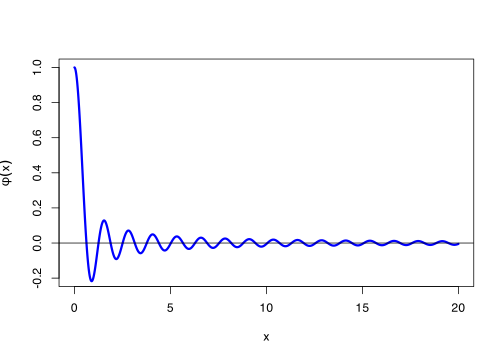
\includegraphics[keepaspectratio]{index_files/mediabag/lectures/L08-is-1_files/figure-pdf/importance-1.pdf}}

We can see that what happens for small \(x\) -- say, for \(x\) between 0
and 2, or so -- will have an important effect on the value of
\(\Exg \phi(X)\), because that where \(\phi\) has the biggest (absolute)
values. But what happens for large \(x\) -- say for \(x \geq 10\) or so
-- will be much less important for estimating \(\Exg\phi(X)\). So it
seems wasteful to have all values in \([0, 20]\) to be sampled equally,
and it would seem to make sense to take more samples from small values
of \(x\).

This is all very well in practice, but how exactly should we down-weight
those over-sampled areas?

Think about estimating \(\Exg \phi(X)\). Let's assume that \(X\) is
continuous with probability density function \(f\). (Throughout this
lecture and the next, we will assume all our random variables are
continuous. The arguments for discrete random variables are very similar
-- just swap probability density functions with probability mass
functions and integrals with sums. You can fill in the details yourself,
if you like.) Then we are trying to estimate
\[ \Exg \phi(X) = \int_{-\infty}^{+\infty} \phi(x)\,f(x)\,\mathrm{d}x = \int_{-\infty}^{+\infty} \phi(y)\,f(y)\,\mathrm{d}y . \]
(In the second equality, we merely changed the ``dummy variable'' from
\(x\) to \(y\), as we are at liberty to do.)

Now suppose we sample from some other continuous distribution \(Y\),
with PDF \(g\). If we estimate \(\Exg \psi(Y)\), say, for some function
\(\psi\), then we are estimating
\[\Exg \psi(Y) = \int_{-\infty}^{+\infty} \psi(y)\,g(y) \, \mathrm{d}y = \int_{-\infty}^{+\infty} \psi(x)\,g(x) \, \mathrm{d}x . \]

But we want to be estimating \(\Exg\phi(X)\), not \(\Exg\psi(Y)\). So we
will need to pick \(\psi\) such that
\[ \Exg \phi(X) = \int_{-\infty}^{+\infty} \phi(y)\,f(y)\,\mathrm{d}y = \int_{-\infty}^{+\infty} \psi(y)\,g(y) \, \mathrm{d}y = \Exg \psi(Y) . \]
So we need to pick \(\psi\) such that \(\phi(y)\,f(y) = \psi(y)\,g(y)\).
That means that we should take
\[\psi(y) = \frac{\phi(y) f(y)}{g(y)} = \frac{f(y)}{g(y)}\,\phi(y). \]

So we could build a Monte Carlo estimate for \(\Exg \phi(X)\) instead as
a Monte Carlo estimate for
\[ \Exg \psi(Y) = \Exg \left(\frac{f(Y)}{g(Y)}\,\phi(Y) \right) . \]

There is one other thing: we need to be careful of division by \(0\)
errors. So we should make sure that \(g\) is only 0 when \(f\) is 0. In
other words, if it's possible for \(X\) to take some value, then it must
be possible for \(Y\) to take that value too.

We are finally ready to define our estimator.

\begin{definition}[]\protect\hypertarget{def-IS}{}\label{def-IS}

Let \(X\) be a continuous random variable with probability density
function \(f\), let \(\phi\) be a function, and write
\(\theta = \Exg\phi(X)\). Let \(Y\) be a continuous random variable with
probability desnity function \(g\), where \(g(y) > 0\) for all \(y\)
where \(f(y) > 0\). Then the \textbf{importance sampling Monte Carlo
estimator} \(\widehat\theta_n^{\mathrm{IS}}\) of \(\theta\) is
\[ \widehat{\theta}_n^{\mathrm{IS}} = \frac{1}{n} \sum_{i=1}^{n} \frac{f(Y_i)}{g(Y_i)}\, \phi(Y_i)   ,\]
where \(Y_1, Y_2, \dots, Y_n\) are independent random samples from
\(Y\).

\end{definition}

We can think of this as taking a weighted mean of the \(\phi(Y_i)\)s,
where the weights are \(f(Y_i)/g(Y_i)\). So if a value \(y\) is more
likely under \(Y\) than under \(X\), then \(g(y)\) is big compared to
\(f(y)\), so \(f(y)/g(y)\) is small, and \(y\) gets a low weight. If a
value \(y\) is less likely under \(Y\) than under \(X\), then \(g(y)\)
is small compared to \(f(y)\), so \(f(y) / g(y)\) is big, and it gets a
high weight. Thus we see that the weighting compensates for values that
are likely to be over- or under-sampled.

\section{Example}\label{example}

\begin{example}[]\protect\hypertarget{exm-IS1}{}\label{exm-IS1}

Let \(X \sim \operatorname{N}(0,1)\) be a standard normal. Suppose we
want to estimate \(\mathbb P(X > 4)\). We could do this the standard
Monte Carlo way by sampling from \(X\) itself.
\[ \widehat{\theta}_n^{\mathrm{MS}} = \frac{1}{n} \sum_{i=1}^n \mathbb I_{[4,\infty)}(X_i) . \]

However, this will not be a good estimator. To see the problem, lets run
this with \(n = 100\,000 = 10^5\) samples, but do it 10 times, and see
what all the estimates are.

\begin{Shaded}
\begin{Highlighting}[]
\NormalTok{n }\OtherTok{\textless{}{-}} \FloatTok{1e5}
\NormalTok{MCest }\OtherTok{\textless{}{-}} \FunctionTok{rep}\NormalTok{(}\DecValTok{0}\NormalTok{, }\DecValTok{10}\NormalTok{)}
\ControlFlowTok{for}\NormalTok{ (i }\ControlFlowTok{in} \DecValTok{1}\SpecialCharTok{:}\DecValTok{10}\NormalTok{) MCest[i] }\OtherTok{\textless{}{-}} \FunctionTok{mean}\NormalTok{(}\FunctionTok{rnorm}\NormalTok{(n) }\SpecialCharTok{\textgreater{}} \DecValTok{4}\NormalTok{)}
\NormalTok{MCest}
\end{Highlighting}
\end{Shaded}

\begin{verbatim}
 [1] 4e-05 3e-05 3e-05 7e-05 1e-05 5e-05 6e-05 1e-05 5e-05 1e-05
\end{verbatim}

We see a big range of values. I get different results each time I run
it, but anything between \(1 \times 10^{-5}\) and \(8 \times 10^{-5}\),
and even \(0\), comes out fairly regularly as the estimate. The problem
is that \(X > 4\) is a very rare event -- it only comes out a handful of
times (perhaps 0 to 8) out of the 100,000 samples. This means our
estimate is (on average) quite inaccurate.

It would be better not to sample from \(X\), but rather to sample from a
distribution that is greater than 4 a better proportion of the time. We
could try anything for this distribution \(Y\), but to keep things
simple, I'm going to stick with a normal distribution with standard
deviation 1. I'll want to increase the mean, though, so that we sample
values bigger than 4 more often. Let's try importance sampling with
\(Y \sim \operatorname{N}(4,1)\).

The PDFs of \(X \sim \operatorname{N}(0,1)\) and
\(Y \sim \operatorname{N}(4,1)\) are
\[f(x) = \frac{1}{\sqrt{2\pi}} \exp\big(-\tfrac12 x^2\big) \qquad g(y) = \frac{1}{\sqrt{2\pi}} \exp\big(-\tfrac12 (y-4)^2\big) , \]
so the relevant weighting of a sample \(y\) is
\[ \frac{f(y)}{g(y)} = \frac{\exp\big(-\tfrac12 y^2\big)}{\exp\big(-\tfrac12 (y-4)^2\big)} = \exp \big(\tfrac12\big(-y^2 + (y-4)^2\big)\big) = \exp(-4y+8) .  \]
So our importance sampling estimate will be
\[ \widehat{\theta}_n^{\mathrm{IS}} = \frac{1}{n} \sum_{i=1}^n \mathrm{e}^{-4Y_i +8} \, \mathbb I_{[4,\infty)}(Y_i) . \]

Let's try this in R. Although we could use the function
\(\mathrm{e}^{-4y+8}\) for the weights, I'll do this by using the ratios
of the PDFs directly in R (just in case I made a mistake\ldots).

\begin{Shaded}
\begin{Highlighting}[]
\NormalTok{n }\OtherTok{\textless{}{-}} \FloatTok{1e5}
\NormalTok{pdf\_x }\OtherTok{\textless{}{-}} \ControlFlowTok{function}\NormalTok{(y) }\FunctionTok{dnorm}\NormalTok{(y, }\DecValTok{0}\NormalTok{, }\DecValTok{1}\NormalTok{)}
\NormalTok{pdf\_y }\OtherTok{\textless{}{-}} \ControlFlowTok{function}\NormalTok{(y) }\FunctionTok{dnorm}\NormalTok{(y, }\DecValTok{4}\NormalTok{, }\DecValTok{1}\NormalTok{)}
\NormalTok{samples\_y }\OtherTok{\textless{}{-}} \FunctionTok{rnorm}\NormalTok{(n, }\DecValTok{4}\NormalTok{, }\DecValTok{1}\NormalTok{)}
\NormalTok{ISest }\OtherTok{\textless{}{-}} \FunctionTok{mean}\NormalTok{((}\FunctionTok{pdf\_x}\NormalTok{(samples\_y) }\SpecialCharTok{/} \FunctionTok{pdf\_y}\NormalTok{(samples\_y)) }\SpecialCharTok{*}\NormalTok{ (samples\_y }\SpecialCharTok{\textgreater{}} \DecValTok{4}\NormalTok{))}
\NormalTok{ISest}
\end{Highlighting}
\end{Shaded}

\begin{verbatim}
[1] 3.163129e-05
\end{verbatim}

\end{example}

\section{Errors in importance
sampling}\label{errors-in-importance-sampling}

The following theorem should not by now be a surprise.

\begin{theorem}[]\protect\hypertarget{thm-Iserr}{}\label{thm-Iserr}

Let \(X\) be a continuous random variable with probability density
function \(f\), let \(\phi\) be a function, and write
\(\theta = \Exg\phi(X)\). Let \(Y\) another continuous random variable
with probability density function with probability density function
\(g\), such that \(g(y) = 0\) only when \(f(y) = 0\). Let
\[ \widehat{\theta}_n^{\mathrm{IS}} = \frac{1}{n} \sum_{i=1}^n \frac{f(Y_i)}{g(Y_i)}\,\phi(Y_i)  \]
be the importance sampling Monte Carlo estimator of \(\theta\). Then:

\begin{enumerate}
\def\labelenumi{\arabic{enumi}.}
\item
  \(\widehat{\theta}_n^{\mathrm{IS}}\) is unbiased, in that
  \(\operatorname{bias}\big(\widehat{\theta}_n^{\mathrm{IS}}\big) = 0\).
\item
  The variance of of \(\widehat{\theta}_n^{\mathrm{IS}}\) is
  \[ \operatorname{Var}\big(\widehat{\theta}_n^{\mathrm{IS}}\big) = \frac{1}{n} \operatorname{Var}\left( \frac{f(Y)}{g(Y)}\,\phi(Y) \right). \]
\item
  The mean-square error of \(\widehat{\theta}_n^{\mathrm{IS}}\) is
  \[ \operatorname{MSE}\big(\widehat{\theta}_n^{\mathrm{IS}}\big) = \frac{1}{n} \operatorname{Var}\left( \frac{f(Y)}{g(Y)}\,\phi(Y) \right) . \]
\item
  The root-mean-square error of \(\widehat{\theta}_n^{\mathrm{IS}}\) is
  \[ \operatorname{RMSE}\big(\widehat{\theta}_n^{\mathrm{IS}}\big) = \frac{1}{\sqrt{n}} \,\sqrt{\operatorname{Var}\left( \frac{f(Y)}{g(Y)}\,\phi(Y) \right)}. \]
\end{enumerate}

\end{theorem}

\begin{proof}
Part 1 follows essentially the same argument as our discussion at the
beginning of this lecture. We have
\[ \Ex \left( \frac{1}{n} \sum_{i=1}^n \frac{f(Y_i)}{g(Y_i)}\,\phi(Y_i) \right) = \frac{1}{n}\, n\, \Ex \left(\frac{f(Y)}{g(Y)}\,\phi(Y)\right) = \Ex \left(\frac{f(Y)}{g(Y)}\,\phi(Y)\right) . \]
But
\[ \Ex \left(\frac{f(Y)}{g(Y)}\,\phi(Y)\right) = \int_{-\infty}^{+\infty} \frac{f(y)}{g(y)}\,\phi(y)\,g(y)\,\mathrm{d}y = \int_{-\infty}^{+\infty} \phi(y) \, f(y) \, \mathrm{d}y = \Exg \phi(X) . \]
This last step is because \(f\) is the PDF of \(X\); it doesn't matter
whether the dummy variable in the integration is \(x\) or \(y\). Hence
the estimator is unbiased.

Parts 2 to 4 follow in the usual way.
\end{proof}

As we are now used to, we can estimate the variance using the sample
variance.

\begin{example}[]\protect\hypertarget{exm-IS2}{}\label{exm-IS2}

We continue Example~\ref{exm-IS1}, where we are estimating
\(\mathbb P(X > 4)\) for \(X \sim \operatorname{N}(0,1)\).

For the standard Monte Carlo method, we estimate the root-mean-square
error as

\begin{Shaded}
\begin{Highlighting}[]
\NormalTok{n }\OtherTok{\textless{}{-}} \FloatTok{1e5}
\NormalTok{MC\_MSE }\OtherTok{\textless{}{-}} \FunctionTok{var}\NormalTok{(}\FunctionTok{rnorm}\NormalTok{(n) }\SpecialCharTok{\textgreater{}} \DecValTok{4}\NormalTok{) }\SpecialCharTok{/}\NormalTok{ n}
\FunctionTok{sqrt}\NormalTok{(MC\_MSE)}
\end{Highlighting}
\end{Shaded}

\begin{verbatim}
[1] 1.732033e-05
\end{verbatim}

As before, this still varies a lot, but it seems to usually be about
\(2 \times 10^{-5}\).

For the importance sampling method, we estimate the mean-square error as

\begin{Shaded}
\begin{Highlighting}[]
\NormalTok{n }\OtherTok{\textless{}{-}} \FloatTok{1e5}
\NormalTok{pdf\_x }\OtherTok{\textless{}{-}} \ControlFlowTok{function}\NormalTok{(x) }\FunctionTok{dnorm}\NormalTok{(x, }\DecValTok{0}\NormalTok{, }\DecValTok{1}\NormalTok{)}
\NormalTok{pdf\_y }\OtherTok{\textless{}{-}} \ControlFlowTok{function}\NormalTok{(y) }\FunctionTok{dnorm}\NormalTok{(y, }\DecValTok{4}\NormalTok{, }\DecValTok{1}\NormalTok{)}
\NormalTok{samples\_y }\OtherTok{\textless{}{-}} \FunctionTok{rnorm}\NormalTok{(n, }\DecValTok{4}\NormalTok{, }\DecValTok{1}\NormalTok{)}
\NormalTok{IS\_MSE }\OtherTok{\textless{}{-}} \FunctionTok{var}\NormalTok{((}\FunctionTok{pdf\_x}\NormalTok{(samples\_y) }\SpecialCharTok{/} \FunctionTok{pdf\_y}\NormalTok{(samples\_y)) }\SpecialCharTok{*}\NormalTok{ (samples\_y }\SpecialCharTok{\textgreater{}} \DecValTok{4}\NormalTok{)) }\SpecialCharTok{/}\NormalTok{ n}
\FunctionTok{sqrt}\NormalTok{(IS\_MSE)}
\end{Highlighting}
\end{Shaded}

\begin{verbatim}
[1] 2.129446e-07
\end{verbatim}

This is about \(2 \times 10^{-7}\). This is about 100 times smaller than
for the standard method: equivalent to taking about 10,000 times as many
samples! That's a huge improvement, which demonstrates the power of
importance sampling.

\end{example}

\textbf{Next time:} \emph{We continue our study of importance sampling
-- and complete our study of Monte Carlo estimation, for now -- by
considering how to pick a good distribution \(Y\).}

\textbf{Summary:}

\begin{itemize}
\item
  Importance sampling estimates \(\Exg \phi(X)\) by sampling from a
  different distribution \(Y\).
\item
  The importance sampling estimator is
  \({\displaystyle \widehat{\theta}_n^{\mathrm{IS}} = \frac{1}{n} \sum_{i=1}^n \frac{f(Y_i)}{g(Y_i)}\,\phi(Y_i)}\).
\item
  The importance sampling estimator is unbiased with mean-square error
  \[ \operatorname{MSE}\big(\widehat{\theta}_n^{\mathrm{IS}}\big) = \frac{1}{n} \operatorname{Var}\left( \frac{f(Y)}{g(Y)}\,\phi(Y) \right) . \]
\end{itemize}

\textbf{\hyperref[solutions]{Solutions}} are now available for Problem
Sheet 1.

\textbf{Read more:}
\href{https://leeds.primo.exlibrisgroup.com/permalink/44LEE_INST/1fj430b/cdi_askewsholts_vlebooks_9781118728031}{Voss,
\emph{An Introduction to Statistical Computing}}, Subsection 3.3.1.

\chapter{Importance sampling II}\label{importance-sampling-ii}

\[ \]

\section{Picking a good distribution}\label{picking-a-good-distribution}

Let's remind ourselves where we've got to on importance sampling.

\begin{itemize}
\item
  We want to estimate \(\Exg \phi(X)\).
\item
  Rather than sampling from \(X\), with PDF \(f\), we instead sample
  from a different distribution \(Y\), with PDF \(g\).
\item
  The estimator is
  \({\displaystyle \widehat\theta_n^{\text{IS}} = \frac{1}{n} \sum_{i=1}^n \frac{f(Y_i)}{g(Y_i)} \, \phi(Y_i) .}\)
\end{itemize}

We've seen that importance sampling can be a very powerful tool, when
used well. But how should pick a good distribution \(Y\) to sample from?

Let's examine the mean-square error more carefully:
\[ \operatorname{MSE}\big(\widehat{\theta}_n^{\mathrm{IS}}\big) = \frac{1}{n} \operatorname{Var}\left( \frac{f(Y)}{g(Y)}\,\phi(Y) \right) . \]
So our goal is to try and pick \(Y\) such that
\(\frac{f(Y)}{g(Y)}\phi(Y)\) has low variance. We also, of course, want
to be able to sample from \(Y\).

The best possible choice, then, would be to pick \(Y\) such that
\(\frac{f(Y)}{g(Y)}\phi(Y)\) is constant -- and therefore has zero
variance! If \(\phi\) is non-negative, then it seems like we should pick
\(Y\) such that its probability density function is
\(g(y) \propto f(y)\phi(y)\). (Here, \(\propto\) is the ``proportional
to'' symbol.) That is, to have \[ g(y) = \frac{1}{Z} f(y)\phi(y) , \]
for some constant \(Z\). Then \(\frac{f(Y)}{g(Y)}\phi(Y) = Z\) is a
constant, has zero variance, and we have a perfect estimator!

What is this constant \(Z\)? Well, \(g\) is a PDF, so it has to
integrate to 1. So we will need to have
\[ 1 = \int_{-\infty}^{+\infty} g(y)\, \mathrm{d}y = \int_{-\infty}^{+\infty} \frac{1}{Z} f(y)\phi(y) \, \mathrm{d}y = \frac{1}{Z} \int_{-\infty}^{+\infty} f(x)\phi(x) \, \mathrm{d}x = \frac{1}{Z} \Exg\phi(X) . \]
(We did the ``switching the dummy variable from \(y\) to \(x\)'' thing
again.) So \(Z = \Exg \phi(X)\). But that's no good:
\(\theta = \Exg \phi(X)\) was the thing we were trying to estimate in
the first place. If we knew that, we wouldn't have to do Monte Carlo
estimation to start with!

So, as much as we would like to, we can't use this ``perfect'' ideal
distribution \(Y\). More generally, if \(\phi\) is not always
non-negative, it can be shown that
\(g(y) \propto f(y)\,|\phi(y)| = |f(x)\,\phi(x)|\) would be the best
possible distribution, but this has the same problems.

However, we can still be guided by this idea -- we would like \(g(y)\)
to be as close to proportional to \(f(y) \phi(y)\) (or
\(|f(y) \phi(y)|\)) as we can manage, so that
\(\frac{f(y)}{g(y)}\phi(y)\) is close to being constant, so hopefully
has low variance. This tells us that \(Y\) should be likely -- that is,
\(g(y)\) should be big -- where both \(f\) and \(|\phi|\) are both big
-- that is, where \(X\) is likely and also \(\phi\) is big in absolute
value. While \(Y\) should be unlikely where both \(X\) is unlikely and
\(\phi\) is small in absolute value.

\begin{example}[]\protect\hypertarget{exm-IS3}{}\label{exm-IS3}

Let's look again at Example~\ref{exm-IS1} (continued in
Example~\ref{exm-IS2}), where we wanted to estimate
\(\mathbb P(X > 4) = \Exg\Ind_{(4,\infty)}(X)\) for
\(X \sim \operatorname{N}(0,1)\). We found are estimator was enormously
improved when we used instead \(Y \sim \operatorname{N}(4,1)\).

In the figure below, the blue line is
\[f(y)\,\phi(y) = f(y)\,\Ind_{(4,\infty)}(y) = \begin{cases} \displaystyle\frac{1}{\sqrt{2\pi}} \,\mathrm{e}^{-y^2/2} & y > 4 \\ 0 & y \leq 4 \end{cases} \]
(scaled up, otherwise it would be so close to the axis line you wouldn't
see it).

The black line is the PDF \(f(y)\) of the original distribution
\(X \sim \operatorname{N}(0,1)\), while the red line is the PDF \(g(y)\)
of our importance distribution \(Y \sim \operatorname{N}(4,1)\).

\begin{Shaded}
\begin{Highlighting}[]
\FunctionTok{curve}\NormalTok{(}
  \FunctionTok{dnorm}\NormalTok{(x, }\DecValTok{0}\NormalTok{, }\DecValTok{1}\NormalTok{), }\AttributeTok{n =} \DecValTok{1001}\NormalTok{, }\AttributeTok{from =} \SpecialCharTok{{-}}\FloatTok{2.5}\NormalTok{, }\AttributeTok{to =} \FloatTok{7.5}\NormalTok{,}
  \AttributeTok{col =} \StringTok{"black"}\NormalTok{, }\AttributeTok{lwd =} \DecValTok{2}\NormalTok{,}
  \AttributeTok{xlim =} \FunctionTok{c}\NormalTok{(}\SpecialCharTok{{-}}\DecValTok{2}\NormalTok{, }\DecValTok{7}\NormalTok{), }\AttributeTok{xlab =} \StringTok{"y"}\NormalTok{, }\AttributeTok{ylim =} \FunctionTok{c}\NormalTok{(}\DecValTok{0}\NormalTok{, }\FloatTok{0.7}\NormalTok{), }\AttributeTok{ylab =} \StringTok{""}
\NormalTok{)}
\FunctionTok{curve}\NormalTok{(}
  \FunctionTok{dnorm}\NormalTok{(x, }\DecValTok{4}\NormalTok{, }\DecValTok{1}\NormalTok{), }\AttributeTok{n =} \DecValTok{1001}\NormalTok{, }\AttributeTok{from =} \SpecialCharTok{{-}}\FloatTok{2.5}\NormalTok{, }\AttributeTok{to =} \FloatTok{7.5}\NormalTok{,}
  \AttributeTok{add =} \ConstantTok{TRUE}\NormalTok{, }\AttributeTok{col =} \StringTok{"red"}\NormalTok{, }\AttributeTok{lwd =} \DecValTok{3}\NormalTok{,}
\NormalTok{)}
\FunctionTok{curve}\NormalTok{(}
  \FunctionTok{dnorm}\NormalTok{(x, }\DecValTok{0}\NormalTok{, }\DecValTok{1}\NormalTok{) }\SpecialCharTok{*}\NormalTok{ (x }\SpecialCharTok{\textgreater{}} \DecValTok{4}\NormalTok{) }\SpecialCharTok{*} \DecValTok{5000}\NormalTok{, }\AttributeTok{n =} \DecValTok{1001}\NormalTok{, }\AttributeTok{from =} \SpecialCharTok{{-}}\FloatTok{2.5}\NormalTok{, }\AttributeTok{to =} \FloatTok{7.5}\NormalTok{,}
  \AttributeTok{add =} \ConstantTok{TRUE}\NormalTok{, }\AttributeTok{col =} \StringTok{"blue"}\NormalTok{, }\AttributeTok{lwd =} \DecValTok{3}
\NormalTok{)}
\FunctionTok{legend}\NormalTok{(}
  \StringTok{"topright"}\NormalTok{,}
  \FunctionTok{c}\NormalTok{(}\FunctionTok{expression}\NormalTok{(}\FunctionTok{paste}\NormalTok{(}\StringTok{"f(y)"}\NormalTok{, varphi, }\StringTok{"(y) [scaled]"}\NormalTok{)), }\StringTok{"N(0, 1)"}\NormalTok{, }\StringTok{"N(4, 1)"}\NormalTok{),}
  \AttributeTok{lwd =} \FunctionTok{c}\NormalTok{(}\DecValTok{3}\NormalTok{, }\DecValTok{2}\NormalTok{, }\DecValTok{3}\NormalTok{), }\AttributeTok{col =} \FunctionTok{c}\NormalTok{(}\StringTok{"blue"}\NormalTok{, }\StringTok{"black"}\NormalTok{, }\StringTok{"red"}\NormalTok{)}
\NormalTok{)}
\end{Highlighting}
\end{Shaded}

\pandocbounded{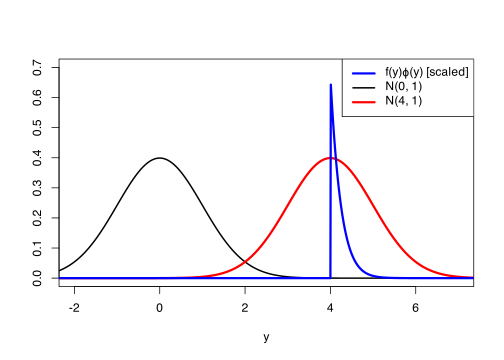
\includegraphics[keepaspectratio]{index_files/mediabag/lectures/L09-is-2_files/figure-pdf/propto-1.pdf}}

We have noted that a good distribution will have a PDF that is big when
\(f(x)\phi(x)\) (the blue line) is big. Clearly the red line is much
better at this then the black line, which is why the importance sampling
method was so much better here.

There's scope to do better here, though. Perhaps an asymmetric
distribution with a much more quickly-decaying left-tail might be good
-- for example, a shifted exponential
\(4 + \operatorname{Exp}(\lambda)\) might be worth investigating. Or a
thinner, spikier distribution, such as a normal with smaller standard
deviation. In both cases, though, we have to be careful -- because it's
the ratio \(f(y)/g(y)\), we still have to be a bit careful about what
happens when both \(f(y)\) and \(g(y)\) are small \emph{absolutely}, in
case one is \emph{proportionally} much bigger than the other.

\end{example}

Aside from the exact theory, in the absence of any better idea, choosing
\(Y\) to be ``in the same distribution family as \(X\) but with
different parameters'' is often a reasonable thing to try. For example:

\begin{itemize}
\item
  If \(X \sim \operatorname{N}(\mu, \sigma^2)\), then try
  \(Y \sim \operatorname{N}(\nu, \sigma^2)\) for some other value
  \(\nu\).
\item
  If \(X \sim \operatorname{Exp}(\lambda)\), then try
  \(Y \sim \operatorname{Exp}(\mu)\) for some other value \(\mu\).
\end{itemize}

\section{Bonus example}\label{bonus-example}

\begin{example}[]\protect\hypertarget{exm-ISnew}{}\label{exm-ISnew}

\emph{Let} \(X \sim \operatorname{U}[0, 10]\) be an uniform
distribution, so \(f(x) = \frac{1}{10}\) for \(0 \leq x \leq 10\), and
let \(\phi(x) = \mathrm{e}^{-|x-8|}\). Estimate \(\Exg\phi(X)\).

The standard Monte Carlo estimator and its RMSE are as follows

\begin{Shaded}
\begin{Highlighting}[]
\NormalTok{phi }\OtherTok{\textless{}{-}} \ControlFlowTok{function}\NormalTok{(x) }\FunctionTok{exp}\NormalTok{(}\SpecialCharTok{{-}}\FunctionTok{abs}\NormalTok{(x }\SpecialCharTok{{-}} \DecValTok{8}\NormalTok{))}
\NormalTok{n }\OtherTok{\textless{}{-}} \FloatTok{1e6}
\NormalTok{samples }\OtherTok{\textless{}{-}} \FunctionTok{runif}\NormalTok{(n, }\DecValTok{0}\NormalTok{, }\DecValTok{10}\NormalTok{)}
\NormalTok{MCest }\OtherTok{\textless{}{-}} \FunctionTok{mean}\NormalTok{(}\FunctionTok{phi}\NormalTok{(samples))}
\NormalTok{MC\_MSE }\OtherTok{\textless{}{-}} \FunctionTok{var}\NormalTok{(}\FunctionTok{phi}\NormalTok{(samples)) }\SpecialCharTok{/}\NormalTok{ n}
\FunctionTok{c}\NormalTok{(MCest, }\FunctionTok{sqrt}\NormalTok{(MC\_MSE))}
\end{Highlighting}
\end{Shaded}

\begin{verbatim}
[1] 0.1865579341 0.0002537701
\end{verbatim}

Maybe we can improve on this using importance sampling. Let's have a
look at a graph of \(f(y)\,\phi(y)\) (blue line).

\begin{Shaded}
\begin{Highlighting}[]
\FunctionTok{curve}\NormalTok{(}
  \FunctionTok{dunif}\NormalTok{(x, }\DecValTok{0}\NormalTok{, }\DecValTok{10}\NormalTok{) }\SpecialCharTok{*} \FunctionTok{exp}\NormalTok{(}\SpecialCharTok{{-}}\FunctionTok{abs}\NormalTok{(x }\SpecialCharTok{{-}} \DecValTok{8}\NormalTok{)), }\AttributeTok{n =} \DecValTok{1001}\NormalTok{, }\AttributeTok{from =} \SpecialCharTok{{-}}\DecValTok{1}\NormalTok{, }\AttributeTok{to =} \DecValTok{11}\NormalTok{,}
  \AttributeTok{col =} \StringTok{"blue"}\NormalTok{, }\AttributeTok{lwd =} \DecValTok{3}\NormalTok{,}
  \AttributeTok{xlim =} \FunctionTok{c}\NormalTok{(}\DecValTok{0}\NormalTok{, }\DecValTok{10}\NormalTok{), }\AttributeTok{xlab =} \StringTok{"y"}\NormalTok{, }\AttributeTok{ylab =} \StringTok{""}
\NormalTok{)}
\FunctionTok{curve}\NormalTok{(}
  \FunctionTok{dnorm}\NormalTok{(x, }\DecValTok{8}\NormalTok{, }\DecValTok{2}\NormalTok{)}\SpecialCharTok{*}\FloatTok{0.36}\NormalTok{, }\AttributeTok{n =} \DecValTok{1001}\NormalTok{, }\AttributeTok{from =} \SpecialCharTok{{-}}\DecValTok{1}\NormalTok{, }\AttributeTok{to =} \DecValTok{11}\NormalTok{,}
  \AttributeTok{add =} \ConstantTok{TRUE}\NormalTok{, }\AttributeTok{col =} \StringTok{"red"}\NormalTok{, }\AttributeTok{lwd =} \DecValTok{2}\NormalTok{,}
\NormalTok{)}
\FunctionTok{legend}\NormalTok{(}
  \StringTok{"topleft"}\NormalTok{,}
  \FunctionTok{c}\NormalTok{(}\FunctionTok{expression}\NormalTok{(}\FunctionTok{paste}\NormalTok{(}\StringTok{"f(y)"}\NormalTok{, varphi, }\StringTok{"(y)"}\NormalTok{)), }\StringTok{"N(8, 4) [scaled]"}\NormalTok{),}
  \AttributeTok{lwd =} \FunctionTok{c}\NormalTok{(}\DecValTok{3}\NormalTok{, }\DecValTok{2}\NormalTok{), }\AttributeTok{col =} \FunctionTok{c}\NormalTok{(}\StringTok{"blue"}\NormalTok{, }\StringTok{"red"}\NormalTok{)}
\NormalTok{)}
\end{Highlighting}
\end{Shaded}

\pandocbounded{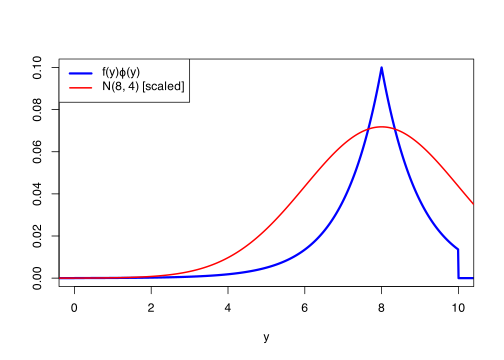
\includegraphics[keepaspectratio]{index_files/mediabag/lectures/L09-is-2_files/figure-pdf/propto2-1.pdf}}

After some experimentation, I decided that
\(Y \sim \operatorname{N}(8, 2^2)\) (red line; not to same scale) seemed
to work quite well, in \(g(y)\) being roughly proportional to
\(f(y)\,\phi(y)\). (Maybe reducing the standard deviation a bit more, to
around 1.6, to get the red curve a bit tighter, might have done a little
bit better still.)

The following graph shows \(\frac{f(y)}{g(y)} \phi(y)\), and shows that
the graph is not \emph{too} pointy, so should have reasonably small
variance.

\begin{Shaded}
\begin{Highlighting}[]
\FunctionTok{curve}\NormalTok{(}
  \FunctionTok{dunif}\NormalTok{(x, }\DecValTok{0}\NormalTok{, }\DecValTok{10}\NormalTok{) }\SpecialCharTok{*} \FunctionTok{exp}\NormalTok{(}\SpecialCharTok{{-}}\FunctionTok{abs}\NormalTok{(x }\SpecialCharTok{{-}} \DecValTok{8}\NormalTok{)) }\SpecialCharTok{/} \FunctionTok{dnorm}\NormalTok{(x, }\DecValTok{8}\NormalTok{, }\DecValTok{2}\NormalTok{), }\AttributeTok{n =} \DecValTok{1001}\NormalTok{, }\AttributeTok{from =} \SpecialCharTok{{-}}\DecValTok{2}\NormalTok{, }\AttributeTok{to =} \DecValTok{12}\NormalTok{,}
  \AttributeTok{col =} \StringTok{"red"}\NormalTok{, }\AttributeTok{lwd =} \DecValTok{3}\NormalTok{,}
  \AttributeTok{xlim =} \FunctionTok{c}\NormalTok{(}\SpecialCharTok{{-}}\DecValTok{1}\NormalTok{, }\DecValTok{11}\NormalTok{), }\AttributeTok{xlab =} \StringTok{"y"}\NormalTok{, }\AttributeTok{ylab =} \StringTok{""}
\NormalTok{)}
\end{Highlighting}
\end{Shaded}

\pandocbounded{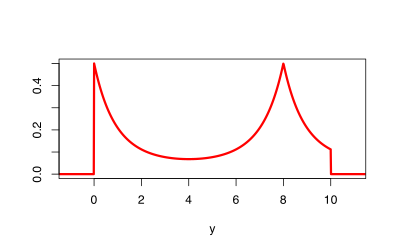
\includegraphics[keepaspectratio]{index_files/mediabag/lectures/L09-is-2_files/figure-pdf/propto3-1.pdf}}

So our importance sampling estimate is as follows.

\begin{Shaded}
\begin{Highlighting}[]
\NormalTok{phi }\OtherTok{\textless{}{-}} \ControlFlowTok{function}\NormalTok{(x) }\FunctionTok{exp}\NormalTok{(}\SpecialCharTok{{-}}\FunctionTok{abs}\NormalTok{(x }\SpecialCharTok{{-}} \DecValTok{8}\NormalTok{))}
\NormalTok{pdf\_x }\OtherTok{\textless{}{-}} \ControlFlowTok{function}\NormalTok{(x) }\FunctionTok{dunif}\NormalTok{(x, }\DecValTok{0}\NormalTok{, }\DecValTok{10}\NormalTok{)}
\NormalTok{pdf\_y }\OtherTok{\textless{}{-}} \ControlFlowTok{function}\NormalTok{(y) }\FunctionTok{dnorm}\NormalTok{(y, }\DecValTok{8}\NormalTok{, }\DecValTok{2}\NormalTok{)}

\NormalTok{n }\OtherTok{\textless{}{-}} \FloatTok{1e6}
\NormalTok{samples }\OtherTok{\textless{}{-}} \FunctionTok{rnorm}\NormalTok{(n, }\DecValTok{8}\NormalTok{, }\DecValTok{2}\NormalTok{)}
\NormalTok{ISest }\OtherTok{\textless{}{-}} \FunctionTok{mean}\NormalTok{((}\FunctionTok{pdf\_x}\NormalTok{(samples) }\SpecialCharTok{/} \FunctionTok{pdf\_y}\NormalTok{(samples)) }\SpecialCharTok{*} \FunctionTok{phi}\NormalTok{(samples))}
\NormalTok{IS\_MSE }\OtherTok{\textless{}{-}} \FunctionTok{var}\NormalTok{((}\FunctionTok{pdf\_x}\NormalTok{(samples) }\SpecialCharTok{/} \FunctionTok{pdf\_y}\NormalTok{(samples)) }\SpecialCharTok{*} \FunctionTok{phi}\NormalTok{(samples)) }\SpecialCharTok{/}\NormalTok{ n}
\FunctionTok{c}\NormalTok{(ISest, }\FunctionTok{sqrt}\NormalTok{(IS\_MSE))}
\end{Highlighting}
\end{Shaded}

\begin{verbatim}
[1] 0.1863512119 0.0001351446
\end{verbatim}

We see that the RMSE has roughly halved, which is the equivalent of
taking four times as many samples.

\end{example}

\section{Summary of Part I}\label{summary-of-part-i}

This is our last lecture on Monte Carlo estimation -- at least for now,
and at least in its standard form. So let's end this section of the
module by summarising the estimators we have learned about. We have been
learning how to estimate \(\theta = \Exg \phi(X)\)

\begin{itemize}
\item
  The \textbf{standard Monte Carlo estimator} simple takes a sample mean
  of \(\phi(X_i)\), where \(X_i\) are independent random samples from
  \(X\).
\item
  The \textbf{control variate} Monte Carlo estimator ``anchors'' the
  estimator to some known value \(\eta = \Exg \psi(X)\), for a function
  \(\psi\) that is ``similar to \(\phi\), but easier to calculate the
  expectation exactly''.
\item
  The \textbf{antithetic variables} Monte Carlo estimator uses pairs of
  samples \((X_i, X'_i)\) that both have the same distribution as \(X\),
  but where \(\phi(X)\) and \(\phi(X')\) have negative correlation
  \(\rho < 0\).
\item
  The \textbf{importance sampling} Monte Carlo estimator samples not
  from \(X\), with PDF \(f\), but from a different distribution \(Y\),
  with PDF \(Y\). The distribution \(Y\) is chosen to oversample from
  the most important values, but then gives lower weight to those
  samples.
\end{itemize}

\begin{longtable}[]{@{}
  >{\centering\arraybackslash}p{(\linewidth - 4\tabcolsep) * \real{0.3333}}
  >{\centering\arraybackslash}p{(\linewidth - 4\tabcolsep) * \real{0.3333}}
  >{\centering\arraybackslash}p{(\linewidth - 4\tabcolsep) * \real{0.3333}}@{}}
\toprule\noalign{}
\begin{minipage}[b]{\linewidth}\centering
\end{minipage} & \begin{minipage}[b]{\linewidth}\centering
\textbf{Estimator}
\end{minipage} & \begin{minipage}[b]{\linewidth}\centering
\textbf{MSE}
\end{minipage} \\
\midrule\noalign{}
\endhead
\bottomrule\noalign{}
\endlastfoot
\textbf{Standard Monte Carlo} &
\({\displaystyle\frac{1}{n} \sum_{i=1}^n \phi(X_i)}\) &
\({\displaystyle\frac{1}{n} \operatorname{Var}\big(\phi(X)\big)}\) \\
\textbf{Control variate} &
\({\displaystyle\frac{1}{n} \sum_{i=1}^n \big(\phi(X_i) - \psi(X_i)\big)} + \eta\)
&
\({\displaystyle\frac{1}{n} \operatorname{Var}\big(\phi(X_i) - \psi(X_i)\big)}\) \\
\textbf{Antithetic variables} &
\({\displaystyle\frac{1}{n} \sum_{i=1}^{n/2} \big(\phi(X_i) + \phi(X_i')\big)}\)
&
\({\displaystyle\frac{1}{2n} \operatorname{Var}\big(\phi(X_i) + \phi(X_i')\big)}\)
\({\displaystyle {}= \frac{1+\rho}{n} \,\operatorname{Var}\big(\phi(X)\big)}\) \\
\textbf{Importance sampling} &
\({\displaystyle\frac{1}{n} \sum_{i=1}^n \frac{f(Y_i)}{g(Y_i)}\,\phi(X_i)}\)
&
\({\displaystyle\frac{1}{n} \operatorname{Var}\left(\frac{f(Y_i)}{g(Y_i)}\,\phi(X_i)\right)}\) \\
\end{longtable}

~

\textbf{Next time:} \emph{We begin the second section of the module, on
random number generation.}

\textbf{Summary:}

\begin{itemize}
\tightlist
\item
  A good importance sampling distribution \(Y\) is one whose PDF
  \(g(y)\) is roughly proportional to \(|f(y)\,\phi(y)|\). Equivalently,
  \(\frac{f(y)}{g(y)}|\phi(y)|\) is approximately constant.
\end{itemize}

You should now be able to answer Questions 1--3 on
\hyperref[P2]{\textbf{Problem Sheet 2}}.

\textbf{Read more:}
\href{https://leeds.primo.exlibrisgroup.com/permalink/44LEE_INST/1fj430b/cdi_askewsholts_vlebooks_9781118728031}{Voss,
\emph{An Introduction to Statistical Computing}}, Subsection 3.3.1.

\part{Random number generation}

\chapter{Generating random numbers}\label{generating-random-numbers}

Please complete the
\href{https://forms.office.com/e/T1s1md6Jxi}{\textbf{mid-semester
survey}}.

\section{Why generate random
numbers?}\label{why-generate-random-numbers}

So far in this module, we have made a lot of use of generating random
numbers or random samples -- for us, this has been when performing Monte
Carlo estimation. We will also need random numbers for other purposes
later in the module. There are lots of other situations in statistics,
mathematics, data science, physics, computer science, cryptography,
\ldots{} where we want to use random numbers to help us solve problems.
But where do we get these random numbers from?

When performing Monte Carlo estimation, we have used lots of samples
from the distribution of some random variable \(X\). We did this using
R's built-in functions for random number generation, like
\texttt{runif()}, \texttt{rnorm()}, \texttt{rexp()}, and so on.

In this part of the module, we are interested in these questions:

\begin{itemize}
\item
  How do these random number generation functions in R actually
  \emph{work}?
\item
  What if we want to sample from a distribution for which R doesn't have
  a built-in function -- how can we do that?
\end{itemize}

It turns out that this will break down into two questions that we can
treat largely separately:

\begin{enumerate}
\def\labelenumi{\arabic{enumi}.}
\item
  How do we generate some randomness -- any randomness -- in the first
  place? We usually think of this as generating
  \(U \sim \operatorname{U}[0,1]\), a uniform random number between 0
  and 1. (We will look at this today and in the next lecture.)
\item
  How do we transform that uniform randomness \(U\) to get it to behave
  like the particular distribution \(X\) that we want to sample from?
  (We will look at this in Lectures 12--16.)
\end{enumerate}

\section{Random numbers on computers}\label{random-numbers-on-computers}

We start by considering the question of how to generate a uniform random
number between 0 and 1.

The first thing to know is that computers do not perfectly store exact
real numbers in decimals of unending length -- that's impossible!
Instead, it stores a number to a certain accuracy, in terms of the
number of decimal places. To be more precise, computers store numbers in
\emph{binary}; that is, written as a sequence of 0s and 1s. These 0s and
1s are called ``binary digits'', or \textbf{bits}, for short. (In the
presentation here, we will somewhat simplify matters -- computer science
experts will be able to spot where I'm lying, or ``gently smoothing out
the truth''.)

A number between 0 and 1 could be (approximately) stored as a 32-bit
binary number, for example. A 32-bit number is a number like

\begin{verbatim}
0. 00110100 11110100 10001111 10011001
\end{verbatim}

that is ``0.'' followed by a string of 32 binary digits. A string
\(0.x_1x_2\cdots x_{31}x_{32}\) represents the number
\[ x = \sum_{i=1}^{32} x_i 2^{-i} . \] So the number above represents
\begin{align} &0\times 2^{-1} + 0 \times 2^{-2} + 1 \times 2^{-3} + \cdots + 0 \times 2^{-31} + 1 \times 2^{-32} \\ &\qquad\qquad {}=2^{-3} + 2^{-4} + 2^{-6} + \dots + 2^{-29} + 2^{-32} \\ &\qquad\qquad {}= 0.20685670361854135990142822265625.\end{align}

We could generate such a 32-bit (or, more generally, \(b\)-bit) number
in two different ways:

\begin{itemize}
\tightlist
\item
  A sequence of 32 0s and 1s (each being 50:50 likely to be 0 or 1 and
  each being independent of the others). This then represents a number
  in its binary expansion, as above.

  \begin{itemize}
  \tightlist
  \item
    Or, more generally, we want a string of \(b\) 0s and 1s.
  \end{itemize}
\item
  A integer at random between \(0\) and \(2^{32} - 1\), which we can
  then divide by \(2^{32}\) to get a number between \(0\) and \(1\).

  \begin{itemize}
  \tightlist
  \item
    Or, more generally, we want a random integer between \(0\) and
    \(m - 1\) for some \(m\), which we can then divide by \(m\). Usually
    \(m = 2^b\) for some \(b\), to give a \(b\)-bit number.
  \end{itemize}
\end{itemize}

There are two ways we can do this. First, we can use \textbf{true
physical randomness}. Second, we can use \textbf{computer-generated
``pseudorandomness''}.

True physical randomness means randomness from some real-life random
process. For example, you could toss a coin 32 times, and write down
``1'' each time it lands heads and ``0'' each time it lands tails: this
would give a random 32-bit number. While this will be genuinely random,
it is, of course, very slow if you need a large amount of randomness.
For example, when we have done Monte Carlo estimation, we have often
used one million random numbers, which took R about 1 second -- it's
obviously completely infeasible to toss 32 million coins that quickly!

For a greater amount of physical randomness more quickly, one could look
at times between the decay of radioactive particles, thermal noise in
electrical circuits, the behaviour of photons in a laser beam, and so
on. But these are quite expensive, and even these may not be quick
enough for some applications.

The bad news about true physical randomness is that it is typically slow
and expensive. But the good news is that we know it will definitely be
perfectly random with no hidden patterns. (For Monte Carlo, we probably
are happy simply to avoid any ``obvious'' patterns; but for uses in
cryptography, for example, true perfect randomness ensuring no patterns
that an enemy could exploit can be very important.)

Here's a cool video by the YouTuber
\href{https://www.youtube.com/@TomScottGo}{Tom Scott} about an internet
company that uses a wall of lava lamps for their true physical
randomness:

\url{https://www.youtube.com/embed/1cUUfMeOijg}

\section{PRNGs}\label{prngs}

A \textbf{pseudorandom number generator} (\textbf{PRNG}) is a computer
program that outputs a sequence of numbers that appear to be random. Of
course, the numbers are not \emph{actually} random -- a computer program
always performs exactly what you tell it to, exactly the same every
time. But for a PRNG -- or at least for a good PRNG -- there should be
no obvious patterns in the sequence of numbers produced, so they should
act for all practical purposes \emph{as if} they were random numbers.
(``Pseudo'' is a prefix that means something like ``appears to be, even
though it's not''.) The best thing about PRNGs is because they are
simple computer programs they run very very quickly and cheaply.

Many pseudorandom number generators work by applying a
\textbf{recurrence}; that is, applying a function again and again.
Suppose we want (pseudo)random integers between \(0\) and \(m-1\). Then
we have a \textbf{seed} \(x_1\), which behaves as a starting point for
the sequence, and a function \(f\) from \(\{0, 1, \dots, m-1\}\) to
\(\{0, 1, \dots, m-1\}\). Then starting from \(x_1\), we apply \(f\) to
get the next number in the sequence \(x_2 = f(x_1)\). Then we apply
\(f\) to \emph{that}, to get the next point \(x_3 = f(x_2)\). Then apply
\(f\) to \emph{that} to get the next number, and so on. So the sequence
would be
\begin{align} x_1& & x_2 &= f(x_1) & x_3 &= f(x_2) = f(f(x_1)) \\
x_4 &= f(x_3) = f(f(f(x_1))) & &\cdots & x_{i+1} &= f(x_i) =f(f(\cdots (f(x_1))\cdots))\end{align}
and so on.

Some functions \(f\) would be not produce a very random-looking sequence
of numbers: think of a silly example like \(f(x) = (x+1) \bmod m\), so
\(x_{i+1} = (x_i + 1) \bmod m\) just increases by 1 each time, before
``wrapping around'' back to 0 when it gets to \(m\). (The ``mod \(m\)''
means to wrap around when you get to \(m\), or to take the remainder
when you divide by \(m\).) But mathematicians have come up with lots of
examples of functions \(f\) which, for all possible practical purposes,
seem to have outputs that appear just as random as an actual random
sequence.

One example of such a function \(f\) would be \(f(x) = (ax+c) \bmod m\),
so \(x_{i+1} = (ax_i + c)\bmod m\), which can be a very good PRNG for
some values of \(a\) and \(c\). In this case, the PRNG is known as a
\textbf{linear congruential generator} (or \textbf{LCG}). We'll talk
more about LCGs in the next lecture.

R's default method is of this form -- well, it's \emph{almost} a
recurrence of the form \(x_{i+1} = f(x_i)\). It actually uses a method
called the
\href{https://en.wikipedia.org/wiki/Mersenne_Twister}{Mersenne Twister},
which uses a recurrence of the form \(x_{i+1} = (g(x_i) + i) \bmod m\)
for a complicated function \(g\); here the ``plus \(i\)'', where \(i\)
is the step number, means we have a slightly different update rule each
timestep.

But how do we pick the seed -- the starting point \(x_1\)? Normally, we
use some true physical randomness to pick the seed. The benefit here is
that just a small amount of true physical randomness can ``start you
off'' by choosing the seed, and then the PRNG can produces huge amounts
of pseudorandomness incredibly quickly. Indeed, that's what the wall of
lava lamps in the video did -- the lava lamps were just for producing
lots of seeds for the PRNGs.

However, it is possible, and sometimes desirable, to set the seed ``by
hand''. This is useful if you want to produce the same
``random-looking'' numbers as someone else (or yourself, previously).
This is because if two people set the same seed \(x_1\), then the
numbers \(x_2, x_3, \dots\) produced after that will still appear to be
random, but because the process is completely deterministic after the
seed is chosen, both people will actually produce exactly the same
sequence of numbers. This can be useful for checking accuracy of code,
for example, or ensuring ``reproducible analysis''.

In R, by default, the seed is set based the current time on your
computer, measured down to about 10 milliseconds. However, you can set
the seed yourself, using \texttt{set.seed()}. For example, the following
code sets the seed to be 123456, then generates 10 uniform pseudorandom
numbers.

\begin{Shaded}
\begin{Highlighting}[]
\FunctionTok{set.seed}\NormalTok{(}\DecValTok{123456}\NormalTok{)}
\FunctionTok{runif}\NormalTok{(}\DecValTok{10}\NormalTok{)}
\end{Highlighting}
\end{Shaded}

\begin{verbatim}
 [1] 0.79778432 0.75356509 0.39125568 0.34155670 0.36129411 0.19834473
 [7] 0.53485796 0.09652624 0.98784694 0.16756948
\end{verbatim}

Those numbers certainly appear to be random. But if you run those two
lines of code on your computer, you should get exactly the same 10
numbers that I got. That's because you will also start with the same
seed 123456, and then R will run the same pseudorandom -- that is,
completely deterministic -- function to generate the next 10 numbers.

So PRNGs are quick and cheap. If they are designed well and started from
a truly random seed, then we hope there will be know hidden patterns in
the numbers, although it is difficult to be sure.

\textbf{Next time:} \emph{We'll take a closer look at pseudorandom
number generation using linear congruential generators.}

\textbf{Summary:}

\begin{itemize}
\item
  Random number generation has two problems: how to generate uniform
  random numbers between 0 and 1, and how to convert these to your
  desired distribution.
\item
  Uniform random numbers can be generated from true physical randomness
  (which will definitely be totally random, but will be slow and
  expensive) or using a pseudorandom number generator on a computer
  (which is very fast, but needs to be designed carefully to ensure a
  random-looking output).
\item
  LCGs are a type of pseudorandom number generator that are started from
  a ``seed'', which can be chosen using physical randomness or set by
  the user.
\end{itemize}

\textbf{Read more:}
\href{https://leeds.primo.exlibrisgroup.com/permalink/44LEE_INST/1fj430b/cdi_askewsholts_vlebooks_9781118728031}{Voss,
\emph{An Introduction to Statistical Computing}}, introduction to
Chapter 1, introduction to Section 1.1, and Subsection 1.1.3.

\chapter{LCGs}\label{lcgs}

\section{Definition and examples}\label{definition-and-examples}

Last lecture we introduced the idea of pseudorandom number generators
(PRNGs), which are deterministic functions that produce a sequence of
numbers that look for all practical purposes as if they are random.

We introduced the idea of a recurrence, where we have a function \(f\)
and start with a seed \(x_1\). We then produce a sequence through the
recurrence \(x_{i+1} = f(x_i)\). So \(x_2 = f(x_1)\),
\(x_3 = f(x_2) = f(f(x_1))\), and so on.

We briefly mentioned a class of such PRNGs called \textbf{linear
congruential generators}, or \textbf{LCGs}. An LCG generates integers
between \(0\) and \(m-1\) using a recurrence function of the form
\[ f(x) = (ax + c) \bmod m , \] so \[ x_{i+1} = (ax_i + c) \bmod m . \]

Here, ``\(\mathrm{mod}\ m\)'' means ``modulo \(m\)''; that is, we are
using modular arithmetic, where when we get to \(m - 1\) we wrap back to
0 and start again. (Modular arithmetic is sometimes called ``clock
arithmetic'', because hours of the day work modulo 12: for example, 3
hours after 11 o'clock is 2 o'clock, because
\(11 + 3 = 14 \equiv 2 \bmod m\).)

In the LCG \(x_{i+1} = (ax_i + c) \bmod m\):

\begin{itemize}
\item
  \(m\) is called the \textbf{modulus},
\item
  \(a\) is called the \textbf{multiplier},
\item
  \(c\) is called the \textbf{increment},
\item
  \(x_1\), the starting point, is called the \textbf{seed}.
\end{itemize}

\begin{example}[]\protect\hypertarget{exm-lcg-easy}{}\label{exm-lcg-easy}

Let us look at two simple LCGs with modulus \(m = 2^4 = 16\).

First, let \(a = 5\) be the multiplier, \(c = 3\) be the increment, and
\(x_1 = 1\) be the seed. Then we have
\begin{align} x_2 &= (5x_1 + 3) \bmod 16 = (5\times 1 + 3) \bmod 16 = 8 \bmod 16 = 8 \\
x_3 &= (5x_2 + 3) \bmod 16 = (5\times 8 + 3) \bmod 16 = 43 \bmod 16 = 11 \\
x_4 &= (5x_3 + 3) \bmod 16 = (5\times 1 + 3) \bmod 16 = 43 \bmod 58 = 10 , \end{align}
and so on. The sequence continues
\((1, 8, 11, 10, 5, 12, 15, 14, 9, 0, \dots)\). This looks pretty much
like a random sequence of numbers between 0 and 15 to me -- I certainly
don't see any obvious pattern.

Second, let \(a = 3\) be the multiplier, \(c = 6\) be the increment, and
\(x_1 = 1\) be the seed. Then we have
\begin{align} x_2 &= (3x_1 + 2) \bmod 16 = (3\times 1 + 6) \bmod 16 = 9 \bmod 16 = 9 \\
x_3 &= (3x_2 + 4) \bmod 16 = (3\times 9 + 6) \bmod 16 = 33 \bmod 16 = 1 . \end{align}
But now, using \(x_3 = 1\) will give \(x_4 = 9\) again. And \(x_4 = 9\)
will give \(x_5 = 1\) again. So the sequence will be
\((1, 9, 1, 9, 1, 9, 1, \dots)\), with just 1 and 9 repeating for ever.
This definitely doesn't looks random!

The example illustrates that, while an LCG \emph{can} provide a good
sequence of pseudorandom numbers, we need to be careful with the
parameters we choose.

\end{example}

\begin{example}[]\protect\hypertarget{exm-lcg-hard}{}\label{exm-lcg-hard}

Of course, it doesn't make much sense to run LCGs by hand -- the whole
purpose of LCGs is that they can produce lots of (pseudo)random numbers
very fast. So we should run them on computers.

The following R code sets up a function for sampling \(n\) numbers from
an LCG.

\begin{Shaded}
\begin{Highlighting}[]
\NormalTok{lcg }\OtherTok{\textless{}{-}} \ControlFlowTok{function}\NormalTok{(n, modulus, mult, incr, seed) \{}
\NormalTok{  samples }\OtherTok{\textless{}{-}} \FunctionTok{rep}\NormalTok{(}\DecValTok{0}\NormalTok{, n)}
\NormalTok{  samples[}\DecValTok{1}\NormalTok{] }\OtherTok{\textless{}{-}}\NormalTok{ seed}
  \ControlFlowTok{for}\NormalTok{ (i }\ControlFlowTok{in} \DecValTok{1}\SpecialCharTok{:}\NormalTok{(n }\SpecialCharTok{{-}} \DecValTok{1}\NormalTok{)) \{}
\NormalTok{    samples[i }\SpecialCharTok{+} \DecValTok{1}\NormalTok{] }\OtherTok{\textless{}{-}}\NormalTok{ (mult }\SpecialCharTok{*}\NormalTok{ samples[i] }\SpecialCharTok{+}\NormalTok{ incr) }\SpecialCharTok{\%\%}\NormalTok{ modulus}
\NormalTok{  \}}
  \FunctionTok{return}\NormalTok{(samples)}
\NormalTok{\}}
\end{Highlighting}
\end{Shaded}

In the fourth line, \texttt{\%\%} is R's ``mod'' operator.

Let's look at two examples with modulus \(m = 2^8 = 256\).

First, let \(a = 13\) be the multiplier, \(c = 17\) be the increment,
and \(x_1 = 10\) be the seed.

\begin{Shaded}
\begin{Highlighting}[]
\NormalTok{m }\OtherTok{\textless{}{-}} \DecValTok{2}\SpecialCharTok{\^{}}\DecValTok{8}
\NormalTok{sample1 }\OtherTok{\textless{}{-}} \FunctionTok{lcg}\NormalTok{(}\DecValTok{100}\NormalTok{, m, }\DecValTok{13}\NormalTok{, }\DecValTok{17}\NormalTok{, }\DecValTok{10}\NormalTok{)}
\FunctionTok{plot}\NormalTok{(sample1)}
\end{Highlighting}
\end{Shaded}

\pandocbounded{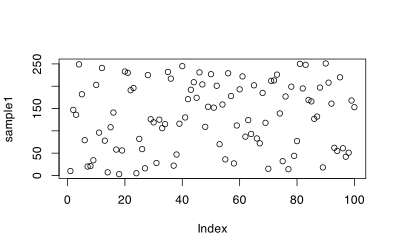
\includegraphics[keepaspectratio]{index_files/mediabag/lectures/L11-lcg_files/figure-pdf/lcg1-1.pdf}}

That looks like a pretty random collection of numbers to me.

Second, we stick with \(a = 13\) be the multiplier and \(x_1 = 10\) as
the seed, be decrease the increment by 1 to \(c = 16\).

\begin{Shaded}
\begin{Highlighting}[]
\NormalTok{sample2 }\OtherTok{\textless{}{-}} \FunctionTok{lcg}\NormalTok{(}\DecValTok{100}\NormalTok{, m, }\DecValTok{13}\NormalTok{, }\DecValTok{16}\NormalTok{, }\DecValTok{10}\NormalTok{)}
\FunctionTok{plot}\NormalTok{(sample2)}
\end{Highlighting}
\end{Shaded}

\pandocbounded{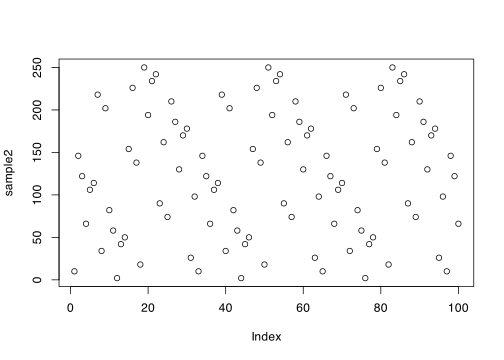
\includegraphics[keepaspectratio]{index_files/mediabag/lectures/L11-lcg_files/figure-pdf/lcg2-1.pdf}}

This doesn't seem as good. We can see there's some pattern where there
are parallel downward sloping lines. And also there seems to be some
sort of pattern \emph{within} these downward sloping lines, sometimes
with quite regularly-spaced points on those lines. And looking more
closely, we can see that actually the pattern of numbers repeats exactly
every 32 steps

\begin{Shaded}
\begin{Highlighting}[]
\FunctionTok{which}\NormalTok{(sample2 }\SpecialCharTok{==} \DecValTok{10}\NormalTok{)}
\end{Highlighting}
\end{Shaded}

\begin{verbatim}
[1]  1 33 65 97
\end{verbatim}

so we only ever see 32 of the possible 256 values. This doesn't seem to
look like a sequence of independent uniformly random points.

So again, it seems like LCG \emph{can} provide a good sequence of
pseudorandom numbers, but it seems quite sensitive to a good choice of
the parameters.

\end{example}

Is these examples, we've usually taken \(m\) to be a power of 2. There
are a few reasons for this:

\begin{itemize}
\item
  We will want to divide each term in the sequence \(x_i\) by \(m\) to
  get a number between \([0,1]\). If our number will be stored as a
  \(b\)-bit number, then it is makes sense to have created \(b\) bits
  (for an integer between \(0\) and \(m = 2^{b} - 1\)) in the first
  place. This means every integer in \(\{0, 1, \dots, m-1\}\)
  corresponds to exactly one \(b\)-bit number. Further this makes the
  division by \(m = 2^b\) extremely simple: you simple add ``0.'' (zero
  point\ldots) at the front of the number!
\item
  Modular arithmetic modulo a power of 2 is very simple for a computer.
  For a number in binary, the value modulo \(2^b\) is simply the last
  \(b\) bits of the number. So \texttt{10111001} modulo \(2^4\) is
  simply \texttt{1001}, the last four bits.
\item
  Having \(m = 2^b\) (or, more generally, having \(m\) being the product
  of lots of small prime factors) makes it easier to choose parameters
  such that the LCG is a good pseudorandom number generator \ldots{} as
  we shall see in the next section.
\end{itemize}

\section{Periods of LCGs}\label{periods-of-lcgs}

In an LCG, each number in the sequence depends only on the one before,
since \(x_{i+1} = (ax_i + c) \bmod m\). This means if we ever get a
single ``repeat'' in our sequence -- that is, if we see a number we have
seen at some point before -- then the whole sequence from that point on
will copy what came before.

For example, in the second part of Example~\ref{exm-lcg-easy}, the
sequence started \((1, 9, 1, \dots)\). As soon as we hit that repeat 1,
we know we're going to see that pattern \(1, 9\) repeated forever. We
say that this LCG has ``period'' 2. More generally, the \textbf{period}
of an LCG is the smallest \(k \geq 1\) such that \(x_{i+k} = x_i\) for
some \(i\).

We would like our LCGs to have a big period. If an LCG has a small
period, it will not look random, as we will just repeat the same small
number of values over and over again.

The smallest possible period is 1. That would be an extraordinarily bad
LCG, as it would just spit out the same number forever. The biggest
possible period is \(m\). That is because there are only \(m\) possible
values in \(\{0, 1, \dots, m-1\}\); so after \(m+1\) steps we must have
had a repeat, by the
\href{https://en.wikipedia.org/wiki/Pigeonhole_principle}{pigeonhole
principle}. Having the maximum period \(m\) is also called having ``full
period''.

Generally, the only way to find the period of an LCG is to run it for a
long time, and see how long it takes to start repeating. But,
conveniently, there \emph{is} a very easy way to tell if an LCG has the
maximum possible period \(m\), thanks to a result of TE Hull and AR
Dobell.

\begin{theorem}[Hull--Dobell
theorem]\protect\hypertarget{thm-hd}{}\label{thm-hd}

Consider the linear congruential generator
\(x_{i+1} = (ax_i + c) \bmod m\). This LCG has period \(m\) if and only
if the following three conditions hold:

\begin{enumerate}
\def\labelenumi{\arabic{enumi}.}
\item
  \(m\) and \(c\) are coprime;
\item
  \(a - 1\) is divisible by all prime factors of \(m\);
\item
  if \(m\) is divisible by 4, then \(a - 1\) is divisible by 4.
\end{enumerate}

\end{theorem}

If \(m = 2^b\) is a power of 2 (with \(b \geq 2\)), then the three
conditions simplify to a particularly pleasant form:

\begin{enumerate}
\def\labelenumi{\arabic{enumi}.}
\item
  \(c\) is odd;
\item
  \(a - 1\) is even;
\item
  \(a - 1\) is divisible by 4.
\end{enumerate}

Of course, the third point on the list implies the second. So we only
actually need to check \emph{two} things:

\begin{enumerate}
\def\labelenumi{\arabic{enumi}.}
\item
  \(c\) is odd
\item
  \(a\) is \(1 \bmod 4\) (that is, \(a\) is one more than a multiple of
  4).
\end{enumerate}

(We won't prove the Hull--Dobell theorem here -- it's some pretty tricky
number theory. But see
\href{https://leeds.primo.exlibrisgroup.com/permalink/44LEE_INST/1kmht9a/alma991012846439705181}{Knuth,
\emph{The Art of Computer Programming}}, \emph{Volume 2: Seminumerical
algorithms}, Subsubsection 3.2.1.2 if you really want a proof and have
sufficient number theory background.)

\begin{example}[]\protect\hypertarget{exm-periods}{}\label{exm-periods}

Let's go back to the earlier examples, and see if they have full periods
or not.

In the first LCG of Example~\ref{exm-lcg-easy}, we had \(m = 2^4\),
\(a = 5\) and \(c = 3\). Here, \(c\) is odd, and \(a = 4 + 1\) is
\(1 \bmod 4\). This LCG fulfils both conditions, so it has the maximum
possible period of 16.

In the second LCG of Example~\ref{exm-lcg-easy}, we had \(m = 2^4\),
\(a = 3\) and \(c = 6\). Here, \(c\) is even, and \(a\) is
\(2 \bmod 4\). This LCG does not fulfil both the conditions -- in fact,
it fails them both -- so it does not have the maximum possible period of
16. (We already saw that it in fact has period 2.)

In the first LCG of Example~\ref{exm-lcg-hard}, we had \(m = 2^8\),
\(a = 13\) and \(c = 17\). Here, \(c\) is odd, and \(a = 12 + 1\) is
\(1 \bmod 4\). This LCG fulfils both conditions, so it has the maximum
possible period of 256.

In the second LCG of Example~\ref{exm-lcg-hard}, we had \(m = 2^8\),
\(a = 13\) and \(c = 16\). Here, \(c\) is even, and \(a = 12 + 1\) is
\(1 \bmod 4\). So although this LCG does fulfil the second condition, it
does not fulfil the first, so it does not have the maximum possible
period of 256. (We already saw that it in fact has period 32.)

\end{example}

It normally a good idea to make sure your LCG has full period -- if it's
so easy to ensure, then why not? (That said, a very large but
not-quite-maximum period may be good enough. For example, if an LCG with
modulus \(2^{64}\) has a period of ``only'' \(2^{60}\), that might well
be enough: one million samples a second for one thousand years is only
\(2^{55}\) samples, so you'd never actually \emph{see} a repeat.)

But merely having full period (and a large modulus) isn't enough by
itself to guarantee an LCG will make a good pseudorandom number
generator. After all, the silly LCG \(x_{i+1} = x_i + 1\) has full
period, but the sequence
\[(0, 1, 2, 3, \dots, m-2, m-1, 0, 1, 2, \dots)\] will not look random.

\section{Statistical testing}\label{statistical-testing}

Before being used properly, any pseudorandom number generator is
subjected to a barrage of statistical tests, to check if its output
seems to ``look random''. Alongside checking it has a very large period,
the tester will want to check other statistical properties of
randomness. Even the best PRNGs might not pass every single such test.
See
\href{https://leeds.primo.exlibrisgroup.com/permalink/44LEE_INST/1fj430b/cdi_askewsholts_vlebooks_9781118728031}{Voss,
\emph{An Introduction to Statistical Computing}}, Subsection 1.1.2 for
more (non-examinable) material on statistical tests for randomness.

LCGs were considered state-of-the-art until the late-90s or so. However,
it was discovered that \(m\) needs be very big and the number of samples
used fairly small in order to pass some of the more stringent
statistical tests of randomness. For example, it's suggested that
\(n = 1\,000\,000\) (one million) samples from a full-period LCG with
modulus \(m = 2^{64}\) might be the limit before it starts ``not looking
random enough''. In particular, an LCG with a large period may not
actually see \emph{enough} repeats -- after all, random numbers will
have the occasional one-off repeat, just by chance. Compared to other
more modern methods (like R's default, the Mersenne Twister, mentioned
in the last lecture, discovered in 1997), an LCG requires quite a lot of
computation for only a modest number of samples. So while LCGs are still
admired for their simplicity and elegance, they have fallen out of
favour for cutting-edge computational work.

\textbf{Next time:} \emph{We'll use our pseudorandom uniform \([0,1]\)
random numbers to make random numbers with other discrete or uniform
distributions.}

\textbf{Summary:}

\begin{itemize}
\item
  Linear congruential generators are pseudorandom number generators
  based on the recurrence \(x_{n+1} = (ax_n + c) \bmod m\).
\item
  Any LCG will eventually repeat with periodic behaviour.
\item
  Suppose \(m\) is a power of 2. Then an LCG has full period \(m\) if
  and only if \(c\) is odd and \(a = 1 \bmod 4\).
\end{itemize}

You should now be able to answer all questions on
\hyperref[P2]{\textbf{Problem Sheet 2}}. Your answers will be discussed
in the problems class on \textbf{Thursday 31 October}.

\textbf{Read more:}
\href{https://leeds.primo.exlibrisgroup.com/permalink/44LEE_INST/1fj430b/cdi_askewsholts_vlebooks_9781118728031}{Voss,
\emph{An Introduction to Statistical Computing}}, Subsections 1.1.1 and
1.1.2.

\chapter*{Problem Sheet 2}\label{P2}
\addcontentsline{toc}{chapter}{Problem Sheet 2}

\markboth{Problem Sheet 2}{Problem Sheet 2}

\textbf{\hyperref[P2-sols]{Full solutions}} are now available.

This is Problem Sheet 2, which covers material from Lectures 7 to 11.
You should work through all the questions on this problem sheet in
advance of the problems class, which takes place in the lecture of
\textbf{Thursday 30 October}.

This problem sheet is to help you practice material from the module and
to help you check your learning. It is \emph{not} for formal assessment
and does not count towards your module mark.

If you want some brief informal feedback on \textbf{Question 1} (marked
★), you should submit your work electronically through Gradescope via
the module's Minerva page by \textbf{1400 on Tuesday 28 October}. (If
you hand-write solutions on paper, the easiest way to scan-and-submit
that work is using the Gradescope app on your phone.) I will return some
brief comments on your those two questions by the problems class on
Thursday 30 October. Because this informal feedback, and not part of the
official assessment, I cannot accept late work for any reason -- but I
am always happy to discuss any of your work on any question in my office
hours.

Full solutions will be released on Friday 31 October.

\chapter{Uniform and discrete}\label{uniform-and-discrete}

We've seen how to generate uniform random variates
\(U \sim \operatorname{U}[0,1]\), either using true physical randomness
or the output of a pseudorandom number generator. But in statistics --
whether performing Monte Carlo estimation or anything else -- we
typically want to sample from some other distribution \(X\).

In the next five lectures, we will look at ways we can transform the
uniform random variable \(U\) to take on different distributions
instead. We start today by looking at some important special cases.

\section{Uniform random variables}\label{uniform-random-variables}

We know how to generate \(U \sim \operatorname{U}[0,1]\). But suppose we
want to generate \(X \sim \operatorname{U}[a,b]\) instead, for some
\(a < b\); how can we do that.

Well, the original \(U\) has ``width'' 1, and we want \(X\) to have
width \(b - a\), so the first thing we should do is multiply by
\((b-a)\). This gives us \((b-a)U\), which we expect should be uniform
on \([0,b-a]\). Then we need to shift it, so it starts not a \(0\) but
at \(a\); we can do this by adding \(a\). This gives us \((b-a)U + a\),
which should be uniform on \([0 + a, (b-a) + a] = [a, b]\). So
\(X = (b-a)U + a\) would seem to give us the desired
\(X \sim \operatorname{U}[a,b]\) random variable.

We can check this seems to have worked by using a histogram, for
example.

\begin{example}[]\protect\hypertarget{exm-unif}{}\label{exm-unif}

Let \(U \sim \operatorname{U}[0,1]\). We can generate
\(X \sim \operatorname{U}[3,5]\) by \(X = 2U + 3\).

\begin{Shaded}
\begin{Highlighting}[]
\NormalTok{n }\OtherTok{\textless{}{-}} \FloatTok{1e5}
\NormalTok{Usamples }\OtherTok{\textless{}{-}} \FunctionTok{runif}\NormalTok{(n)}
\NormalTok{Xsamples }\OtherTok{\textless{}{-}} \DecValTok{2} \SpecialCharTok{*}\NormalTok{ Usamples }\SpecialCharTok{+} \DecValTok{3}
\FunctionTok{hist}\NormalTok{(Xsamples, }\AttributeTok{probability =} \ConstantTok{TRUE}\NormalTok{, }\AttributeTok{xlim =} \FunctionTok{c}\NormalTok{(}\DecValTok{2}\NormalTok{, }\DecValTok{6}\NormalTok{), }\AttributeTok{ylim =} \FunctionTok{c}\NormalTok{(}\DecValTok{0}\NormalTok{, }\FloatTok{0.6}\NormalTok{))}
\FunctionTok{curve}\NormalTok{(}\FunctionTok{dunif}\NormalTok{(x, }\DecValTok{3}\NormalTok{, }\DecValTok{5}\NormalTok{), }\AttributeTok{add =} \ConstantTok{TRUE}\NormalTok{, }\AttributeTok{n =} \DecValTok{1001}\NormalTok{, }\AttributeTok{lwd =} \DecValTok{2}\NormalTok{, }\AttributeTok{col =} \StringTok{"blue"}\NormalTok{)}
\end{Highlighting}
\end{Shaded}

\pandocbounded{\includegraphics[keepaspectratio]{index_files/mediabag/lectures/L12-uniform-discrete_files/figure-pdf/unnamed-chunk-1-1.pdf}}

Here, we used the \texttt{probability\ =\ TRUE} argument to the
histogram function \texttt{hist()} to plot the density on the
\(y\)-axis, rather than the raw number of samples. The density should
match the probability density function of the random variable \(X\). We
drew the PDF of \(X\) over the histogram in blue, and can see it is a
superb match.

\end{example}

But what if we very formally wanted to \emph{prove} that
\(X = (b-a)U + a\) definitely has the distribution
\(X \sim \operatorname{U}[a,b]\); how could we do that?

The best way to give a formal proof of something like this is to use the
\textbf{cumulative distribution function} (CDF). Recall that the CDF
\(F_Y\) of a distribution \(Y\) is the function
\(F_Y(y) = \mathbb P(Y \leq y)\). One benefit of the CDF is it works
equally well for both discrete and continuous random variables, so we
don't need to give separate arguments for discrete and continuous cases.

The CDF of the standard uniform distribution
\(U \sim \operatorname{U}[0,1]\) is
\begin{equation}\phantomsection\label{eq-cdf-u}{ F_U(u) = \begin{cases} 0 & u < 0 \\ u & 0 \leq u \leq 1 \\ 1 & u > 1 , \end{cases} }\end{equation}
and the CDF of any uniform distribution \(X \sim \operatorname{U}[a,b]\)
is
\begin{equation}\phantomsection\label{eq-cdf-x}{ F_X(x) = \begin{cases} 0 & x < a \\ \displaystyle\frac{x - a}{b-a} & a \leq x \leq b \\ 1 & x > b . \end{cases} }\end{equation}
So to show that \(X = (b-a)U + a \sim \operatorname{U}[a,b]\), we take
the fact that \(U\) has the CDF in Equation~\ref{eq-cdf-u} and try to
use it to show that \(X\) has the CDF in Equation~\ref{eq-cdf-x}.

Indeed, we have
\[ F_X(x) = \mathbb P(X \leq x) = \mathbb P\big((b-a)U + a \leq x\big) = \mathbb P \left( U \leq \frac{x - a}{b-a}\right) . \]
But putting \(u = (x - a)/(b - a)\) in Equation~\ref{eq-cdf-u}, does
indeed give the CDF in Equation~\ref{eq-cdf-x}. The lower boundary
\(u < 0\) becomes \(x < 0 \times (b-a) + a = a\); the upper boundary
\(u > b\) becomes \(x > 1 \times(b-a) + a = b\); and, in between, the
CDF \(u\) becomes \((x - a)/(b - a)\). Thus we have proven that \(X\)
has the CDF of the \(\operatorname{U}[a,b]\) distribution, as required.

\section{Discrete random variables}\label{discrete-random-variables}

Suppose we want to simulate a Bernoulli trial; that is, a random
variable \(X\) that is 1 with probability \(p\) and 0 with probability
\(1 - p\), for some \(p\) with \(0 < p < 1\). As ever, we only have a
standard uniform \(U \sim \operatorname{U}[0,1]\) to work with. How can
we form our Bernoulli trial?

Here are two possible ways:

\begin{itemize}
\item
  If \(U < p\), then take \(X = 1\); while if \(U \geq p\), take
  \(X = 0\). Note that \(\mathbb P(X = 1) = \mathbb P(U < p) = p\) and
  \(\mathbb P(X = 0) = \mathbb P(U \geq p) = 1 - \mathbb P(U < p) = 1 - p\),
  as required.
\item
  Alternatively: if \(U \leq 1 -p\), take \(X' = 0\); while if
  \(U > p\), take \(X' = 1\).
\end{itemize}

The first method is just the second method with \(U\) replaced by
\(1 - U\). Interestingly, that means we can generate two different
Bernoulli trials \(X\) and \(X'\) from the same \(U\), which will
therefore be negatively correlated. Although there's unlikely to be any
situation where a Bernoulli trial would be used in Monte Carlo
estimation, in theory, the two versions \((X, X')\) generated from the
same \(U\) could potentially be used as antithetic variables.

What about more general discrete random variables? Suppose a random
variable takes values \(x_1, x_2, \dots\) with probabilities
\(p_1, p_2, \dots\). We can think of these probabilities as splitting up
the interval \([0,1]\) into subintervals of lengths \(p_1, p_2, \dots\),
since these probabilities add up to 1.

\begin{center}
\pandocbounded{
\includegraphics[keepaspectratio]{index_files/mediabag/lectures/L12-numberline-1.pdf}}
\end{center}

So the first interval is \(I_1 = (0, p_1]\); the second interval is
\((p_1, p_1 + p_2]\); the third intervals is
\((p_1 + p_2, p_1 + p_2 + p_3]\), and so on. We then pick a point \(U\)
from \([0,1]\) uniformly at random, and whichever interval \(I_i\) it is
in, take the corresponding value \(x_i\).

In terms of the CDF, we have \(F_X(x_i) = p_1 + p_2 + \cdots + p_i\), so
the intervals are of the form \((F_X(x_{i-1}), F_X(x_i)]\). So we can
think of this as rounding \(F_X(U)\) up to the next \(F_X(x_i)\), then
taking that value \(x_i\).

\begin{example}[]\protect\hypertarget{exm-binom}{}\label{exm-binom}

Consider generating a binomial distribution
\(X \sim \operatorname{Bin}(5, \frac12)\). The PMF and CDF are as shown
below

\begin{longtable}[]{@{}
  >{\centering\arraybackslash}p{(\linewidth - 10\tabcolsep) * \real{0.3333}}
  >{\centering\arraybackslash}p{(\linewidth - 10\tabcolsep) * \real{0.1333}}
  >{\centering\arraybackslash}p{(\linewidth - 10\tabcolsep) * \real{0.1333}}
  >{\centering\arraybackslash}p{(\linewidth - 10\tabcolsep) * \real{0.1333}}
  >{\centering\arraybackslash}p{(\linewidth - 10\tabcolsep) * \real{0.1333}}
  >{\centering\arraybackslash}p{(\linewidth - 10\tabcolsep) * \real{0.1333}}@{}}
\toprule\noalign{}
\begin{minipage}[b]{\linewidth}\centering
\textbf{value} \(x\)
\end{minipage} & \begin{minipage}[b]{\linewidth}\centering
\(0\)
\end{minipage} & \begin{minipage}[b]{\linewidth}\centering
\(1\)
\end{minipage} & \begin{minipage}[b]{\linewidth}\centering
\(2\)
\end{minipage} & \begin{minipage}[b]{\linewidth}\centering
\(3\)
\end{minipage} & \begin{minipage}[b]{\linewidth}\centering
\(4\)
\end{minipage} \\
\midrule\noalign{}
\endhead
\bottomrule\noalign{}
\endlastfoot
\textbf{PMF} \(p(x)\) & \(\frac{1}{32}\) & \(\frac{5}{32}\) &
\(\frac{10}{32}\) & \(\frac{10}{32}\) & \(\frac{5}{32}\) \\
\textbf{CDF} \(F_X(x)\) (fraction) & \(\frac{1}{32}\) & \(\frac{6}{32}\)
& \(\frac{16}{32}\) & \(\frac{26}{32}\) & \(\frac{31}{32}\) \\
\textbf{CDF} \(F_X(x)\) (decimal) & 0.03125 & 0.1875 & 0.5 & 0.8125 &
0.96875 \\
\end{longtable}

~

Suppose I want a sample from this, based on the uniform variate
\(u_1 = 0.7980\). We see that \(u_1\) is bigger that \(F_X(2) = 0.5\)
(the upper end of the ``2'' interval) but less than \(F_X(3) = 0.8125\)
(the upper end of the ``3'' interval), so falls into the ``3'' interval.
So our first binomial variate is \(x_1 = 3\).

If we then got the next uniform variate \(u_2 = 0.4353\), we would see
that \(u_2\) is between \(F_X(1) = 0.1875\) and \(F_X(2) = 0.5\), so
would take \(x_2 = 2\) for our next binomial variate.

\end{example}

\textbf{Next time:} \emph{Sampling from continuous distribution using
the CDF.}

\textbf{Summary:}

\begin{itemize}
\item
  If \(U \sim \operatorname{U}[0,1]\), then
  \(X = (b-a)U + a \sim \operatorname{U}[a,b]\).
\item
  A discrete random variable can be generated by splitting \([0,1]\)
  into subintervals with lengths according to the probabilities, then
  picking a point from the interval at random.
\end{itemize}

Remember that your answers to \hyperref[P2]{\textbf{Problem Sheet 2}}
will be discussed in the problems class on \textbf{Thursday 31 October}.

\textbf{Read more:}
\href{https://leeds.primo.exlibrisgroup.com/permalink/44LEE_INST/1fj430b/cdi_askewsholts_vlebooks_9781118728031}{Voss,
\emph{An Introduction to Statistical Computing}}, Sections 1.2 and 1.3.

\chapter{Inverse transform method}\label{inverse-transform-method}

\[ \]

\section{Inverse CDF}\label{inverse-cdf}

We have started looking at how to transform a standard uniform random
variable \(U \sim \operatorname{U}[0,1]\) into any other distribution
\(X\).

Last lecture, we saw how to do this for other uniform distributions and
for discrete random variables. Booth involved the cumulative
distribution function \(F(x) = \mathbb P(X \leq x)\). For generating a
wider class of random variables (including continuous random variables)
the CDF will continue to be important. In fact, it is the \emph{inverse}
of the CDF that will play a crucial role.

It seems natural to define the inverse \(F^{-1}\) of the CDF in just the
same way we would define the inverse of any other function: that
\(F^{-1}(u)\) is the unique value \(x\) such that \(F(x) = u\). This is
illustrated in the figure below.

{[}picture{]}

This definition works fine for a purely continuous distribution that
doesn't have any ``gaps'' in the set of values it can take. But for a
general random variable, there are two problems with this definition.

\begin{enumerate}
\def\labelenumi{\arabic{enumi}.}
\item
  If \(X\) has any point masses -- points \(x\) with strictly positive
  probability \(\mathbb P(X = x) > 0\) of hitting that point exactly --
  then \(F\) may ``jump past'' the value \(u\), so there is \emph{no}
  value \(x\) such that \(F(u)\). (See the blue line on the graph
  below.)
\item
  If there is an interval on the line where \(X\) has probability zero,
  then all the \(x\)s in that interval have the same value of
  \(F(x) = u\), so there is no \emph{unique} value \(x\) such that
  \(F(x) = u\). (See the red line on the graph below.)
\end{enumerate}

{[}picture{]}

It turns out that the best way to solve this is the following. For the
first obstacle, if there are many points \(x\) with \(F(x) = u\), we
take the first one -- that is, the smallest \(x\) with \(F(x) = u\). For
the second obstacle, we take the value of the smallest \(x\) where
\(F(x)\) is above \(u\), which comes right at the jump. These two cases
are illustrated below.

{[}picture{]}

These two awkward cases can be encapsulated in the following definition.

\begin{definition}[]\protect\hypertarget{def-cdf-inv}{}\label{def-cdf-inv}

Let \(X\) be a random variable with cumulative distribution function
\(F_X(x) = \mathbb P(X \leq x)\). Then the \textbf{inverse cumulative
distribution function} (inverse CDF) \(F_X^{-1}\) is defined for
\(u \in (0,1)\) by
\[ F^{-1}_X(u) = \min \big \{x : F_X(x) \geq u \big\} . \]

\end{definition}

You should check that you agree this definition matches the discussion
above.

\section{Inverse transform}\label{inverse-transform}

The inverse transform method works like this: To generate \(X\), simply
apply the inverse CDF \(F^{-1}\) to a standard uniform random variable
\(U\).

\begin{theorem}[]\protect\hypertarget{thm-inv-trans}{}\label{thm-inv-trans}

Let \(F\) be a cumulative distribution function, and let \(F^{-1}\) be
its inverse. Let \(U \sim \operatorname{U}[0,1]\). Then
\(X = F^{-1}(U)\) has cumulative distribution function \(F\).

\end{theorem}

\begin{proof}
We need to show that \(\mathbb P(X \leq x) = F(x)\) when this is in
\((0,1)\). The proof is very easy if \(F\) has no ``gaps'' or ``jumps''
as described above. Then, we simply have
\[ \mathbb P(X \leq x) = \mathbb P\big(F^{-1}(U) \leq x\big) = \mathbb P\big(U \leq F(x)\big) = F(x), \]
where we have simply ``undone'' the function \(F^{-1}\) and used that
\(\mathbb P(U \leq u) = u\) for \(u \in (0,1)\).

For the general case, we need to be just a little bit more careful. We
have
\[ \mathbb P(X \leq x) = \mathbb P\big(F^{-1}(U) \leq x\big) = \mathbb P\big(\min\{y : F(y) \geq U \} \leq x \big) .\]
If \(x\) is bigger than the minimum \(y\) with \(F(y) \geq u\), then
certainly \(F(x) \geq u\) as well; while if \(F(x) \geq u\), then \(x\)
must be at least as big as the minimum \(y\) for which \(F(y) \geq u\).
Hence \(\min\{y : F(y) \geq U \} \leq x\) if and only if
\(F(x) \geq U\). So
\[ \mathbb P(X \leq x) = \mathbb P\big(\min\{y : F(y) \geq U \} \leq x \big) = \mathbb P\big(F(x) \geq U\big) = \mathbb P(U \leq F(x)\big) = F(x), \]
as before.
\end{proof}

The method -- known as the \textbf{inverse transform method} gives a
simple way to generate any random variable \(X\) for which the inverse
CDF \(F_X^{-1}\) can be computed easily.

This is not all random variables, however. In particular, the inverse
CDF of the normal distribution does not have a closed form, so this does
not give a way of sampling normal distributions. Later we'll see other
methods that allow us to sample from normal random variables.

\section{Examples}\label{examples-2}

Let's see some examples. The idea for all these problems is ``Write
\(U = F(X)\), then invert, to get \(X = F^{-1}(U)\).''

\begin{example}[]\protect\hypertarget{exm-exp}{}\label{exm-exp}

Let \(X \sim \operatorname{Exp}(\lambda)\) be an exponential
distribution with rate \(\lambda\). This has PDF
\(f(x) = \lambda \ee^{-\lambda x}\) for \(x \geq 0\) and CDF
\(F(x) = 1 - \ee^{-\lambda x}\).

We write \(U = F(X)\) and invert it to make \(X\) the subject. So
\(U = 1 - \ee^{-\lambda X}\), and therefore
\[ X = -\frac{1}{\lambda} \log(1 - U) . \]

We should check that this really does have an exponential distribution.

\begin{Shaded}
\begin{Highlighting}[]
\NormalTok{rate }\OtherTok{\textless{}{-}} \FloatTok{0.5}
\NormalTok{n }\OtherTok{\textless{}{-}} \FloatTok{1e5}
\NormalTok{unif }\OtherTok{\textless{}{-}} \FunctionTok{runif}\NormalTok{(n)}
\NormalTok{samples }\OtherTok{\textless{}{-}} \SpecialCharTok{{-}}\NormalTok{(}\DecValTok{1} \SpecialCharTok{/}\NormalTok{ rate) }\SpecialCharTok{*} \FunctionTok{log}\NormalTok{(}\DecValTok{1} \SpecialCharTok{{-}}\NormalTok{ unif)}

\FunctionTok{hist}\NormalTok{(samples, }\AttributeTok{probability =} \ConstantTok{TRUE}\NormalTok{)}
\FunctionTok{curve}\NormalTok{(}\FunctionTok{dexp}\NormalTok{(x, rate), }\AttributeTok{add =} \ConstantTok{TRUE}\NormalTok{, }\AttributeTok{col =} \StringTok{"blue"}\NormalTok{, }\AttributeTok{lwd =} \DecValTok{2}\NormalTok{)}
\end{Highlighting}
\end{Shaded}

\pandocbounded{\includegraphics[keepaspectratio]{index_files/mediabag/lectures/L13-inverse_files/figure-pdf/unnamed-chunk-1-1.pdf}}

Looks like an accurate sample!

Since \(1 - U\) has the same distribution as \(U\), it can be more
convenient to simply write \[ X' = -\frac{1}{\lambda} \log U \] instead.

Alternatively, since \(X\) and \(X'\) are not independent and both have
the same exponential distribution, they are a candidate to use as an
antithetic pair in Monte Carlo estimation.

\end{example}

\begin{example}[]\protect\hypertarget{exm-rayleigh}{}\label{exm-rayleigh}

Consider \(X\) with PDF
\[ f(x) = \frac{x}{\gamma} \,\exp \left(-\frac{x^2}{2\gamma}\right)\]
for \(x \geq 0\), and CDF
\[ F(x) = 1 - \exp\left(-\frac{x^2}{2\gamma}\right) \] This is known as
the \textbf{Rayleigh distribution} with scale parameter \(\gamma\).

Again, we write \(U = F(X)\) and invert. so
\[ U = 1 - \exp\left(-\frac{X^2}{2\gamma}\right)  \] so
\[ X = \sqrt{-2\gamma\log(1-U)} . \]

Again, \(X' = \sqrt{-2\gamma\log U}\) is a slightly simpler expression,
or could be used in an antithetic variables Monte Carlo approach.

\end{example}

\begin{example}[]\protect\hypertarget{exm-unif}{}\label{exm-unif}

Suppose \(X \sim \operatorname{U}[a,b]\), then
\[ F(x) = \frac{x-a}{b-a} \] (except for when \(F(x) = 0\) or \(1\)).

Write \(U = F(X)\) and invert. We get \(X = (b-a)U + a\). This is
precisely the method for generating general uniform distributions that
we saw in the last lecture.

\end{example}

\begin{example}[]\protect\hypertarget{exm-discrete}{}\label{exm-discrete}

Let \(X\) be discrete on the values \(x_1, x_2, \dots\) with
probabilities \(p_1, p_2, \dots\). The CDF is
\[ F(x) = \begin{cases} 0 & x < x_1 \\
p_1 & x_1 \leq x < x_2 \\
p_1 + p_2 & x_2 \leq x < x_3 \\
p_1 + p_2 + p_3 & x_3 \leq x < x_4 \\
\cdots & \cdots . \end{cases} \]

Remembering the rule for ``jumps'' in the CDF, we see that the inverse
CDF is \[ F^{-1}(u) = \begin{cases} x_1 & u < p_1 \\
x_2 & p_1 \leq x < p_1 + p_2 \\
x_3 & p_1 + p_2 \leq x < p_1 + p_2 + p_3 \\
\cdots & \cdots . \end{cases} \] Taking \(X = F^{-1}(U)\) gives the same
method for generating discrete random variables as we discussed in the
last lecture.

\end{example}

\begin{example}[]\protect\hypertarget{exm-pdf-gen}{}\label{exm-pdf-gen}

\emph{Consider a distribution with PDF}
\[ f(x) = \begin{cases} x^2 & 0 \leq x \leq 1 \\
\frac{2}{3} & 1 < x \leq 2 \\
0 & \text{otherwise.} \end{cases} \] \emph{Show how to sample \(X\)
using a standard uniform random variable \(U\).}

This is a standard sort of question. First we have to find the CDF, then
we have to invert it.

We find the CDF from the PDF by integrating. For \(0 \leq x \leq 1\), we
have
\[ F(x) = \int_0^x f(y) \, \mathrm{d}y = \int_0^x y^2 \,\mathrm{d}y = \tfrac13 x^3. \]
Then for \(1 < x \leq 2\), we have
\[ F(x) = F(1) + \int_1^x f(y) \, \mathrm{d}y = \tfrac13 + \int_1^x \tfrac23 \,\mathrm{d}y = \tfrac13 + \tfrac23 x - \tfrac23 = \tfrac23 x - \tfrac13 . \]

For \(0 \leq U < \leq F(1) = \tfrac13\), we have \(U = \tfrac13 X^3\),
so \(X = \sqrt[3]{3U}\). For \(F(1) = \tfrac13 < U \leq 1\), we have
\(U = \tfrac23 X - \tfrac13\), so \(X = \tfrac32 U + \tfrac12\). So the
inverse transform is
\[ X = \begin{cases} \sqrt[3]{3U} & U \leq \frac13 \\ \tfrac32 U + \tfrac12 & U > \tfrac13 . \end{cases} \]

\end{example}

\section{Box--Muller transform}\label{boxmuller-transform}

\emph{{[}This was actually lectured at the beginning of Lecture 14, but
belongs in this section.{]}}

While the inverse transform method is very powerful, we have mentioned
that it doesn't work directly for the normal distribution, which does
not have an exact closed form for the inverse CDF. (Although R does
actually use the inverse transform method in its \texttt{rnorm()}
function by using an \emph{approximation} to the inverse CDF.)

Instead, the \textbf{Box--Muller transform} (discovered by the
statistician GEP Box and the computer scientist Marvin E Muller in 1958)
is a clever way to easily transform a standard uniform into a normal
distribution.

Actually, that's not quite true. Rather than transforming one standard
uniform \(U\) into one normal distribution \(X\), it instead transforms
\emph{two} independent standard uniforms \(U, V\) into \emph{two} normal
distributions \(X, Y\). (There is some profound mathematical sense in
which the two-dimensional bivariate normal is somehow a more ``deeply''
important mathematical object than the one-dimensional univariate normal
we are used to, but we don't have time to get into that here.)

First, let's note it suffices to produce a standard normal
\(X \sim \operatorname{N}(0,1)\). Any other normal distribution
\(W \sim \operatorname{N}(\mu, \sigma^2)\) can then be formed as
\(W = \sigma X + \mu\).

The idea of the Box--Muller transform is based on converting the two
standard normal distributions \((X, Y)\) from cartesian coordinates into
polar coordinates \((R, \Theta)\). (Those of you who have know
\href{https://mpaldridge.github.io/math1710/L16-normal.html\#normal-properties}{how
to calculate the Gaussian integral} will have seen this idea before.)

{[}picture{]}

\begin{theorem}[]\protect\hypertarget{thm-box-muller-1}{}\label{thm-box-muller-1}

Let \(X, Y \sim \operatorname{N}(0,1)\) be independent standard normal
distributions. Write
\[ R = \sqrt{X^2 + Y^2} \qquad\qquad \Theta = \tan \frac{Y}{X} \] for
the radius and the angle of \((X, Y)\) in polar coordinates. Then the
radius \(R\) has a Rayleigh distribution with scalar parameter
\(\gamma = 1\), the angle \(\Theta\) has a uniform distribution on
\([0, 2\pi]\), and \(R\) and \(\Theta\) are independent.

\end{theorem}

\begin{proof}
The joint PDF of \((X,Y)\) is \begin{align}
f_{X,Y}(x, y) \,\mathrm{d}x\,\mathrm{d}y &= f_X(x) \,f_Y(y) \,\mathrm{d}x\,\mathrm{d}y \\
&= \frac{1}{\sqrt{2\pi}}\, \exp \big(-\tfrac12 x^2\big) \, \frac{1}{\sqrt{2\pi}} \,\exp \big(-\tfrac12 y^2\big) \,\mathrm{d}x\,\mathrm{d}y \\
&= \frac{1}{2\pi} \,\exp \big(-\tfrac12 (x^2 + y^2)\big) \,\mathrm{d}x\,\mathrm{d}y .  
\end{align} \{\#eq-box-1\} The joint PDF of \((R, \Theta)\) is
\begin{align}
f_{R, \Theta}(r, \theta) \,\mathrm{d}r\,\mathrm{d}\theta &= f_R(r) \,f_\Theta(\theta) \,\mathrm{d}r\,\mathrm{d}\theta \\
&= r\exp \big(-\tfrac12 r^2\big) \, \frac{1}{2\pi}\, \mathrm{d}r\,\mathrm{d}\theta , 
\end{align} \{\#eq-box-2\}

But in \textbf{?@eq-box-1}, we can substitute \(r = x^2 + y^2\) and
\(\mathrm{d}x\,\mathrm{d}y = r\,\mathrm{d}r\,\mathrm{d}\theta\), and get
\textbf{?@eq-box-2}.
\end{proof}

So we've reduced the problem of sample two normal distributions to
sampling a Rayleigh (with scale parameter 1) and a uniform (on
\([0, 2\pi]\)). But we know how to do this. We saw in
Example~\ref{exm-rayleigh} that we can take \(R = \sqrt{-2 \log U}\) (or
\(\sqrt{-2 \log(1-U)}\)), and we saw in the last lecture that we can
take \(\Theta = 2\pi V\). We can then transform back into cartesian
coordinates with \begin{align}
X &= R\cos \Theta =  \sqrt{-2 \log U} \cos(2\pi V) \\
Y &= R\sin \Theta =  \sqrt{-2 \log U} \sin(2\pi V) .
\end{align}

\begin{Shaded}
\begin{Highlighting}[]
\NormalTok{n }\OtherTok{\textless{}{-}} \FloatTok{1e5}
\NormalTok{unif1 }\OtherTok{\textless{}{-}} \FunctionTok{runif}\NormalTok{(n)}
\NormalTok{unif2 }\OtherTok{\textless{}{-}} \FunctionTok{runif}\NormalTok{(n)}
\NormalTok{rad }\OtherTok{\textless{}{-}} \FunctionTok{sqrt}\NormalTok{(}\SpecialCharTok{{-}}\DecValTok{2} \SpecialCharTok{*} \FunctionTok{log}\NormalTok{(unif1))}
\NormalTok{ang }\OtherTok{\textless{}{-}} \DecValTok{2} \SpecialCharTok{*}\NormalTok{ pi }\SpecialCharTok{*}\NormalTok{ unif2}
\NormalTok{samples }\OtherTok{\textless{}{-}} \FunctionTok{c}\NormalTok{(rad }\SpecialCharTok{*} \FunctionTok{cos}\NormalTok{(ang), rad }\SpecialCharTok{*} \FunctionTok{sin}\NormalTok{(ang))}

\FunctionTok{hist}\NormalTok{(samples, }\AttributeTok{probability =} \ConstantTok{TRUE}\NormalTok{, }\AttributeTok{breaks =} \DecValTok{50}\NormalTok{, }\AttributeTok{xlim =} \FunctionTok{c}\NormalTok{(}\SpecialCharTok{{-}}\DecValTok{4}\NormalTok{, }\DecValTok{4}\NormalTok{))}
\FunctionTok{curve}\NormalTok{(}\FunctionTok{dnorm}\NormalTok{(x), }\AttributeTok{add =} \ConstantTok{TRUE}\NormalTok{, }\AttributeTok{col =} \StringTok{"blue"}\NormalTok{, }\AttributeTok{lwd =} \DecValTok{2}\NormalTok{)}
\end{Highlighting}
\end{Shaded}

\pandocbounded{\includegraphics[keepaspectratio]{index_files/mediabag/lectures/L13-inverse_files/figure-pdf/unnamed-chunk-2-1.pdf}}

This confirms that we get an excellent match to the normal distribution.

\textbf{Next time:} \emph{Sampling using rejection.}

\textbf{Summary:}

\begin{itemize}
\item
  The inverse \(F^{-1}\) of a CDF \(F\) is defined by
  \(F^{-1}_X(u) = \min \big \{x : F_X(x) \geq u \big\}\).
\item
  The inverse transform method converts \(U \sim \operatorname{U}[0,1]\)
  to a random variable with CDF by setting \(X = F^{-1}(U)\). That is:
  Set \(U = F(X)\), and rearrange to make \(X\) the subject.
\item
  The Box--Muller transform is a way to generate two independent
  standard normal distributions. Set \(R\) to Rayleigh with scale
  parameter 1, set \(\Theta \sim \operatorname{U}[0,2\pi]\), then take
  \(X = R \cos \Theta\) and \(Y = R \sin \Theta\).
\end{itemize}

\textbf{Read more:}
\href{https://leeds.primo.exlibrisgroup.com/permalink/44LEE_INST/1fj430b/cdi_askewsholts_vlebooks_9781118728031}{Voss,
\emph{An Introduction to Statistical Computing}}, Section 1.3.

\chapter{Rejection sampling}\label{rejection-sampling}

\[ \]

\section{Rejection}\label{rejection}

In the last two lectures, we have taken standard uniform
\(U \sim \operatorname{U}[0,1]\) random variables, and have applied a
function to them to transform into some other distribution \(X\). One
\(U\) gets turned into one \(X\). (Or, for the Box--Muller transform,
two \(U\)s become two \(X\)s.)

But so far, we have taken each sample we are given. But another way to
get a different distribution is to throw out samples we don't like and
wait until we get a sample we do like. This is called \textbf{rejection
sampling}.

Suppose we want not a \(\operatorname{U}[0,1]\) random variable but
instead a \(\operatorname{U}[0,\tfrac12]\) random variable. One way
we've already seen to do this is by the inverse transform method: simply
multiply \(U\) by \(\tfrac12\). But we could also do this by rejection.
We start with a proposed sample \(U \sim \operatorname{U}[0,1]\). If
\(U \leq \tfrac12\), we ``accept'' the sample, and keep it. But if
\(U > \tfrac12\), we ``reject'' the samples -- we throw it away and ask
for a new one. We keep proposing samples until we accept one that's less
than \(\tfrac12\). It should be easy to convince yourself that we get a
\(\operatorname{U}[0,\tfrac12]\) random variable this way. (But we'll
prove it later, if not.)

The advantage of rejection sampling is that it can help us get samples
from some distributions that we couldn't access with the inverse
transform method. The disadvantage is that it can be costly or slow,
because we may have to reject lots of samples before finding enough that
we can accept. The more often we reject samples, the slower the
procedure will be.

Rejection sampling is particularly useful for sampling from a
conditional distribution, such as the conditional distribution of \(Y\)
given that \(Y \in A\): we simply accept a sample \(y\) if \(y \in A\)
and reject it if not.

\begin{example}[]\protect\hypertarget{exm-cond}{}\label{exm-cond}

Let \(Y \sim \operatorname{N}(0, 1)\). Suppose we wish to use Monte
Carlo estimation to estimate \(\mathbb E(Y \mid Y \geq 1)\).

To do this, we will need samples from the conditional distribution
\(Y \mid Y \geq 1\). So we accept proposed standard normal samples that
are at least 1, and reject proposed samples that are less than 1.

There are two ways we could run this in practice. First, we could decide
to take \(n\) proposal samples from \(Y\) and just see how many get
accepted.

\begin{Shaded}
\begin{Highlighting}[]
\NormalTok{n\_prop }\OtherTok{\textless{}{-}} \FloatTok{1e6}
\NormalTok{props   }\OtherTok{\textless{}{-}} \FunctionTok{rnorm}\NormalTok{(n\_prop)}
\NormalTok{accepts }\OtherTok{\textless{}{-}}\NormalTok{ props[props }\SpecialCharTok{\textgreater{}=} \DecValTok{1}\NormalTok{]}
\FunctionTok{length}\NormalTok{(accepts)}
\end{Highlighting}
\end{Shaded}

\begin{verbatim}
[1] 158933
\end{verbatim}

\begin{Shaded}
\begin{Highlighting}[]
\NormalTok{MCest1 }\OtherTok{\textless{}{-}} \FunctionTok{mean}\NormalTok{(accepts)}
\NormalTok{MCest1}
\end{Highlighting}
\end{Shaded}

\begin{verbatim}
[1] 1.526205
\end{verbatim}

We end up accepting around 160,000 samples out of the 1,000,000
proposals we had to start with.

Second, we could keep proposing as many samples as needed until we reach
some desired number of acceptances.

\begin{Shaded}
\begin{Highlighting}[]
\NormalTok{n\_acc }\OtherTok{\textless{}{-}} \FloatTok{1e5}

\NormalTok{samples }\OtherTok{\textless{}{-}} \FunctionTok{rep}\NormalTok{(}\DecValTok{0}\NormalTok{, n\_acc)}
\NormalTok{count }\OtherTok{\textless{}{-}} \DecValTok{0}
\ControlFlowTok{for}\NormalTok{ (i }\ControlFlowTok{in} \DecValTok{1}\SpecialCharTok{:}\NormalTok{n\_acc) \{}
\NormalTok{  newsample }\OtherTok{\textless{}{-}} \DecValTok{0}
  \ControlFlowTok{while}\NormalTok{ (newsample }\SpecialCharTok{\textless{}} \DecValTok{1}\NormalTok{) \{}
\NormalTok{    newsample }\OtherTok{\textless{}{-}} \FunctionTok{rnorm}\NormalTok{(}\DecValTok{1}\NormalTok{)}
\NormalTok{    count }\OtherTok{\textless{}{-}}\NormalTok{ count }\SpecialCharTok{+} \DecValTok{1}
\NormalTok{  \}}
\NormalTok{  samples[i] }\OtherTok{\textless{}{-}}\NormalTok{ newsample}
\NormalTok{\}}
\NormalTok{count}
\end{Highlighting}
\end{Shaded}

\begin{verbatim}
[1] 632946
\end{verbatim}

\begin{Shaded}
\begin{Highlighting}[]
\NormalTok{MCest2 }\OtherTok{\textless{}{-}} \FunctionTok{mean}\NormalTok{(samples)}
\NormalTok{MCest2}
\end{Highlighting}
\end{Shaded}

\begin{verbatim}
[1] 1.526
\end{verbatim}

This required taking about 630,000 proposals to get 100,000 acceptances.

Here we used a ``\texttt{while}'' loop to keep taking samples
\emph{until} we go one that was not less than 1. The lines involving
\texttt{count} were just so I could see how many proposals ended up
being needed -- these aren't an integral part of the code.

\end{example}

\section{Acceptance probability}\label{acceptance-probability}

So far, we have looked at always accepting or always rejecting a
proposed sample, depending on its value. But we could ``perhaps'' accept
some proposals too. Suppose we are already sampling from some
distribution \(Y\) (perhaps generated via the inverse transform method,
for example). If we see the proposed sample \(Y = x\), we could accept
it with some \textbf{acceptance probability} \(\alpha(x) \in [0,1]\). We
can control the accepted samples more delicately by adjusting this
acceptance function \(\alpha\) to values that aren't just 0 or 1.

What is the distribution of an accepted sample \(X\)?

Well, using Bayes' theorem, we have in the discrete case
\[\mathbb P(X = x) = \mathbb P(Y = x \mid \text{accept}) = \frac{\mathbb P(Y = x)\,\mathbb P(\text{accept} \mid Y = x)}{\mathbb P(\text{accept})} = \frac{1}{Z} \alpha(x)\,\mathbb P(Y = x) .\]
where \(Z = \mathbb P(\text{accept})\) is the normalising constant. In
the continuous case, with \(g\) the PDF of the original \(Y\) and \(f\)
the PDF of the accepted \(X\), we have
\[ f(x) = g(x \mid \text{accept}) = \frac{g(x)\,\mathbb P(\text{accept} \mid X = x)}{\mathbb P(\text{accept})} = \frac{1}{Z}\,\alpha(x)\,g(x) , \]
where \(Z = \mathbb P(\text{accept})\) again.

\begin{example}[]\protect\hypertarget{exm-normcos}{}\label{exm-normcos}

Suppose we wish to sample from the distribution
\begin{equation}\phantomsection\label{eq-distprop}{ f(x) \propto \exp\big(-\tfrac12x^2\big)\,(\sin^2 x) .}\end{equation}
How can we do this?

Well, we can note that the PDF of the standard normal is
\[ g(x) = \frac{1}{2\pi}\,\exp\big(-\tfrac12x^2\big) \propto \exp\big(-\tfrac12x^2\big) \]
and that \[ 0 \leq \sin^2x\leq 1 .\] (Here, \(\sin^2 x\) means
\((\sin x)^2\), by the way.) This means that, if we take proposals
\(Y \sim \operatorname{N}(0,1)\), and then accept an proposed sample
with probability \(\alpha(x) = \sin^2 x\), that will give us the
distribution Equation~\ref{eq-distprop}.

\begin{Shaded}
\begin{Highlighting}[]
\NormalTok{n\_prop }\OtherTok{\textless{}{-}} \FloatTok{1e6}
\NormalTok{props }\OtherTok{\textless{}{-}} \FunctionTok{rnorm}\NormalTok{(n\_prop)}
\NormalTok{accepts }\OtherTok{\textless{}{-}}\NormalTok{ props[}\FunctionTok{runif}\NormalTok{(n\_prop) }\SpecialCharTok{\textless{}=} \FunctionTok{sin}\NormalTok{(props)}\SpecialCharTok{\^{}}\DecValTok{2}\NormalTok{]}
\FunctionTok{length}\NormalTok{(accepts)}
\end{Highlighting}
\end{Shaded}

\begin{verbatim}
[1] 432649
\end{verbatim}

\begin{Shaded}
\begin{Highlighting}[]
\FunctionTok{hist}\NormalTok{(accepts, }\AttributeTok{probability =} \ConstantTok{TRUE}\NormalTok{, }\AttributeTok{breaks =} \DecValTok{50}\NormalTok{)}
\FunctionTok{curve}\NormalTok{(}
  \FloatTok{0.92} \SpecialCharTok{*} \FunctionTok{exp}\NormalTok{(}\SpecialCharTok{{-}}\NormalTok{x}\SpecialCharTok{\^{}}\DecValTok{2} \SpecialCharTok{/} \DecValTok{2}\NormalTok{) }\SpecialCharTok{*} \FunctionTok{sin}\NormalTok{(x)}\SpecialCharTok{\^{}}\DecValTok{2}\NormalTok{, }\AttributeTok{add =} \ConstantTok{TRUE}\NormalTok{, }\AttributeTok{n =} \DecValTok{1001}\NormalTok{,}
  \AttributeTok{lwd =} \DecValTok{2}\NormalTok{, }\AttributeTok{col =} \StringTok{"blue"}
\NormalTok{)}
\end{Highlighting}
\end{Shaded}

\pandocbounded{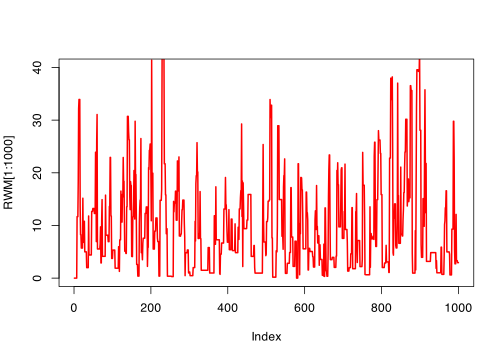
\includegraphics[keepaspectratio]{index_files/mediabag/lectures/L14-rejection_files/figure-pdf/unnamed-chunk-3-1.pdf}}

By rejecting lots of proposals with values near 0, we turned the
unimodal (``one hump'')proposal distribution
\(Y \sim \operatorname{N}(0,1)\) into this interesting bimodal (``two
hump'') distribution.

Let's explain line 3 more carefully. We want to accept a proposal \(x\)
with probability \(\sin^2 x\). We saw in Lecture 12 that we can simulate
a Bernoulli\((p)\) distribution by taking the value 1 is \(U \leq p\)
and taking 0 if \(U > p\). So in line 3, we are accepting each proposed
sample \(x_i\) if a standard uniform variate \(u_i\) satisfies
\(u_i \leq \sin^2 x_i\).

In this example, we found we accepted about 430,000 samples.

\end{example}

In this example, we managed to sample from the PDF in
Equation~\ref{eq-distprop},
\[ f(x) = \frac{1}{Z}\,\exp\big(-\tfrac12x^2\big)\,(\sin^2 x) ,\] even
though we never found out what the normalising constant \(Z\) was. This
idea -- that we can sample from a distribution even if we only know it
up to a multiplicative constant -- is a very important one that will
come up a lot later in this module.

We won't go into that idea deeply now, but we briefly mention that it is
very important in Bayesian statistics. In Bayesian statistics, the
posterior distribution is often known only up to proportionality. That's
because we have \begin{align}
\text{posterior} &\propto \text{prior}\times\text{likelihood} \\
\pi(\theta \mid x) &\propto\, \pi(x) \times p(x \mid \theta)
\end{align} It's often very difficult to find the normalising constant
in this expression -- indeed, it can be impossible in practice. So being
able to sample from such a posterior distribution without finding the
constant is very important for Bayesian statisticians.

\section{How many samples?}\label{how-many-samples}

We have mentioned that the downside of rejection sampling is that we may
have to take lots of proposed samples to get enough accepted ones. Or,
conversely, we may not get enough accepted samples from a fixed number
of proposed samples. Remember that the accuracy of Monte Carlo
estimation, for example, depends on how many (accepted) samples we get
-- the mean-square error scales like \(1/n\) and the root-mean-square
error like \(1/\sqrt{n}\). So it's important to be able to get a lot of
accepted samples \(n\).

Let's examine these questions a bit closer. Write
\(a = \mathbb P(\text{accept})\) for the unconditional probability a
proposal gets accepted (that is, the a priori acceptance probability,
before we have seen the value \(Y = x\) of the proposal). In the
discrete case, this is
\[ a = \mathbb P(\text{accept}) = \sum_x \mathbb P(Y = x)\,\alpha(x) , \]
and in the continuous case this is
\[ a  = \mathbb P(\text{accept}) = \int_{-\infty}^{+\infty} g(x)\,\alpha(x)\,\mathrm{d}x . \]
In both cases, this can be written more succinctly as
\(a = \Exg\alpha(Y)\).

\begin{itemize}
\tightlist
\item
  If we take \(N\) proposals, then the expected number of accepted
  samples is \(n = aN\).
\item
  If we keep taking proposals until getting \(n\) acceptances, then the
  expected number of proposals is \(N = n/a\).
\end{itemize}

If the number of proposals \(N\) is large and the unconditional
acceptance probability \(a\) is not very close to 0, then the actual
number of acceptances will likely be very close to \(aN\). This is
justified by the law of large numbers (and the central limit theorem).
Similarly, if the desired number of acceptances \(n\) is large and \(a\)
is not very close to 0, then the number of required proposals will
likely be very close to \(n/a\). Thus it is in our interest to make
\(a\) as large as we can: this gives us the most acceptances, or
requires the fewest proposals.

We have to be careful when the unconditional acceptance probability is
very close to \(0\). In that case, there can be a lot of variability
required in either the (very small) number of accepted samples or the
(very large) number of required proposals. This unpredictability is
another reason to avoid rejection sampling where the unconditional
acceptance probability \(a\) is very small.

\textbf{Next time.} \emph{We look closer at rejection sampling, and in
particular how we can target rejection sampling at a given distribution
using the ``envelope'' method.}

\textbf{Summary:}

\begin{itemize}
\item
  In rejection sampling, we accept a proposed sample \(Y = x\) with
  probability \(\alpha(x)\).
\item
  If the PDF of a proposed sample is \(g\), then the PDF of an accepted
  sample is proportional to \(\alpha(x) \,g(x)\).
\item
  When the acceptance probability is low, rejection sampling can require
  a lot of proposed samples to get enough accepted samples.
\end{itemize}

\textbf{Read more:}
\href{https://leeds.primo.exlibrisgroup.com/permalink/44LEE_INST/1fj430b/cdi_askewsholts_vlebooks_9781118728031}{Voss,
\emph{An Introduction to Statistical Computing}}, Subsections 1.4.1 and
1.4.3.

\chapter{Envelope rejection sampling
I}\label{envelope-rejection-sampling-i}

Last time, we started looking at rejection sampling. We found that if
you start with a proposal distribution \(Y\) with PDF \(g\), then accept
a proposal \(Y = x\) with probability \(\alpha(x)\), then the PDF \(f\)
of a sample conditional on acceptance satisfies
\(f(x) \propto \alpha(x) g(x)\).

The problem is that this sort of gets the problem backwards. If we pick
a proposal distribution \(g\) and acceptance function \(\alpha\), this
tells us what the sample distribution \(f\) will turn out to be. But we
are interested in the reverse question: If we want to target a
distribution \(f\), what proposal distribution \(g\) and acceptance
function \(\alpha\) do we need to get it?

Today we look at how to do that with the ``envelope'' method.

\section{Sampling under the curve}\label{sampling-under-the-curve}

We will start with a slightly different discussion, to try to motivate
our approach. (If at any point you find this section confuses more than
it helps, you can skip straight to the definition in the next section.)

Consider a PDF \(f\), and draw \(f\) as a curve. We know that \(f(x)\)
is always positive, so this curve is always above the x-axis. We also
know that \(\int_{-\infty}^{+\infty} f(x)\,\mathrm{d}x = 1\), so the
total area under the curve is 1.

Suppose we pick a point under the curve, uniformly at random, and then
look at its x-coordinate \(X\). What is the PDF of \(X\)?

{[}picture{]}

Well, the probability that \(X\) lies in the interval \([a,b]\) is the
probability the point we pick lies in the part of the curve between
\(a\) and \(b\), which is the area of that area divided by the total
area under the curve 1. So
\[ \mathbb P(a \leq X \leq b) = \int_a^b f(x) \,\mathrm{d}x .\] But
that's just the probability associated with the PDF \(f\), so \(X\) has
PDF \(f\).

{[}picture{]}

This gives us a way -- in theory, at least -- to sample from a PDF
\(f\). Simply pick a point at random under the curve, and take its
x-coordinate. Unfortunately, there is no known way to do this directly
in general, so it doesn't really help.

However, suppose we could find a function \(h\) that (a) is positive
everywhere, (b) has finite area under the curve, (c is above \(f\)
everywhere, (d) and that we \emph{could} sample a point under. We could
call such a curve an \textbf{envelope} for \(f\). We could then propose
a point picked at random under the envelope \(h\), reject it if it were
above the curve \(f\), but accept it if it were under the curve \(f\).
An accepted point would be uniform under the curve \(f\), so its
x-coordinate would have PDF \(f\), as required.

{[}picture{]}

But how can we find such an envelope \(h\) we can use?

If the area under the envelope \(h\) is \(c\), with
\(1 \leq c < \infty\) (the area must be at least 1, if the curve is
above \(f\)), then \(h\) must be over the form \(h(x) = cg(x)\) for a
PDF \(g\). But picking the x-coordinate point at random under \(g\) is
just sampling from the random variable that has PDF \(g\). And the
probability that a point with x-coordinate \(x\) from under the envelope
\(cg(x)\) also lies under \(f\) is \(f(x)/cg(x)\), so that would be our
acceptance probability.

This tells us how to perform envelope rejection sampling.

\section{The envelope rejection sampling
algorithm}\label{the-envelope-rejection-sampling-algorithm}

If I lost you during my motivational discussion, now is the time to
switch back on! We are going to set out the steps of the
\textbf{envelope rejection sampling} algorithm.

\begin{itemize}
\item
  \textbf{Goal:} To sample from a random variable \(X\) with PDF \(f\).
\item
  \textbf{We will need:} A random variable \(Y\) with PDF \(g\) that we
  can sample from, and a finite constant \(c\) such that
  \(f(x) \leq cg(x)\) for all \(x\).
\item
  \textbf{Step 1:} Sample a proposal \(Y\) from the PDF \(g\).
\item
  \textbf{Step 2:} Accept the proposal \(Y\) with probability
  \(f(Y) / cg(Y)\); otherwise reject \(Y\). If accepted, \emph{end}. If
  rejected, \emph{go back to Step 1}.
\end{itemize}

Note that for given \(f\) and \(g\), there's no guarantee a finite
constant \(c\) exists such that \(f(x) \leq cg(x)\). Informally, we need
\(g\) to have tails that are ``at least as heavy'' as the tails of
\(f\).

We should check this really does sample from \(f\). We saw last time
that the PDF of a sample had PDF \(f(x) \propto g(x) \,\alpha(x)\).
Here, that is
\[ f(x) \propto g(x)\,\frac{f(x)}{cg(x)} = \frac1c\,f(x) , \] as
required.

In envelope rejection sampling, we reject proposals \(x\) with
probability \(f(x)/cg(x)\). But we saw last time that rejecting samples
is bad -- higher rejection probabilities leave us with fewer accepted
samples (or requiring more proposals to get the same number of accepted
samples). So, for given \(f\) and \(g\), it would be good to pick \(c\)
as small as possible. We must have \(f(x) \leq cg(x)\) for all \(x\), so
we must have \(c \geq f(x) / g(x)\) for all \(x\), and therefore
\(c \geq \sup_x f(x)/g(x)\). (Here, ``sup'' means ``supremum'' -- it's
like the maximum, except allows for the fact the maximum might only be
achieved in a limit, such as \(x \to -\infty\) or \(x \to +\infty\).)
The best possible \(c\), therefore is to take \(c\) to \emph{equal} this
maximum, \(c = \sup_x f(x) / g(x)\), if it's possible to calculate it.

\section{Examples}\label{examples-3}

\begin{example}[]\protect\hypertarget{exm-env1}{}\label{exm-env1}

Consider the Wigner semi-circle distribution with PDF
\[ f(x) = \frac{2}{\pi}\sqrt{1 - x^2} \qquad -1 \leq x \leq 1 . \]

We need to choose the envelope that surrounds the PDF \(f\). Here's one
choice. Let \(Y \sim \operatorname{U}[-1,1]\), which has PDF
\[ g(x) = \tfrac12 \qquad -1 \leq x \leq 1 ,\] which well give a simple
``box'' around \(f\) for the envelope. We can also generate these
samples easily, for example by using the inverse transform
\(Y = 2U - 1\) for \(U \sim \operatorname{U}[0,1]\).

The maximum point of \(f\) is at \(x = 0\), where
\(f(0) = \frac{2}{\pi}\) and \(g(0) = \tfrac12\). So we see that
\(c \geq \frac{4}{\pi}\) will be sufficient to ensure
\(f(x) \leq cg(x)\) for all \(x\), with the box surrounding the
semi-circle. We want to take the smallest possible \(c\), so will take
\(c = \frac{4}{\pi}\), with the box \emph{just} touching the semi-circle
at its top.

\begin{Shaded}
\begin{Highlighting}[]
\NormalTok{pdf }\OtherTok{\textless{}{-}} \ControlFlowTok{function}\NormalTok{(x) (}\DecValTok{2} \SpecialCharTok{/}\NormalTok{ pi) }\SpecialCharTok{*} \FunctionTok{sqrt}\NormalTok{(}\DecValTok{1} \SpecialCharTok{{-}}\NormalTok{ x}\SpecialCharTok{\^{}}\DecValTok{2}\NormalTok{)}
\NormalTok{env }\OtherTok{\textless{}{-}} \ControlFlowTok{function}\NormalTok{(x) (}\DecValTok{4} \SpecialCharTok{/}\NormalTok{ pi) }\SpecialCharTok{*}\NormalTok{ (}\DecValTok{1} \SpecialCharTok{/} \DecValTok{2}\NormalTok{) }\SpecialCharTok{*}\NormalTok{ (}\SpecialCharTok{{-}}\DecValTok{1} \SpecialCharTok{\textless{}=}\NormalTok{ x }\SpecialCharTok{\&}\NormalTok{ x }\SpecialCharTok{\textless{}=} \DecValTok{1}\NormalTok{)}
\end{Highlighting}
\end{Shaded}

\begin{Shaded}
\begin{Highlighting}[]
\FunctionTok{curve}\NormalTok{(}
\NormalTok{  pdf, }\AttributeTok{n =} \DecValTok{1001}\NormalTok{, }\AttributeTok{from =} \SpecialCharTok{{-}}\DecValTok{1}\NormalTok{, }\AttributeTok{to =} \DecValTok{1}\NormalTok{,}
  \AttributeTok{xlim =} \FunctionTok{c}\NormalTok{(}\SpecialCharTok{{-}}\FloatTok{1.5}\NormalTok{, }\FloatTok{1.5}\NormalTok{), }\AttributeTok{ylim =} \FunctionTok{c}\NormalTok{(}\DecValTok{0}\NormalTok{, }\FloatTok{0.8}\NormalTok{), }\AttributeTok{lwd =} \DecValTok{3}\NormalTok{, }\AttributeTok{col =} \StringTok{"blue"}
\NormalTok{)}
\FunctionTok{curve}\NormalTok{(env, }\AttributeTok{n =} \DecValTok{1001}\NormalTok{, }\AttributeTok{add =} \ConstantTok{TRUE}\NormalTok{, }\AttributeTok{lwd =} \DecValTok{2}\NormalTok{, }\AttributeTok{col =} \StringTok{"red"}\NormalTok{)}
\end{Highlighting}
\end{Shaded}

\pandocbounded{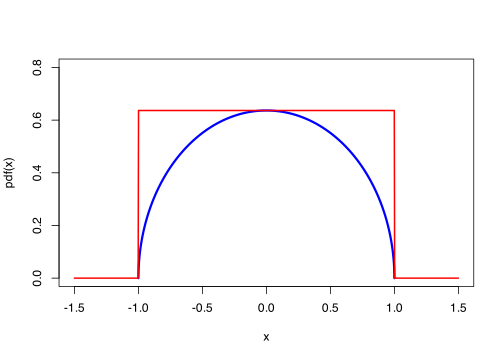
\includegraphics[keepaspectratio]{index_files/mediabag/lectures/L15-envelope-1_files/figure-pdf/semi1-1.pdf}}

In my code, I've set it up so that \texttt{env()} (the envelope
function) is \(c\) times \(g\).

\begin{Shaded}
\begin{Highlighting}[]
\NormalTok{n\_prop }\OtherTok{\textless{}{-}} \FloatTok{1e6}
\NormalTok{props }\OtherTok{\textless{}{-}} \DecValTok{2} \SpecialCharTok{*} \FunctionTok{runif}\NormalTok{(n\_prop) }\SpecialCharTok{{-}} \DecValTok{1}
\NormalTok{accepts }\OtherTok{\textless{}{-}}\NormalTok{ props[}\FunctionTok{runif}\NormalTok{(n\_prop) }\SpecialCharTok{\textless{}=} \FunctionTok{pdf}\NormalTok{(props) }\SpecialCharTok{/} \FunctionTok{env}\NormalTok{(props)]}

\FunctionTok{length}\NormalTok{(accepts)}
\end{Highlighting}
\end{Shaded}

\begin{verbatim}
[1] 785263
\end{verbatim}

\begin{Shaded}
\begin{Highlighting}[]
\FunctionTok{hist}\NormalTok{(accepts, }\AttributeTok{probability =} \ConstantTok{TRUE}\NormalTok{, }\AttributeTok{breaks =} \DecValTok{40}\NormalTok{)}
\FunctionTok{curve}\NormalTok{(pdf, }\AttributeTok{add =} \ConstantTok{TRUE}\NormalTok{, }\AttributeTok{lwd =} \DecValTok{2}\NormalTok{, }\AttributeTok{col =} \StringTok{"blue"}\NormalTok{)}
\end{Highlighting}
\end{Shaded}

\pandocbounded{\includegraphics[keepaspectratio]{index_files/mediabag/lectures/L15-envelope-1_files/figure-pdf/unnamed-chunk-2-1.pdf}}

We see that we accepted about 78\% or 79\% of proposals, and the
histogram is an excellent fit to the semicircle distribution.

\end{example}

\begin{example}[]\protect\hypertarget{exm-env-norm}{}\label{exm-env-norm}

Suppose we want to sample from the ``half-normal'' distribution
\[ f(x) = \sqrt\frac{2}{\pi} \exp\big(\tfrac12 x^2\big) \qquad x \geq 0 . \]
Let's take \(Y \sim \operatorname{Exp}(1)\) with
\(g(x) = \mathrm{e}^{-x}\). We know this can be easily sampled from,
using the inverse transform \(Y = - \log U\). The exponential also has
fatter tails than the normal, so this should work.

To find an appropriate \(c\), we consider
\[ \frac{f(x)}{g(x)} = \frac{\sqrt\frac{2}{\pi} \exp(\tfrac12 x^2)}{\exp(-x)} = \sqrt\frac{2}{\pi} \exp \big(-\tfrac12 x^2 + x\big) . \]
This is maximised where \(-\tfrac12 x^2 + x\) is maximised which (by
differentiating and setting equal to 0) is at \(x = 1\). So we take the
best possible \(c\), which is
\[ c = \frac{f(1)}{g(1)} = \sqrt\frac{2}{\pi} \exp\big(-\tfrac12 + 1\big) = \sqrt\frac{2\mathrm{e}}{\pi} . \]

\begin{Shaded}
\begin{Highlighting}[]
\NormalTok{pdf }\OtherTok{\textless{}{-}} \ControlFlowTok{function}\NormalTok{(x) }\FunctionTok{sqrt}\NormalTok{(}\DecValTok{2} \SpecialCharTok{/}\NormalTok{ pi) }\SpecialCharTok{*} \FunctionTok{exp}\NormalTok{(}\SpecialCharTok{{-}}\NormalTok{x}\SpecialCharTok{\^{}}\DecValTok{2} \SpecialCharTok{/} \DecValTok{2}\NormalTok{)}
\NormalTok{env }\OtherTok{\textless{}{-}} \ControlFlowTok{function}\NormalTok{(x) }\FunctionTok{sqrt}\NormalTok{(}\DecValTok{2} \SpecialCharTok{*} \FunctionTok{exp}\NormalTok{(}\DecValTok{1}\NormalTok{) }\SpecialCharTok{/}\NormalTok{ pi) }\SpecialCharTok{*} \FunctionTok{exp}\NormalTok{(}\SpecialCharTok{{-}}\NormalTok{x)}
\end{Highlighting}
\end{Shaded}

\begin{Shaded}
\begin{Highlighting}[]
\FunctionTok{curve}\NormalTok{(}
\NormalTok{  pdf, }\AttributeTok{n =} \DecValTok{1001}\NormalTok{, }\AttributeTok{from =} \DecValTok{0}\NormalTok{, }\AttributeTok{to =} \DecValTok{4}\NormalTok{,}
  \AttributeTok{xlim =} \FunctionTok{c}\NormalTok{(}\DecValTok{0}\NormalTok{, }\DecValTok{3}\NormalTok{), }\AttributeTok{ylim =} \FunctionTok{c}\NormalTok{(}\DecValTok{0}\NormalTok{, }\FloatTok{1.32}\NormalTok{), }\AttributeTok{lwd =} \DecValTok{3}\NormalTok{, }\AttributeTok{col =} \StringTok{"blue"}
\NormalTok{)}
\FunctionTok{curve}\NormalTok{(env, }\AttributeTok{n =} \DecValTok{1001}\NormalTok{, }\AttributeTok{from =} \DecValTok{0}\NormalTok{, }\AttributeTok{to =} \DecValTok{4}\NormalTok{, }\AttributeTok{add =} \ConstantTok{TRUE}\NormalTok{, }\AttributeTok{lwd =} \DecValTok{2}\NormalTok{, }\AttributeTok{col =} \StringTok{"red"}\NormalTok{)}
\end{Highlighting}
\end{Shaded}

\pandocbounded{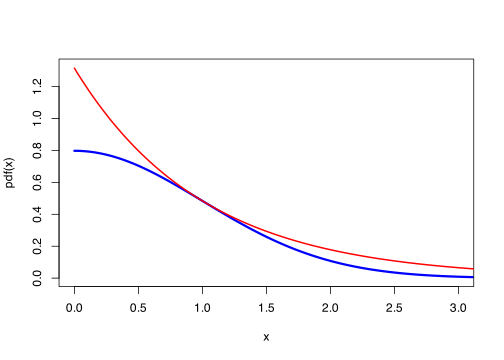
\includegraphics[keepaspectratio]{index_files/mediabag/lectures/L15-envelope-1_files/figure-pdf/halfnorm-1.pdf}}

\begin{Shaded}
\begin{Highlighting}[]
\NormalTok{n\_prop }\OtherTok{\textless{}{-}} \FloatTok{1e6}
\NormalTok{props }\OtherTok{\textless{}{-}} \SpecialCharTok{{-}}\FunctionTok{log}\NormalTok{(}\FunctionTok{runif}\NormalTok{(n\_prop))}
\NormalTok{accepts }\OtherTok{\textless{}{-}}\NormalTok{ props[}\FunctionTok{runif}\NormalTok{(n\_prop) }\SpecialCharTok{\textless{}=} \FunctionTok{pdf}\NormalTok{(props) }\SpecialCharTok{/} \FunctionTok{env}\NormalTok{(props)]}

\FunctionTok{length}\NormalTok{(accepts)}
\end{Highlighting}
\end{Shaded}

\begin{verbatim}
[1] 760751
\end{verbatim}

\begin{Shaded}
\begin{Highlighting}[]
\FunctionTok{hist}\NormalTok{(accepts, }\AttributeTok{probability =} \ConstantTok{TRUE}\NormalTok{, }\AttributeTok{breaks =} \DecValTok{40}\NormalTok{)}
\FunctionTok{curve}\NormalTok{(pdf, }\AttributeTok{add =} \ConstantTok{TRUE}\NormalTok{, }\AttributeTok{lwd =} \DecValTok{2}\NormalTok{, }\AttributeTok{col =} \StringTok{"blue"}\NormalTok{)}
\end{Highlighting}
\end{Shaded}

\pandocbounded{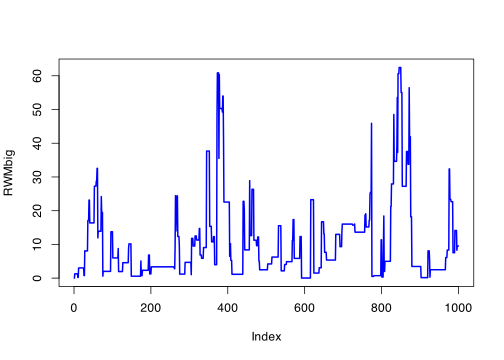
\includegraphics[keepaspectratio]{index_files/mediabag/lectures/L15-envelope-1_files/figure-pdf/unnamed-chunk-4-1.pdf}}

We accept roughly 760,000 proposals, and get an excellent fit to the
half-normal distribution.

\end{example}

\textbf{Next time.} \emph{We study envelope rejection sampling more
closely, and complete this part of the module on random number
generation}

\textbf{Summary:}

\begin{itemize}
\item
  For envelope rejection sampling from a PDF \(f\), we need a PDF \(g\)
  from which we can sample and a constant \(c\) such that
  \(f(x) \leq cg(x)\) for all \(x\).
\item
  We propose samples from \(g\), and accept a proposal \(x\) with
  probability \(f(x) / cg(x)\).
\item
  To keep the acceptance probability high, we want to pick \(c\) as
  small as possible.
\end{itemize}

\textbf{Read more:}
\href{https://leeds.primo.exlibrisgroup.com/permalink/44LEE_INST/1fj430b/cdi_askewsholts_vlebooks_9781118728031}{Voss,
\emph{An Introduction to Statistical Computing}}, Subsections 1.4.2.

\chapter{Envelope rejection sampling
II}\label{envelope-rejection-sampling-ii}

Last time we discussed envelope rejection sampling. The process was the
following:

\begin{itemize}
\item
  \textbf{Goal:} To sample from a random variable \(X\) with PDF \(f\).
\item
  \textbf{We will need:} A random variable \(Y\) with PDF \(g\) that we
  can sample from, and a finite constant \(c\) such that
  \(f(x) \leq cg(x)\) for all \(x\).
\item
  \textbf{Step 1:} Sample a proposal \(Y\) from the PDF \(g\).
\item
  \textbf{Step 2:} Accept the proposal \(Y\) with probability
  \(f(Y) / cg(Y)\).
\end{itemize}

While we covered the most important facts about envelope rejection
sampling last time, there are a few quick matters to mop up today.

\section{Acceptance probability}\label{acceptance-probability-1}

Conditional on seeing a proposal \(Y = x\), we saw that the acceptance
probability is \[ \alpha(x) = \frac{f(x)}{cg(x)} . \] For any particular
\(x\), this increases as \(c\) decreases, which is why we wanted \(c\)
as small as possible, subject to \(f(x) \leq cg(x)\) for all \(x\).

But what is the overall acceptance probability -- unconditionally,
before we've seen the value of the proposal?

As we saw before, the overall acceptance probability is
\[ \operatorname{\mathbb E}\alpha(Y) = \int_{-\infty}^{+\infty} \alpha(x)\,g(x)\,\mathrm{d}x . \]
Substituting in our value of \(\alpha\), we have
\[ \operatorname{\mathbb E}\alpha(Y) = \int_{-\infty}^{+\infty} \frac{f(x)}{cg(x)}\,g(x)\,\mathrm{d}x = \frac{1}{c} \int_{-\infty}^{+\infty} f(x) \, \mathrm{d}x  = \frac{1}{c} , \]
since the integral of PDF \(f\) is 1. Thus the unconditional acceptance
probability is therefore \(1/c\). To put it another way, the expected
number of proposals per acceptance is \(c\).

This is another even more direct reason why we should want to take \(c\)
as small as possible.

\begin{example}[]\protect\hypertarget{exm-acc-vals}{}\label{exm-acc-vals}

In Example~\ref{exm-env1}, we took \(c = \frac{4}{\pi}\), so
\(1/c = \frac{\pi}{4} = 0.785\). We saw that we accepted 78\% or 79\% of
the proposals.

In Example~\ref{exm-env-norm}, we took
\[c = \sqrt\frac{2\mathrm{e}}{\pi} \qquad \frac{1}{c} = \sqrt{\frac{\pi}{2\mathrm{e}}} = 0.760.\]
We saw that we accepted about 76\% of proposals.

\end{example}

\section{Unnormalised measures}\label{unnormalised-measures}

We briefly mentioned in Lecture 14 that it can be useful to be able to
be able to sample from PDFs even when we only know the PDF up to
proportionality, and that this is particularly useful in Bayesian
statistics.

Suppose we want to sample from a PDF \[ f(x) = \frac{1}{Z}\,\mu(x) , \]
where the \textbf{measure} \(\mu\) is known, but the normalising
constant \[ Z = \int_{-\infty}^{+\infty}\mu(x) \,\mathrm{d}x \] is
unknown (but finite). Can we do this with envelope rejection sampling?

The answer is yes -- and algorithm is basically exactly the same, just
with \(f\) replaced by \(\mu\).

\begin{itemize}
\item
  \textbf{Goal:} To sample from a random variable \(X\) with PDF
  proportional to the measure \(\mu\).
\item
  \textbf{We will need:} A random variable \(Y\) with PDF \(g\) that we
  can sample from, and a finite constant \(c\) such that
  \(\mu(x) \leq cg(x)\) for all \(x\).
\item
  \textbf{Step 1:} Sample a proposal \(Y\) from the PDF \(g\).
\item
  \textbf{Step 2:} Accept the proposal \(Y\) with probability
  \(\mu(Y) / cg(Y)\); otherwise reject \(Y\). If accepted, \emph{end}.
  If rejected, \emph{go back to Step 1}.
\end{itemize}

To check that this still works, we remember that the accepted PDF is
proportional to
\[ \alpha(x) \,g(x) = \frac{\mu(x)}{cg(x)}\,g(x) = \frac{1}{c} \mu(x) \propto \mu(x) \propto f(x) . \]

In the unnormalised case, \(1/c\) is only proportional to, not directly
equal to, the unconditional acceptance probability. So we still want
\(c\) as small as possible, but can't give it a direct interpretation as
an acceptance probability.

\begin{example}[]\protect\hypertarget{exm-mises}{}\label{exm-mises}

The \textbf{von Mises distribution} is a distribution on \([0, 2\pi)\)
with PDF \[f(x) \propto \mu(x) = \exp\big(\kappa \cos (x-m)\big), \]for
some parameters \(m \in [0, 2\pi)\) and \(\kappa \geq 0\). The von Mises
distribution is used to model data on a circle, with \(x\) being the
angle around the circle. Circular data might be a compass direction
(north/south/east/west), or a time of day (with the circle representing
the hours from midnight to midnight). The von Mises distribution is sort
of a ``circular equivalent'' of the normal distribution on the line,
with \(m\) being the mean value and \(\kappa\) playing a similar role
\(1/\sigma^2\). There is no closed form for the constant of
proportionality.

We wish to sample from the von Mises distribution with \(m = 0\) and
\(\kappa = 2\), where the unnormalised measure is
\(\mu(x) = \exp(2\cos x)\). We choose the uniform distribution
\(g(x) = \frac{1}{2\pi}\) on \([0, 2\pi)\) for our envelope, which we
can easily sample from as \(Y = 2\pi U\). To choose \(c\), we note that
the maximum of \(\mu(x)\) is at \(x = 0\), where it takes the value
\(\exp(2)\). So we take \(c = \mu(0)/g(0) = 2\pi\mathrm{e}^2\).

\begin{Shaded}
\begin{Highlighting}[]
\NormalTok{meas }\OtherTok{\textless{}{-}} \ControlFlowTok{function}\NormalTok{(x) }\FunctionTok{exp}\NormalTok{(}\DecValTok{2} \SpecialCharTok{*} \FunctionTok{cos}\NormalTok{(x))}
\NormalTok{env  }\OtherTok{\textless{}{-}} \ControlFlowTok{function}\NormalTok{(x) }\DecValTok{2} \SpecialCharTok{*}\NormalTok{ pi }\SpecialCharTok{*} \FunctionTok{exp}\NormalTok{(}\DecValTok{2}\NormalTok{) }\SpecialCharTok{*}\NormalTok{ (}\DecValTok{1} \SpecialCharTok{/}\NormalTok{ (}\DecValTok{2} \SpecialCharTok{*}\NormalTok{ pi)) }\SpecialCharTok{*}\NormalTok{ (x }\SpecialCharTok{\textless{}=} \DecValTok{2} \SpecialCharTok{*}\NormalTok{ pi)}
\end{Highlighting}
\end{Shaded}

\begin{Shaded}
\begin{Highlighting}[]
\FunctionTok{curve}\NormalTok{(}
\NormalTok{  meas, }\AttributeTok{n =} \DecValTok{1001}\NormalTok{, }\AttributeTok{from =} \DecValTok{0}\NormalTok{, }\AttributeTok{to =} \DecValTok{2} \SpecialCharTok{*}\NormalTok{ pi,}
  \AttributeTok{lwd =} \DecValTok{3}\NormalTok{, }\AttributeTok{col =} \StringTok{"blue"}
\NormalTok{)}
\FunctionTok{curve}\NormalTok{(env, }\AttributeTok{n =} \DecValTok{1001}\NormalTok{, }\AttributeTok{add =} \ConstantTok{TRUE}\NormalTok{, }\AttributeTok{lwd =} \DecValTok{2}\NormalTok{, }\AttributeTok{col =} \StringTok{"red"}\NormalTok{)}
\end{Highlighting}
\end{Shaded}

\pandocbounded{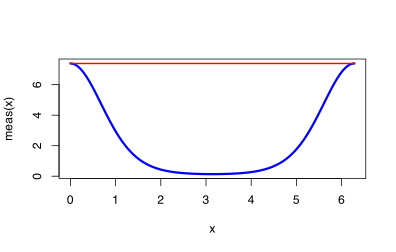
\includegraphics[keepaspectratio]{index_files/mediabag/lectures/L16-envelope-2_files/figure-pdf/vonmises-1.pdf}}

(This graph might look a little odd, but remember that \(0\) and
\(2\pi\) are the same part of the circle, so this measure takes its
largest values around that ``join''.)

\begin{Shaded}
\begin{Highlighting}[]
\NormalTok{n\_prop }\OtherTok{\textless{}{-}} \FloatTok{1e6}
\NormalTok{props }\OtherTok{\textless{}{-}} \DecValTok{2} \SpecialCharTok{*}\NormalTok{ pi }\SpecialCharTok{*}\NormalTok{ (}\FunctionTok{runif}\NormalTok{(n\_prop))}
\NormalTok{accepts }\OtherTok{\textless{}{-}}\NormalTok{ props[}\FunctionTok{runif}\NormalTok{(n\_prop) }\SpecialCharTok{\textless{}=} \FunctionTok{meas}\NormalTok{(props) }\SpecialCharTok{/} \FunctionTok{env}\NormalTok{(props)]}

\FunctionTok{length}\NormalTok{(accepts)}
\end{Highlighting}
\end{Shaded}

\begin{verbatim}
[1] 307849
\end{verbatim}

\begin{Shaded}
\begin{Highlighting}[]
\FunctionTok{hist}\NormalTok{(accepts, }\AttributeTok{probability =} \ConstantTok{TRUE}\NormalTok{, }\AttributeTok{breaks =} \DecValTok{2} \SpecialCharTok{*}\NormalTok{ pi }\SpecialCharTok{*}\NormalTok{ (}\DecValTok{0}\SpecialCharTok{:}\DecValTok{30}\NormalTok{) }\SpecialCharTok{/} \DecValTok{30}\NormalTok{)}
\FunctionTok{curve}\NormalTok{(}\FunctionTok{meas}\NormalTok{(x) }\SpecialCharTok{/} \FloatTok{14.3}\NormalTok{, }\AttributeTok{add =} \ConstantTok{TRUE}\NormalTok{, }\AttributeTok{lwd =} \DecValTok{2}\NormalTok{, }\AttributeTok{col =} \StringTok{"blue"}\NormalTok{)}
\end{Highlighting}
\end{Shaded}

\pandocbounded{\includegraphics[keepaspectratio]{index_files/mediabag/lectures/L16-envelope-2_files/figure-pdf/unnamed-chunk-2-1.pdf}}

We accepted about 31\% of proposals.

\end{example}

\section{Summary of Part II}\label{summary-of-part-ii}

This completes our study of random number generation. This would be a
good time to summarise what we have learned.

First we discussed generating randomness.

\begin{itemize}
\item
  We can generate random numbers uniform on \([0,1]\) through true
  physical randomness or by a pseudorandom number generator.
\item
  LCGs are one type of pseudorandom number generator. An LCG is a
  recurrence \(x_{n+1} = (ax_n + c) \bmod m\).
\item
  Conditions for an LCG to have full period of \(m\) are given by the
  Hull--Dobell theorem: if \(m\) is a power of 2, then we need \(c\) to
  be odd and \(a\) to be \(1 \bmod 4\). {[}\textbf{Note:} \emph{In the
  lecture, I wrongly said we need \(c\) to be even; in fact, we need
  \(c\) to be odd.}{]}
\end{itemize}

Then we discussed manipulating standard uniform samples into other
distributions.

\begin{itemize}
\item
  The inverse transform method uses the cumulative distribution
  function: set \(U = F(X)\) and invert to make \(X\) the subject.
\item
  Discrete random variables can be simulated by splitting up the
  intervals \([0,1]\) into segments of length \(p(x_i)\), then seeing
  which segment \(U\) falls into.
\item
  Two normal distributions can be sampled using the Box--Muller theorem
  and polar coordinates. Let \(R\) be Rayleigh distributed, \(\Theta\)
  be uniform on \([0, 2\pi)\), then set \(X = R \cos \Theta\) and
  \(Y = R \sin \Theta\).
\item
  We can also get different distributions by accepting a proposed sample
  \(Y = x\) from \(g\) with probability \(\alpha(x)\). The PDF of an
  accepted sample is \(f(x) \propto \alpha(x)\,g(x)\).
\item
  Envelope rejection sampling is a way to target rejection sampling a
  PDF \(f\), by choosing an ``envelope'' \(cg(x)\), and accepting a
  sample from \(g\) with probability \(f(x)/cg(x)\).
\item
  Rejection sampling works best when the acceptance probability is made
  as large as possible.
\end{itemize}

\textbf{Next time.} \emph{We begin our study on MCMC: Markov chain Monte
Carlo.}

\textbf{Summary:}

\begin{itemize}
\item
  Envelope rejection sampling with envelope \(cg(x)\) has unconditional
  acceptance probability \(1/c\).
\item
  Envelope rejection sampling works even if the desired distribution is
  only know up to a proportionality constant.
\end{itemize}

\textbf{Read more:}
\href{https://leeds.primo.exlibrisgroup.com/permalink/44LEE_INST/1fj430b/cdi_askewsholts_vlebooks_9781118728031}{Voss,
\emph{An Introduction to Statistical Computing}}, Subsections 1.4.2.

\chapter*{Problem Sheet 3}\label{P3}
\addcontentsline{toc}{chapter}{Problem Sheet 3}

\markboth{Problem Sheet 3}{Problem Sheet 3}

\textbf{\hyperref[P3-sols]{Full solutions}} are now available.

This is Problem Sheet 3, which covers material from Lectures 12 to 16.
You should work through all the questions on this problem sheet in
advance of the problems class, which takes place in the lecture of
\textbf{Thursday 13 November}.

This problem sheet is to help you practice material from the module and
to help you check your learning. It is \emph{not} for formal assessment
and does not count towards your module mark.

If you want some brief informal feedback on \textbf{Question 3 parts (a)
and (b) and Question 6} (marked ★), you should submit your work
electronically through Gradescope via the module's Minerva page by
\textbf{1400 on Tuesday 11 November}. (If you hand-write solutions on
paper, the easiest way to scan-and-submit that work is using the
Gradescope app on your phone.) I will return some brief comments on your
those two questions by the problems class on Thursday 13 November.
Because this informal feedback, and not part of the official assessment,
I cannot accept late work for any reason -- but I am always happy to
discuss any of your work on any question in my office hours.

Full solutions will be released on Friday 14 November.

\part{MCMC}

\chapter{Markov chains in discrete
space}\label{markov-chains-in-discrete-space}

\[ \]

\section{Markov chains and MCMC}\label{markov-chains-and-mcmc}

In the first part of this module, we looked at Monte Carlo methods,
where we estimated \(\theta = \Exg\phi(X)\) by
\[ \widehat{\theta}_n = \frac{1}{n} \sum_{i=1}^n \phi(X_i) \]. To do
this, we need samples \(X_1, X_2, \dots, X_n\) that (a) come from the
exactly the same distribution as \(X\), and (b) are independent of each
other.

We can often manage to generate random samples like these if \(X\) has a
relatively simple distributions \(X\): for example, we can use the
inverse transform method or envelope rejection sampling (or a built-in R
function). These simple distributions tend to be one-dimensional
distributions, sometimes with a simple dependence on one parameter.

However, these random number generation methods are often not available
when dealing with very complex distributions \(X\). For example, these
might not be one-dimensional but rather living in some very
high-dimensional space. Or they might depend on many parameters -- and
those parameters might themselves be drawn from random distributions (a
so-called ``hierarchical model'').

For more complicated distributions, we can make progress by loosening
the assumption that \(X_1, X_2, \dots, X_n\) are perfect IID copies of
\(X\).

\begin{itemize}
\item
  Rather than the \(X_i\) having \emph{exactly} the same distribution as
  \(X\), we might be willing for them to have approximately the same
  distribution as \(X\), or to converge to that distribution as \(i\)
  gets large.
\item
  Rather than having the \(X_i\) be completely independent, we could let
  them have some dependence; but we will want to set things up so that
  we limit the dependence so there is only ``light'' dependence and so
  that we understand the dependence structure well.
\end{itemize}

The way will do this is to allow \(X_1, X_2, \dots\) to be a random
process (or ``stochastic'' process) that has a particular dependence
structure known as the \textbf{Markov property}. Such a process is known
as a \textbf{Markov chain}. Random variables in Markov chains can be
shown (under certain conditions) to tend to a certain distribution -- we
will want to set things up so that that ``limiting distribution'' is the
distribution \(X\) we want to sample from.

Using a Monte Carlo estimator where the samples \(X_1, X_2, \dots\) are
not IID but rather form a Markov chain is known as \textbf{Markov chain
Monte Carlo} -- almost always referred to by the abbreviation
\textbf{MCMC}. And ``MCMC'' has become to be used more widely for
generating samples according to a Markov chain even if those samples
aren't necessarily used for Monte Carlo estimation. MCMC is one of the
most important ideas in statistics in the second-half of the 20th and in
the 21st centuries, and is especially important in Bayesian statistics.

In this part of the of the module, we will study MCMC in depth. We will
take a brief tour through the theory of Markov chains, then talk about
how to use the output of a Markov chain for Monte Carlo estimation. We
will look specifically at the \textbf{Metropolis--Hastings algorithm},
which is one way of setting up a Markov chain to have a specific
distribution as its limiting distribution, and has some properties in
common with rejection sampling ideas we have already seen.

The schedule will be:

\begin{itemize}
\item
  Today and Lecture 18: Theory of Markov chains in discrete space
\item
  Lecture 19: Metropolis--Hastings algorithm in discrete space
\item
  Lecture 20: Theory of Markov chains in continuous space
\item
  Lecture 21: Metropolis--Hastings algorithm in continuous space
\item
  Lectures 22 and 23: MCMC in practice (including for Bayesian
  statistics).
\end{itemize}

Some of you may have studied Markov chains before -- for example, in the
Leeds second-year module
\href{https://mpaldridge.github.io/math2750/}{MATH2750 Introduction to
Markov Processes}. If so, you should find that today and the next
lecture are just a brief reminder of things you already know, but the
rest of the material is likely to be new. However, I will not assume any
pre-existing knowledge of Markov chains, and will teach you everything
you need to know for this module.

\section{Introduction to Markov
chains}\label{introduction-to-markov-chains}

A \textbf{Markov chain} in discrete time \(i = 1, 2, \dots\) and
discrete space \(\mathcal S\) is a sequence of random variables
\((X_1, X_2, X_3, \dots)\) taking values in \(\mathcal S\). The random
variables are not independent, but the dependence of any of the random
variables is limited to just the random variable before it in the list.
That is, the next state \(X_{i+1}\) can depend on on the current state
\(X_i\); but, given the current state \(X_i\), it has no further
dependence on the past states \(X_{i-1}, X_{i-2}, \dots, X_2, X_1\).
This is known as the ``Markov property''.

Think of playing a simple board game where you roll a dice and move that
many squares along the board. Let \(X_i\) be the current square you are
on. The the next square you land on, \(X_{i+1}\):

\begin{itemize}
\item
  is random -- because it depends on the roll of the dice;
\item
  depends on which square \(X_i\) you are on now -- because the value of
  dice roll will be added to your current square;
\item
  \emph{given} the square \(X_i\) you are on now, it doesn't depend
  which sequence of squares \(X_1, X_2, \dots, X_{i-1}\) you previously
  landed on to get there.
\end{itemize}

\begin{definition}[]\protect\hypertarget{def-markov}{}\label{def-markov}

A sequence of random variables \((X_i) = (X_1, X_2, \dots)\) taking
values in a countable state space \(\mathcal S\) is said to be a
\textbf{Markov chain} or to have the \textbf{Markov property} if
\[ \mathbb P(X_{i+1} = x_{i+1} \mid X_i = x_i, X_{i-1} = x_{i=1}, \dots, X_1 = x_1) 
= \mathbb P(X_{i+1} = x_{i+1} \mid X_i = x_i)\] for all
\(i = 1, 2, \dots\) and for all
\(x_1, \dots, x_{i-1}, x_{i}, x_{i+1} \in \mathcal S\) such that the
conditional probability is defined.

\end{definition}

\begin{example}[]\protect\hypertarget{exm-2state}{}\label{exm-2state}

Consider a simple model of an unreliable printer:

\begin{itemize}
\item
  On day 1, the printer is working.
\item
  If the printer is working, then the next day there is a 90\% chance it
  is still working, but a 10\% chance it has broken.
\item
  If the printer is broken, then the next day there is a 50\% chance it
  has been mended, but a 50\% chance it is still broken.
\end{itemize}

We can model this as a Markov chain on the state space
\(\mathcal S = \{1, 2\}\), where state 1 denotes that the printer is
working and state 2 denotes that the printer is working. We have
\begin{align}
\mathbb P(X_{i+1} = 1 \mid X_i = 1) &= 0.9 & \mathbb P(X_{i+1} = 2 \mid X_i = 1) &= 0.1 \\
\mathbb P(X_{i+1} = 1 \mid X_i = 2) &= 0.5 & \mathbb P(X_{i+1} = 2 \mid X_i = 2) &= 0.5.
\end{align}

\end{example}

\begin{example}[]\protect\hypertarget{exm-rw}{}\label{exm-rw}

Consider the \textbf{simple random walk} on \(\mathcal S = \mathbb Z\).
We start at \(X_1 = 0\). At each time step, we move up 1 with
probability \(p\) and down one with probability \(q = 1-p\); so
\[ \mathbb P(X_{i+1} = y \mid X_i = x) = \begin{cases} p & \text{ if }y = x+1 \\ q & \text{ if }y = x-1 \\
0 & \text{ otherwise}. \end{cases} \]

If \(p = q = \tfrac12\), this is called the \textbf{simple symmetric
random walk}.

We can also write this as
\begin{equation}\phantomsection\label{eq-rw}{ X_{i+1} = X_i + Z_i , }\end{equation}
where the \(Z_i\) are IID with distribution
\[ Z_i = \begin{cases} +1 & \text{ with probability } p \\ -1 & \text{ with probability } q. \end{cases} \]
Any Markov chain with the structure Equation~\ref{eq-rw} for an IID
sequence \((Z_i)\) is called a \textbf{random walk}. If the \(Z_i\) are
symmetric, in that \(\mathbb P(Z_i = +z) = \mathbb P(Z_i = -z)\) for all
\(z\), then it is a \textbf{symmetric random walk}.

\end{example}

In both the Markov chains we have looked at -- and, indeed, all the
Markov chains we will ever look at -- the \textbf{transition
probability} \(p(x, y) = \mathbb P(X_{i+1} = y \mid X_i = x)\) was the
same for all \(i\). That is, the probability \(p(x, y)\) of moving from
\(x\) to \(y\) does not depend on which timestep \(i\) we are at. This
is called being \textbf{time homogeneous}.

Once we have the notation \(p(x, y)\) for the transition probability, it
will in fact be useful to write them in a matrix
\(\mathsf P = (p(x,y))\), called the \textbf{transition matrix}.

For the two-state ``unreliable printer'' Markov chain, the transition
matrix is
\[ \mathsf P = \begin{pmatrix} 0.9 & 0.1 \\ 0.5 & 0.5 \end{pmatrix} . \]

For the simple random walk, the transition matrix is the ``infinite
matrix'' \[ \mathsf P = \begin{pmatrix}
 \smash\ddots      & \smash\ddots & \phantom{\smash\ddots}  &  \phantom{\smash\ddots}  & \phantom{\smash\ddots} & \phantom{\smash\ddots} \\
\smash\ddots &  0     & p &        & \\
       & q      & 0 & p      & \\
       &        & q & 0      & p \\
       &        &   & q & 0 & \smash\ddots \\
       &        &   &  & \smash\ddots &  \smash\ddots       \end{pmatrix} \]
This has 0s down the diagonal (representing the probability 0 of staying
still), \(p\) one place to the right of the diagonal (representing the
probability of moving up 1), and \(q\) one place to the left of the
diagonal (representing the probability of moving down 1). Blank spaces
in this matrix denotes 0s.

The \(x\)th row of a transition matrix represents the probabilities of
moving from \(x\) to each of the other states. Thus each row must
consist of non-negative numbers that add up to 1, as is the case in both
of our examples.

\section{Simulation of Markov chains}\label{simulation-of-markov-chains}

We can take \(n\) samples from a finite-state Markov chain in R with the
following function. In the function \texttt{rmarkov()}, \texttt{n} is
the number of samples (or steps) to take, \texttt{trans} is the
transition matrix \(\mathsf P\), and \texttt{initial} is the initial
state \(X_1\).

\begin{Shaded}
\begin{Highlighting}[]
\NormalTok{rmarkov }\OtherTok{\textless{}{-}} \ControlFlowTok{function}\NormalTok{(n, trans, initial) \{}
\NormalTok{  states }\OtherTok{\textless{}{-}} \FunctionTok{nrow}\NormalTok{(trans)}
\NormalTok{  MC }\OtherTok{\textless{}{-}} \FunctionTok{rep}\NormalTok{(}\DecValTok{0}\NormalTok{, n)}
  
\NormalTok{  MC[}\DecValTok{1}\NormalTok{] }\OtherTok{\textless{}{-}}\NormalTok{ initial}
  \ControlFlowTok{for}\NormalTok{ (i }\ControlFlowTok{in} \DecValTok{1}\SpecialCharTok{:}\NormalTok{(n }\SpecialCharTok{{-}} \DecValTok{1}\NormalTok{)) MC[i }\SpecialCharTok{+} \DecValTok{1}\NormalTok{] }\OtherTok{\textless{}{-}} \FunctionTok{sample}\NormalTok{(states, }\DecValTok{1}\NormalTok{, }\AttributeTok{prob =}\NormalTok{ trans[MC[i], ])}
  
  \FunctionTok{return}\NormalTok{(MC)}
\NormalTok{\}}
\end{Highlighting}
\end{Shaded}

The key line is the \texttt{for} loop in the penultimate line. Here, the
next state \(X_{i+1}\) is chosen by sampling one state from the state
space with probabilities according to the current state's row of the
transition matrix.

\begin{example}[]\protect\hypertarget{exm-2state2}{}\label{exm-2state2}

Let's simulate the two-state broken printer Markov chain from
Example~\ref{exm-2state}.

\begin{Shaded}
\begin{Highlighting}[]
\NormalTok{trans }\OtherTok{\textless{}{-}} \FunctionTok{matrix}\NormalTok{(}\FunctionTok{c}\NormalTok{(}\FloatTok{0.9}\NormalTok{, }\FloatTok{0.1}\NormalTok{, }\FloatTok{0.5}\NormalTok{, }\FloatTok{0.5}\NormalTok{), }\DecValTok{2}\NormalTok{, }\DecValTok{2}\NormalTok{, }\AttributeTok{byrow =} \ConstantTok{TRUE}\NormalTok{)}
\NormalTok{initial }\OtherTok{\textless{}{-}} \DecValTok{1}
\NormalTok{MC }\OtherTok{\textless{}{-}} \FunctionTok{rmarkov}\NormalTok{(}\DecValTok{80}\NormalTok{, trans, initial)}
\FunctionTok{plot}\NormalTok{(MC, }\AttributeTok{col =} \StringTok{"blue"}\NormalTok{, }\AttributeTok{lwd =} \DecValTok{2}\NormalTok{, }\AttributeTok{type =} \StringTok{"b"}\NormalTok{)}
\end{Highlighting}
\end{Shaded}

\pandocbounded{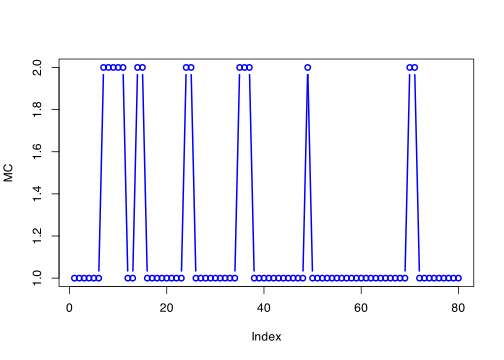
\includegraphics[keepaspectratio]{index_files/mediabag/lectures/L17-markov-intro_files/figure-pdf/r2state-1.pdf}}

In the first line, we entered a \(2 \times 2\) matrix using the code
\texttt{matrix(P,\ 2,\ 2)}, where \texttt{P} was a vector of length
\(2 \times 2 = 4\). R default is to fill up the matrix column at a time;
I personally find it more logical (at least when working with Markov
chains) to fill up a matrix row at a time, so I used
\texttt{byrow\ =\ TRUE} to ensure that.

Our sample shows that printer spent most of the time working (state 1),
but when it did break (state 2) it usually got mended pretty quickly.

\end{example}

\begin{example}[]\protect\hypertarget{exm-rw2}{}\label{exm-rw2}

We can simulate the simple random walk from Example~\ref{exm-rw2} with
the following code.

\begin{Shaded}
\begin{Highlighting}[]
\NormalTok{rrw }\OtherTok{\textless{}{-}} \ControlFlowTok{function}\NormalTok{(n, up) \{}
\NormalTok{  RW }\OtherTok{\textless{}{-}} \FunctionTok{rep}\NormalTok{(}\DecValTok{0}\NormalTok{, n)}
\NormalTok{  down }\OtherTok{\textless{}{-}} \DecValTok{1} \SpecialCharTok{{-}}\NormalTok{ up}
  
\NormalTok{  RW[}\DecValTok{1}\NormalTok{] }\OtherTok{\textless{}{-}} \DecValTok{0}
  \ControlFlowTok{for}\NormalTok{ (i }\ControlFlowTok{in} \DecValTok{1}\SpecialCharTok{:}\NormalTok{(n }\SpecialCharTok{{-}} \DecValTok{1}\NormalTok{)) \{}
\NormalTok{    RW[i }\SpecialCharTok{+} \DecValTok{1}\NormalTok{] }\OtherTok{\textless{}{-}}\NormalTok{ RW[i] }\SpecialCharTok{+} \FunctionTok{sample}\NormalTok{(}\FunctionTok{c}\NormalTok{(}\DecValTok{1}\NormalTok{, }\SpecialCharTok{{-}}\DecValTok{1}\NormalTok{), }\DecValTok{1}\NormalTok{, }\AttributeTok{prob =} \FunctionTok{c}\NormalTok{(up, down))}
\NormalTok{  \}}
  
  \FunctionTok{return}\NormalTok{(RW)}
\NormalTok{\}}
\end{Highlighting}
\end{Shaded}

So with \(p = 0.6\), we have

\begin{Shaded}
\begin{Highlighting}[]
\NormalTok{RW }\OtherTok{\textless{}{-}} \FunctionTok{rrw}\NormalTok{(}\DecValTok{100}\NormalTok{, }\FloatTok{0.6}\NormalTok{)}
\FunctionTok{plot}\NormalTok{(RW, }\AttributeTok{col =} \StringTok{"blue"}\NormalTok{, }\AttributeTok{type =} \StringTok{"l"}\NormalTok{)}
\end{Highlighting}
\end{Shaded}

\pandocbounded{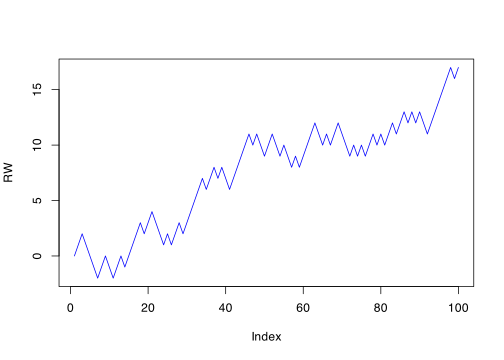
\includegraphics[keepaspectratio]{index_files/mediabag/lectures/L17-markov-intro_files/figure-pdf/rw1-1.pdf}}

which goes up on average. With \(p = 0.3\), we have

\begin{Shaded}
\begin{Highlighting}[]
\NormalTok{RW }\OtherTok{\textless{}{-}} \FunctionTok{rrw}\NormalTok{(}\DecValTok{100}\NormalTok{, }\FloatTok{0.3}\NormalTok{)}
\FunctionTok{plot}\NormalTok{(RW, }\AttributeTok{col =} \StringTok{"blue"}\NormalTok{, }\AttributeTok{type =} \StringTok{"l"}\NormalTok{)}
\end{Highlighting}
\end{Shaded}

\pandocbounded{\includegraphics[keepaspectratio]{index_files/mediabag/lectures/L17-markov-intro_files/figure-pdf/rw2-1.pdf}}

which goes down on average. The simple symmetric random walk, with
\(p = 0.5\) can be much more unpredictable.

\begin{Shaded}
\begin{Highlighting}[]
\NormalTok{RW }\OtherTok{\textless{}{-}} \FunctionTok{rrw}\NormalTok{(}\DecValTok{1000}\NormalTok{, }\FloatTok{0.5}\NormalTok{)}
\FunctionTok{plot}\NormalTok{(RW, }\AttributeTok{col =} \StringTok{"black"}\NormalTok{, }\AttributeTok{type =} \StringTok{"l"}\NormalTok{, }\AttributeTok{ylim =} \FunctionTok{c}\NormalTok{(}\SpecialCharTok{{-}}\DecValTok{80}\NormalTok{, }\DecValTok{80}\NormalTok{))}

\NormalTok{cols }\OtherTok{\textless{}{-}} \FunctionTok{c}\NormalTok{(}\StringTok{"red"}\NormalTok{, }\StringTok{"orange"}\NormalTok{, }\StringTok{"yellow"}\NormalTok{, }\StringTok{"green"}\NormalTok{, }\StringTok{"blue"}\NormalTok{, }\StringTok{"darkblue"}\NormalTok{, }\StringTok{"purple"}\NormalTok{)}
\ControlFlowTok{for}\NormalTok{ (i }\ControlFlowTok{in} \DecValTok{1}\SpecialCharTok{:}\DecValTok{7}\NormalTok{) \{}
\NormalTok{  RW }\OtherTok{\textless{}{-}} \FunctionTok{rrw}\NormalTok{(}\DecValTok{1000}\NormalTok{, }\FloatTok{0.5}\NormalTok{)}
  \FunctionTok{points}\NormalTok{(RW, }\AttributeTok{col =}\NormalTok{ cols[i], }\AttributeTok{type =} \StringTok{"l"}\NormalTok{)}
\NormalTok{\}}
\end{Highlighting}
\end{Shaded}

\pandocbounded{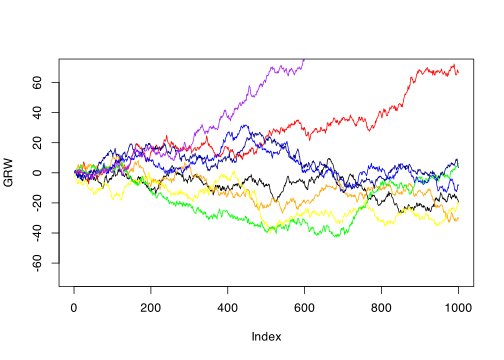
\includegraphics[keepaspectratio]{index_files/mediabag/lectures/L17-markov-intro_files/figure-pdf/ssrw-1.pdf}}

\end{example}

\textbf{Next time.} \emph{We continue our whistle-stop tour of
discrete-space Markov chains.}

\textbf{Summary:}

\begin{itemize}
\item
  A Markov chain is a stochastic process where the next step \(X_{i+1}\)
  depends on the current step \(X_i\), but, given current step
  \(X_{i}\), does not depend on the past \(X_1, \dots, X_{i-1}\).
\item
  A Markov chain is governed by its transition probabilities
  \(p(x, y) = \mathbb P(X_{i+1} = y \mid X_i = x)\). These are written
  in the transition matrix \(\mathsf P\), whose rows add up to 1.
\item
  The simple random walk on the integers at each step goes up 1 with
  probability \(p\) and down 1 with probability \(q\). If
  \(p = q = \tfrac12\), it is a simple symmetric random walk.
\end{itemize}

\textbf{Read more:}

\begin{itemize}
\item
  \href{https://leeds.primo.exlibrisgroup.com/permalink/44LEE_INST/1fj430b/cdi_askewsholts_vlebooks_9781118728031}{Voss,
  \emph{An Introduction to Statistical Computing}}, Subsections 2.3.1
\item
  my notes for \href{https://mpaldridge.github.io/math2750/}{MATH2750
  Introduction to Markov Processes}, Lectures 1, 2 and 5.
\end{itemize}

\chapter{Markov chains in the long
run}\label{markov-chains-in-the-long-run}

\section{\texorpdfstring{\emph{n}-step transition
probabilities}{n-step transition probabilities}}\label{n-step-transition-probabilities}

Last time we saw that the probability of a ``1-step transition'' from
\(x\) to \(y\) is
\[ p(x, y) = \mathbb P(X_{i+1} = y \mid X_{i} = x)  .\] But what is the
probability of a ``2-step transition''
\[ p^{(2)}(x, y) = \mathbb P(X_{i+2} = y \mid X_{i} = x) ?\]

Well, the first step will be from \(x\) to some other state \(z\); then
the second step will have to go from that \(z\) to \(y\). Thus we have
\begin{align}
p^{(2)}(x, y) &= \mathbb P(X_{i+2} = y \mid X_{i} = x) \\
&= \sum_{z \in \mathcal S} \mathbb P(X_{i+1} = z \mid X_{i} = x) \,\mathbb P(X_{i+2} = y \mid X_{i+1} = z , X_{i} = x) \\
&= \sum_{z \in \mathcal S} \mathbb P(X_{i+1} = z \mid X_{i} = x) \,\mathbb P(X_{i+2} = y \mid X_{i+1} = z) \\
&= \sum_{z \in \mathcal S} p(x, z)\,p(z, y) .
\end{align} Here, in the third line we used the Markov property to
delete the unnecessary conditioning on \(X_i\).

What we have here, though, is the \((x, y)\)th entry of the matrix
square \(\mathsf P^2 = \mathsf{P}\,\mathsf{P}\). That is, to get the
matrix of 2-step transitions, we simply take the second matrix power of
the matrix of 1-step transitions.

In the same way we can calculate an \(n\)-step transition probability
\(p^{(n)}(x, y) = \mathbb P(X_{i+n} = y \mid X_i = x)\) by summing over
all the potential paths \(x \to z_1 \to \cdots \to z_{n-1} \to y\) of
length \(n\) from \(x\) to \(y\). This gives
\[ p^{(n)}(x, y) = \sum_{z_1, \dots, z_{n-1} \in \mathcal S} p(x, z_1)\,p(z_1, z_2)\cdots p(z_{n-2},z_{n-1})\,p(z_{n-1}, y).\]
This is the expression for the \((x,y)\)th entry of the \(n\)th matrix
power
\(\mathsf{P}^{n} = \mathsf{P}\,\mathsf{P}^{n-1}= \mathsf{P}^{n-1}\,\mathsf{P}\),
so we can find all the \(n\)-step transition probabilities from
\(\mathsf P^n\).

(Remember that the matrix power \(\mathsf P^n\) is what we get by
multiplying the whole matrix \(\mathsf P\) by itself \(n\) times, using
the rules for multiplying matrices. It's not just what we get from
taking the \(n\)th power of the number in each entry. In R, proper
matrix multiplication is \texttt{P\ \%*\%\ P}, while \texttt{P\ *\ P} is
simply entry-wise multiplication.)

\begin{example}[]\protect\hypertarget{exm-2state-nstep}{}\label{exm-2state-nstep}

Let's go back to our two-state ``unreliable printer'' Markov chain.
Here, we had
\[ \mathsf P = \begin{pmatrix} 0.9 & 0.1 \\ 0.5 & 0.5 \end{pmatrix} . \]
The 2-step transition probabilities are given by
\[ \mathsf P^2 = \begin{pmatrix} 0.9 & 0.1 \\ 0.5 & 0.5 \end{pmatrix}\begin{pmatrix} 0.9 & 0.1 \\ 0.5 & 0.5 \end{pmatrix} = \begin{pmatrix} 0.86 & 0.14 \\ 0.7 & 0.3 \end{pmatrix} . \]
So if the printer is working today, there's an 86\% probability it's
working in two days' time, for example.

For bigger matrix powers, it's best to use a computer. In R, the
following ``quick and dirty'' function works well for small powers. (For
larger powers, I recommend finding a package with an appropriate
built-in matrix power function.)

\begin{Shaded}
\begin{Highlighting}[]
\NormalTok{matrixpow }\OtherTok{\textless{}{-}} \ControlFlowTok{function}\NormalTok{(M, n) \{}
  \ControlFlowTok{if}\NormalTok{ (n }\SpecialCharTok{==} \DecValTok{1}\NormalTok{) }\FunctionTok{return}\NormalTok{(M)}
  \ControlFlowTok{else} \FunctionTok{return}\NormalTok{(M }\SpecialCharTok{\%*\%} \FunctionTok{matrixpow}\NormalTok{(M, n }\SpecialCharTok{{-}} \DecValTok{1}\NormalTok{))}
\NormalTok{\}}
\end{Highlighting}
\end{Shaded}

From this we find the 10-step transition probability
\[ \mathsf P^{10} = \begin{pmatrix} 0.8334 & 0.1667 \\ 0.8332 & 0.1668 \end{pmatrix}. \]
The first row of this matrix denotes the probabilities of where we end
up after 10 steps if we start in state 1, and the second row for if we
start in state 2. These are very nearly the same -- we have a
probability \(\approx 0.883\) if being in state 1 and \(\approx 0.167\)
of being in state 2, \emph{regardless of which state we started in}.
It's as if the Markov chain has forgotten where we started.

Similarly, if we look at the 11-step transition probability, that comes
out as
\[ \mathsf P^{11} = \begin{pmatrix} 0.8333 & 0.1667 \\ 0.8333 & 0.1667 \end{pmatrix}, \]
which is virtually the same distribution as after 10 steps. It seems
that, after a large number of steps \(i\), that we are ``settling down''
to a ``long run distribution'' where \(\mathbb P(X_i = 1) = 0.8333\) and
\(\mathbb P(X_i = 2) = 0.1667\), not only regardless of which state we
started in but also for all large \(i\).

\end{example}

We will investigate these phenomena in the next section.

\section{Stationary distributions}\label{stationary-distributions}

Suppose our Markov chain is currently in the distribution \(\pi\) at
step \(i\). That is, for each \(x \in \mathcal S\), we have
\(\mathbb P(X_i = x) = \pi(x)\). What is the probability we are in state
\(y\) at the next step \(i+1\)? Well, conditioning on the current step,
we have
\[ \mathbb P(X_{i+1} = y) = \sum_{x \in \mathcal S} \mathbb P(X_i = x) \,\mathbb P(X_{i+1} = y \mid X_i = x) = \sum_{x \in \mathcal S} \pi(x) \,p(x, y) . \]

Now if, \(X_{i+1}\) \emph{also} has the distribution \(\pi\) -- that is,
if \(\mathbb P(X_{i+1} = y) = \pi(y)\) -- then we would remain in the
distribution \(\pi\) a time step \(i+1\). And, by the same logic, time
steps \(i+2, i+3, \dots\) and forever. That seems a bit like what we saw
happening in Example~\ref{exm-2state-nstep}. We call this a
\textbf{stationary distribution}.

A stationary distribution means that \emph{the probability of being in
state \(x\)} is staying the same, as \(\pi(x)\). Any particular
realisation of the Markov chain will, of course, continue moving between
states.

\begin{definition}[]\protect\hypertarget{def-statdist}{}\label{def-statdist}

Let \((X_i)\) be a Markov chain on a discrete state space \(\mathcal S\)
with transition matrix \(\mathsf P = (p(x,y))\). Let \(\pi\) be a
distribution on \(\mathcal S\), in that \(\pi(x) \geq 0\) for all \(x\)
and \(\sum_{x \in \mathcal S} \pi(x) = 1\). If, for all
\(y \in \mathcal S\) we have
\begin{equation}\phantomsection\label{eq-statdist}{ \pi(y) = \sum_{x \in \mathcal S} \pi(x) \,p(x, y) , }\end{equation}
then we say that \(\pi\) is a \textbf{stationary distribution}.

\end{definition}

In matrix form, we can write Equation~\ref{eq-statdist} as
\(\boldsymbol\pi = \boldsymbol\pi\mathsf P\), where \(\boldsymbol\pi\)
is a \emph{row} vector (not the more common column vector holding the
values of \(\pi(x)\).

Solving Equation~\ref{eq-statdist} or
\(\boldsymbol\pi = \boldsymbol\pi\mathsf P\) can be a bit fiddly. It's
often easier to check something called the \textbf{detailed balance
equations}.

\begin{theorem}[]\protect\hypertarget{thm-detbal}{}\label{thm-detbal}

Let \((X_i)\) be a Markov chain on a discrete state space \(\mathcal S\)
with transition matrix \(\mathsf P = (p(x,y))\). Let \(\pi\) be a
distribution on \(\mathcal S\) that solved the \textbf{detailed balance
equations}
\[ \pi(y) \,p(y, x) = \pi(x)\,p(x,y) \qquad \text{for all $x, y \in \mathcal S$.} \]
Then \(\pi\) is a stationary distribution.

\end{theorem}

\begin{proof}
Sum both sides over \(x\). The left-hand side becomes
\[ \sum_{x \in \mathcal S} \pi(y)\,p(y,x) = \pi(y) \sum_{x \in \mathcal S} p(y,x) = \pi(y) , \]
since rows of a transition matrix sum up to 1. The right hand side
becomes \[ \sum_{x \in \mathcal S}\pi(x)\,p(x,y) .\] Hence, we have
\[ \pi(y) = \sum_{x \in \mathcal S} \pi(x) \,p(x, y) , \] which is the
definition of a stationary distribution.
\end{proof}

\begin{example}[]\protect\hypertarget{exm-2state-stat}{}\label{exm-2state-stat}

We return to Example~\ref{exm-2state} and
Example~\ref{exm-2state-nstep}. There's no need to check the detailed
balance equations when \(x = y\), so we just need
\[ \pi(2)\,p(2, 1) = \pi(1)\,p(1, 2) \qquad \Longrightarrow \qquad 0.5\pi(2) = 0.1\pi(1) .\]
Remembering that \(\pi\) must sum to 1, we get
\(\pi(1) = \tfrac16 = 0.1667\) and \(\pi(2) = \tfrac56 = 0.8333\).

Look how that compares with our results for \(\mathsf P^{10}\) and
\(\mathsf P^{11}\) -- this \(\pi\) was precisely the values we saw in
every row of \(\mathsf P^n\) for large \(n\).

\end{example}

\section{Limit theorems}\label{limit-theorems}

The big central theorem of Markov chains in discrete space is the
following. We will highlight some technical conditions in {red} that we
will return to later.

\begin{theorem}[]\protect\hypertarget{thm-ergodic}{}\label{thm-ergodic}

Let \((X_i)\) be a Markov chain on a discrete state space \(\mathcal S\)
with transition matrix \(\mathsf P\). Suppose that \((X_i)\) is
{irreducible} and {positive recurrent}.

\begin{enumerate}
\def\labelenumi{\arabic{enumi}.}
\item
  There exists a stationary distribution \(\pi\), which is unique.
\item
  \textbf{(Limit theorem)} If \((X_i)\) is also {aperiodic}, then
  \(\mathbb P(X_n = y \mid X_1 = x) \to \pi(y)\) as \(n \to \infty\) for
  all \(y \in \mathcal S\) , regardless of the starting state
  \(X_1 = x\), where \(\pi\) is the unique stationary distribution.
\item
  \textbf{(Ergodic theorem, 1)} Write
  \[V_n(x) = \frac{1}{n} \big|\{i = 1, 2, \dots, n : X_i = x\}\big|\]
  for the proportion of the first \(n\) steps spent in state \(x\). Then
  \(V_n(x) \to \pi(x)\) as \(n \to \infty\) for all
  \(x \in \mathcal S\), regardless of the starting state \(X_1\), where
  \(\pi\) is the unique stationary distribution.
\item
  \textbf{(Ergodic theorem, 2)} Let \(\phi\) be a function on the state
  space \(\mathcal S\). Let \(X\) have probability mass function
  \(\pi\), where \(\pi\) is the unique stationary distribution. Then
  \[ \frac{1}{n} \sum_{i=1}^n \phi(X_i) \to \operatorname{\mathbb E}\phi(X), \]
  as \(n \to \infty\), regardless of the starting state \(X_1\).
\end{enumerate}

\end{theorem}

(``Ergodic'' is a word mathematicians use when talking about long-run
average behaviour.)

The precise mathematical statements of this theorem are not important
for this module. However, it is important to have a rough idea what the
statements mean -- especially part 4, which is central to the idea of
Markov chain Monte Carlo we will discuss over the next lectures.

The first part tells us that (provided the technical conditions are
fulfilled) we always have a stationary distribution and there's always
exactly one of them. This allows us to use phrases like ``where \(\pi\)
is the unique stationary distribution'' in the other parts of the
theorem.

The second part tells us that any \(n\)-step transition probability
\(p^{(n)}(x,y)\) tends to \(\pi(y)\), no matter what the value of \(x\).
In terms of the \(n\)-step transition matrix \(\mathsf P^n\), this means
that every row of \(\mathsf P^n\) should end up looking like an
identical copy of the row vector \(\boldsymbol\pi\). That is exactly
what we found in Example~\ref{exm-2state-nstep}.

The third part tells us that, in the long run, \(\pi\) describes the
proportion of time we spend in each state. In the ``unreliable printer''
example of Example~\ref{exm-2state-stat}, this means that the printer
spends 83\% of the time working and 17\% of the time broken in the long
run, regardless of whether it was working or broken on day 1.

The fourth part is by far the most important result for us, as it
relates Markov chains back to the idea of Monte Carlo estimation. Let's
look at the equation in the fourth part,
\[ \frac{1}{n} \sum_{i=1}^n \phi(X_i) \to \operatorname{\mathbb E}\phi(X). \]
If the \(X_i\) were independent and identically distributed, this would
just be the ordinary law of large numbers, which tells us that the Monte
Carlo estimator (the left-hand side) is an accurate estimator of
\(\operatorname{\mathbb E}\phi(X)\), when the number of samples is
large. This result tells us that we still get a good estimator when the
\(X_i\) are not IID, but rather come from a Markov chain whose
stationary distribution is the PMF of \(X\).

This fourth part is what allows us to do \textbf{Markov chain Monte
Carlo} (\textbf{MCMC}): Monte Carlo estimation when the \(X_i\) are the
outputs from a Markov chain. If we want to estimate
\(\operatorname{\mathbb E}\phi(X)\), we just need to find a Markov chain
who stationary distribution is the PMF of \(X\), and then form the Monte
Carlo estimate in the usual way. In the next lecture, the
\textbf{Metropolis--Hastings algorithm} will show us a way to do find a
Markov chain with a given stationary distribution.

A quick word before we end about the {technical conditions} in
Theorem~\ref{thm-ergodic}. The precise definitions are not important
here, but let us say the following:

\begin{itemize}
\item
  \textbf{Irreducible} roughly means that a Markov chain is ``connected
  up'', and isn't just two Markov separate Markov chains (for example).
  Specifically, it must be at least \emph{possible} to get from any
  state \(x\) to any other state \(y\) -- maybe not in a single step,
  but in some finite number of steps, with probability greater than 0.
\item
  \textbf{Aperiodic} is another technical condition, but if an
  irreducible Markov chain ever has a non-zero probability of staying in
  the same state, then this is fulfilled. The Markov chains we look at
  for MCMC will all have a strictly positive probability of staying put,
  so will be aperiodic.
\item
  \textbf{Positive recurrence} is a highly technical condition we won't
  get into here.
\end{itemize}

If you do want to read more about the theory of Markov chains, and these
technical conditions in particular, I recommend my lecture notes for my
notes for \href{https://mpaldridge.github.io/math2750/}{MATH2750
Introduction to Markov Processes}. This is entirely optional, though,
and this knowledge is \emph{not} required for this module and its exam.

\textbf{Next time.} \emph{We will look at Markov chain Monte Carlo;
specifically, how to set up a Markov chain that has a given probability
mass function as its stationary distribution.}

\textbf{Summary:}

\begin{itemize}
\item
  The \(n\)-step transition probabilities
  \(p^{(n)}(x,y) = \mathbb{P}(X_{i+n} = y \mid X_i = x)\) can be found
  from the \(n\)th matrix power \(\mathsf P^n\).
\item
  A stationary distribution \(\pi\) for a Markov chain satisfies the
  detailed balance equations \(\pi(y)\,p(y,x) = \pi(x)\,p(x,y)\).
\item
  The ergodic theorem says that (under certain technical conditions)
  \(\frac{1}{n}\sum_{i=1}^n \phi(X_i)\), where \(X_i\) is Markov chain,
  tends to \(\operatorname{\mathbb E}\phi(X)\), where the PMF of \(X\)
  is the unique stationary distribution of the Markov chain.
\end{itemize}

\textbf{Read more:}

\begin{itemize}
\item
  \href{https://leeds.primo.exlibrisgroup.com/permalink/44LEE_INST/1fj430b/cdi_askewsholts_vlebooks_9781118728031}{Voss,
  \emph{An Introduction to Statistical Computing}}, Subsections 2.3.1
  and 4.1.2
\item
  my notes for \href{https://mpaldridge.github.io/math2750/}{MATH2750
  Introduction to Markov Processes}, Lectures 7 and 9--11
\end{itemize}

\chapter{Metropolis--Hastings in discrete
space}\label{metropolishastings-in-discrete-space}

\section{The Metropolis--Hastings
algorithm}\label{the-metropolishastings-algorithm}

Last time, we looked at the long-run behaviour of a Markov chain
\((X_i)\). We saw that (under certain technical conditions) the Markov
chain has a unique stationary distribution \(\pi\), which we can find by
solving the detailed balance equations
\(\pi(y)\,p(y,x) = \pi(x)\,p(x,y)\).

We then saw the ergodic theorem: If \(\phi\) be a function on the state
space \(\mathcal S\) and \(X\) has probability mass function \(\pi\),
then
\[ \frac{1}{n} \sum_{i=1}^n \phi(X_i) \to \operatorname{\mathbb E}\phi(X), \]
as \(n \to \infty\). This means we can do Monte Carlo estimation where
the samples \(X_1, \dots, X_n\) are not IID, but are rather the output
to a Markov chain with stationary distribution \(\pi\).

So, suppose we want to estimate \(\operatorname{\mathbb E} \phi(X)\),
where \(X\) has PDF \(\pi\). Then all we need to find a Markov chain
that has \(\pi\) as its stationary distribution. We could try to do that
be being clever -- just by thinking hard and trying to come up with one.
However, that's rather difficult. Instead, the
\textbf{Metropolis--Hastings algorithm} is a method to create such a
Markov chain.

The Metropolis--Hastings algorithm is based on a similar idea to
rejection sampling. From state \(X_i = x\), we \emph{propose} moving to
some other state \(y\), and then we accept the proposal with some
acceptance probability. If we accept the proposal, we move to
\(X_{i+1} = y\); if we reject the proposal, we stay where we are
\(X_{i+1} = x\).

\href{https://en.wikipedia.org/wiki/Nicholas_Metropolis}{Nicholas
Metropolis} first came up with this idea when he worked with Ulam and
von Neumann (of Monte Carlo fame) at the Los Alamos National
Laboratories. His original idea was generalised by the Canadian
statistician WK Hastings.

The Metropolis--Hastings algorithm works like this:

\begin{itemize}
\item
  We want to define a Markov chain on a state space \(\mathcal S\),
  which contains the range of the probability mass function \(\pi\) we
  want to sample from.
\item
  We have an initial state \(X_1 = x_1\) and we choose a transition
  matrix \(\mathsf R = (r(x,y))\) representing the proposal moves.
\end{itemize}

\begin{enumerate}
\def\labelenumi{\arabic{enumi}.}
\item
  From a current state \(X_i = x\) we propose moving to a new state
  \(y\), where \(y\) is chosen with probability \(r(x, y)\).
\item
  With probability
  \[\alpha(x,y) = \min \left\{ \frac{\pi(y)\,r(y,x)}{\pi(x)\,r(x,y)} , \, 1\right\} , \]
  we accept the proposal, and set \(X_i = y\); otherwise we stay put,
  and set \(X_{i+1} = x\).
\item
  We repeat steps 1. and 2. \(n\) times to get \(n\) samples.
\end{enumerate}

So a generic Metropolis--Hastings algorithm on a finite state space in
``sort-of-R-code'' would look something like this:

\begin{Shaded}
\begin{Highlighting}[]
\CommentTok{\# INPUTS:}
\CommentTok{\# trans:   proposal transition matrix}
\CommentTok{\# target:  target stationary distribution}
\CommentTok{\# initial: initial state}
\CommentTok{\# n:       number of samples}

\NormalTok{states }\OtherTok{\textless{}{-}} \FunctionTok{nrow}\NormalTok{(trans)}
\NormalTok{MC }\OtherTok{\textless{}{-}} \FunctionTok{rep}\NormalTok{(}\DecValTok{0}\NormalTok{, n)}
\NormalTok{accept }\OtherTok{\textless{}{-}} \ControlFlowTok{function}\NormalTok{(x, y) \{}
\NormalTok{  ratio }\OtherTok{\textless{}{-}}\NormalTok{ (target[y] }\SpecialCharTok{*}\NormalTok{ trans[y, x]) }\SpecialCharTok{/}\NormalTok{ (target[x] }\SpecialCharTok{*}\NormalTok{ trans[x, y])}
  \FunctionTok{min}\NormalTok{(ratio, }\DecValTok{1}\NormalTok{)}
\NormalTok{\}}

\NormalTok{MC[}\DecValTok{1}\NormalTok{] }\OtherTok{\textless{}{-}}\NormalTok{ initial}
\ControlFlowTok{for}\NormalTok{ (i }\ControlFlowTok{in} \DecValTok{1}\SpecialCharTok{:}\NormalTok{(n }\SpecialCharTok{{-}} \DecValTok{1}\NormalTok{)) \{}
\NormalTok{  prop }\OtherTok{\textless{}{-}} \FunctionTok{sample}\NormalTok{(}\DecValTok{1}\SpecialCharTok{:}\NormalTok{states, }\DecValTok{1}\NormalTok{, }\AttributeTok{prob =}\NormalTok{ trans[MC[i], ])}
  \ControlFlowTok{if}\NormalTok{ (}\FunctionTok{runif}\NormalTok{(}\DecValTok{1}\NormalTok{) }\SpecialCharTok{\textless{}=} \FunctionTok{accept}\NormalTok{(MC[i], prop)) MC[i }\SpecialCharTok{+} \DecValTok{1}\NormalTok{] }\OtherTok{\textless{}{-}}\NormalTok{ prop}
  \ControlFlowTok{else}\NormalTok{                                 MC[i }\SpecialCharTok{+} \DecValTok{1}\NormalTok{] }\OtherTok{\textless{}{-}}\NormalTok{ MC[i]}
\NormalTok{\}}
\end{Highlighting}
\end{Shaded}

It's the last three lines that are important here. In this code
\texttt{MC} records the states of our Markov chain. First we propose a
move to state \texttt{prop}, according to the row of the transition
matrix corresponding to the current state. Second, we accept that
proposal move with probability \texttt{accept()}, where the arguments of
\texttt{accept()} are the current state and the proposed state; we do
this by checking whether a standard uniform \texttt{runif(1)} is less
than this acceptance probability or not. If it is, we move to
\texttt{prop} (last-but-one line); and if not, we stay where we are
(last line).

We will show later that this algorithm really does have \(\pi\) as its
stationary distribution.

\section{Random walk Metropolis}\label{random-walk-metropolis}

There are quite a lot of cases where the proposals are
\textbf{symmetric}, meaning that \(r(x, y) = r(y, x)\). This is the case
if, for example, the proposal probabilities are those of the simple
symmetric random walk: \(r(x, x+1) = \frac12\) and
\(r(x, x-1) = \frac12\). In the symmetric case, the acceptance
probability simplifies to
\[ \alpha(x, y) = \min \left\{ \frac{\pi(y)}{\pi(x)} , \, 1\right\} . \]

The symmetric case was the version originally considered by Metropolis,
before Hastings generalised it to non-symmetric proposals. For this
reasons, when \(\mathsf R\) has this symmetry property, we often refer
to the resulting algorithm just as the \textbf{Metropolis algorithm}.
When the proposal probabilities are those of the simple symmetric random
walk, we call it the \textbf{random walk Metropolis algorithm}.

\begin{example}[]\protect\hypertarget{exm-MCMC-geom}{}\label{exm-MCMC-geom}

Let's do an example of the random walk Metropolis algorithm where we aim
to sample from the geometric distribution with parameter \(\frac13\),
\[ \pi(x) = \Big(\frac23\Big)^{x-1}\times \frac13 \qquad x = 1, 2, \dots. \]
We will start from \(X_1 = 1\).

So at each step we propose moving up one with probability \(\tfrac12\)
and moving down one with probability \(\tfrac12\). Since the proposals
are symmetric, the acceptance probabilities are \[ \begin{align}
\alpha(x, x+1) = \min \left\{ \frac{\pi(x+1)}{\pi(x)} , \, 1\right\} = \min \left\{\frac{\big(\frac23\big)^{x}\times \frac13}{\big(\frac23\big)^{x-1}\times \frac13},\, 1\right\} = \min \Big\{\frac23, 1\Big\} = \frac23 \\
\alpha(x, x-1) = \min \left\{ \frac{\pi(x-1)}{\pi(x)} , \, 1\right\} = \min \left\{\frac{\big(\frac23\big)^{x-1}\times \frac13}{\big(\frac23\big)^{x}\times \frac13},\, 1\right\} = \min \Big\{\frac32, 1\Big\} = 1 , 
\end{align} \] except for
\[\alpha(1, 0) = \min \left\{ \frac{\pi(0)}{\pi(1)} , \, 1\right\} = \min \left\{ \frac{0}{\frac13} , \, 1\right\} = \min \{0,1\} = 0 .\]
So if the proposal is up one, we accept it with probability \(\frac23\)
and otherwise stay where we are. If the proposal is down one, we always
accept -- except going down from 1 to 0, which we always reject.

Let's try it.

\begin{Shaded}
\begin{Highlighting}[]
\NormalTok{n }\OtherTok{\textless{}{-}} \FloatTok{1e6}
\NormalTok{MC }\OtherTok{\textless{}{-}} \FunctionTok{rep}\NormalTok{(}\DecValTok{0}\NormalTok{, n)}

\NormalTok{MC[}\DecValTok{1}\NormalTok{] }\OtherTok{\textless{}{-}} \DecValTok{1}
\ControlFlowTok{for}\NormalTok{ (i }\ControlFlowTok{in} \DecValTok{1}\SpecialCharTok{:}\NormalTok{(n }\SpecialCharTok{{-}} \DecValTok{1}\NormalTok{)) \{}
\NormalTok{  prop }\OtherTok{\textless{}{-}}\NormalTok{ MC[i] }\SpecialCharTok{+} \FunctionTok{sample}\NormalTok{(}\FunctionTok{c}\NormalTok{(}\SpecialCharTok{+}\DecValTok{1}\NormalTok{, }\SpecialCharTok{{-}}\DecValTok{1}\NormalTok{), }\DecValTok{1}\NormalTok{, }\AttributeTok{prob =} \FunctionTok{c}\NormalTok{(}\DecValTok{1}\SpecialCharTok{/}\DecValTok{2}\NormalTok{, }\DecValTok{1}\SpecialCharTok{/}\DecValTok{2}\NormalTok{))}
  \ControlFlowTok{if}\NormalTok{      (prop }\SpecialCharTok{==} \DecValTok{0}\NormalTok{)         MC[i }\SpecialCharTok{+} \DecValTok{1}\NormalTok{] }\OtherTok{\textless{}{-}}\NormalTok{ MC[i]}
  \ControlFlowTok{else} \ControlFlowTok{if}\NormalTok{ (prop }\SpecialCharTok{==}\NormalTok{ MC[i] }\SpecialCharTok{{-}} \DecValTok{1}\NormalTok{) MC[i }\SpecialCharTok{+} \DecValTok{1}\NormalTok{] }\OtherTok{\textless{}{-}}\NormalTok{ MC[i] }\SpecialCharTok{{-}} \DecValTok{1}
  \ControlFlowTok{else} \ControlFlowTok{if}\NormalTok{ (prop }\SpecialCharTok{==}\NormalTok{ MC[i] }\SpecialCharTok{+} \DecValTok{1}\NormalTok{) MC[i }\SpecialCharTok{+} \DecValTok{1}\NormalTok{] }\OtherTok{\textless{}{-}}\NormalTok{ MC[i] }\SpecialCharTok{+}\NormalTok{ (}\FunctionTok{runif}\NormalTok{(}\DecValTok{1}\NormalTok{) }\SpecialCharTok{\textless{}=} \DecValTok{2}\SpecialCharTok{/}\DecValTok{3}\NormalTok{)}
\NormalTok{\}}
\end{Highlighting}
\end{Shaded}

If we look at a graph of the first 250 steps of this Markov chain, we
see that these aren't at all random samples from the geometric
distribution -- each step is either the same as the one before, one
bigger, or one smaller.

\begin{Shaded}
\begin{Highlighting}[]
\FunctionTok{plot}\NormalTok{(}
\NormalTok{  MC[}\DecValTok{1}\SpecialCharTok{:}\DecValTok{250}\NormalTok{],}
  \AttributeTok{type =} \StringTok{"l"}\NormalTok{, }\AttributeTok{col =} \StringTok{"red"}\NormalTok{, }\AttributeTok{lwd =} \DecValTok{2}\NormalTok{,}
  \AttributeTok{xlab =} \StringTok{"time step"}\NormalTok{, }\AttributeTok{ylab =} \StringTok{"value"}
\NormalTok{)}
\end{Highlighting}
\end{Shaded}

\pandocbounded{\includegraphics[keepaspectratio]{index_files/mediabag/lectures/L19-mh-1_files/figure-pdf/MCgeom1-1.pdf}}

But if we look at a graph of which samples came up overall, we see that
their proportions (red) are extremely close to what we would expect from
the true geometric distribution (blue).

\begin{Shaded}
\begin{Highlighting}[]
\FunctionTok{plot}\NormalTok{(}
  \FunctionTok{table}\NormalTok{(MC)}\SpecialCharTok{/}\NormalTok{n,}
  \AttributeTok{xlim =} \FunctionTok{c}\NormalTok{(}\DecValTok{0}\NormalTok{, }\DecValTok{10}\NormalTok{), }\AttributeTok{col =} \StringTok{"red"}\NormalTok{, }\AttributeTok{ylim =} \FunctionTok{c}\NormalTok{(}\DecValTok{0}\NormalTok{, }\FloatTok{0.35}\NormalTok{), }\AttributeTok{lwd =} \DecValTok{2}\NormalTok{,}
  \AttributeTok{xlab =} \StringTok{"value"}\NormalTok{, }\AttributeTok{ylab =} \StringTok{"probability"}
\NormalTok{)}

\FunctionTok{points}\NormalTok{(}\DecValTok{1}\SpecialCharTok{:}\DecValTok{10} \SpecialCharTok{+} \FloatTok{0.1}\NormalTok{, (}\DecValTok{2}\SpecialCharTok{/}\DecValTok{3}\NormalTok{)}\SpecialCharTok{\^{}}\NormalTok{(}\DecValTok{1}\SpecialCharTok{:}\DecValTok{10} \SpecialCharTok{{-}} \DecValTok{1}\NormalTok{) }\SpecialCharTok{*}\NormalTok{ (}\DecValTok{1}\SpecialCharTok{/}\DecValTok{3}\NormalTok{), }\AttributeTok{col =} \StringTok{"blue"}\NormalTok{, }\AttributeTok{type =} \StringTok{"h"}\NormalTok{, }\AttributeTok{lwd =} \DecValTok{3}\NormalTok{)}

\FunctionTok{legend}\NormalTok{(}\StringTok{"topright"}\NormalTok{, }\FunctionTok{c}\NormalTok{(}\StringTok{"samples"}\NormalTok{, }\StringTok{"true geometric"}\NormalTok{),}
  \AttributeTok{col =} \FunctionTok{c}\NormalTok{(}\StringTok{"red"}\NormalTok{, }\StringTok{"blue"}\NormalTok{), }\AttributeTok{lwd =} \FunctionTok{c}\NormalTok{(}\DecValTok{2}\NormalTok{, }\DecValTok{3}\NormalTok{)}
\NormalTok{)}
\end{Highlighting}
\end{Shaded}

\pandocbounded{\includegraphics[keepaspectratio]{index_files/mediabag/lectures/L19-mh-1_files/figure-pdf/MCgeom-1.pdf}}

Suppose we wanted to estimate \(\mathbb EX^2\), where
\(X \sim \operatorname{Geom}(\frac{1}{3})\). We already know how to do
this the ``basic'' Monte Carlo way. But we can now do it the Markov
chain Monte Carlo (MCMC) way, by using the output to this Markov chain.

Our estimate is the following.

\begin{Shaded}
\begin{Highlighting}[]
\FunctionTok{mean}\NormalTok{(MC}\SpecialCharTok{\^{}}\DecValTok{2}\NormalTok{) }
\end{Highlighting}
\end{Shaded}

\begin{verbatim}
[1] 14.79205
\end{verbatim}

The true answer is 15, so we are in the right area, but probably not as
accurate as the basic Monte Carlo estimator with the same sample size
would have been. This suggests that the dependence structure in a Markov
chain might be a slight disadvantage, and may make the variance of our
estimator bigger. The real strength of MCMC is when a basic Monte Carlo
estimate is impossible to get -- when basic MCMC is possible (such as
for simple distributions like this geometric) we should probably stick
with it.

\end{example}

\section{Proof of stationary
distribution}\label{proof-of-stationary-distribution}

We have defined the Metropolis--Hastings Markov chain in terms of the
proposal transition probabilities \(r(x, y)\) and the acceptance
probability \(\alpha(x, y)\). But what are the actual transition
probability \(p(x, y)\) of this Markov chain?

Well, to move from \(x\) to \(y \neq x\), we first have to propose that
move, then we have to accept it. So we have
\begin{equation}\phantomsection\label{eq-MHp}{ p(x, y) = r(x, y) \,\alpha(x, y) = r(x, y) \,\min \left\{ \frac{\pi(y)\,r(y,x)}{\pi(x)\,r(x,y)} , \, 1\right\} .}\end{equation}
(We can find \(p(x,x)\), if we need it, by using the fact that
\(\sum_y p(x,y) = 0\).)

We should check that the Metropolis--Hastings algorithm really does give
a Markov chain with stationary distribution \(\pi\).

\begin{theorem}[]\protect\hypertarget{thm-MHpi}{}\label{thm-MHpi}

Let \(\pi\) be a probability mass function on a discrete state space
\(\mathcal S\), and let \(\mathsf R = (r(x,y))\) be a transition matrix
on \(\mathcal S\). Let \((X_i)\) be the Metropolis--Hastings Markov
chain with proposal transition matrix \(\mathsf R\) and acceptance
probability
\[ \alpha(x, y) = \min \left\{ \frac{\pi(y)\,r(y,x)}{\pi(x)\,r(x,y)},\,1\right\} . \]
Then \(\pi\) is a stationary distribution for \((X_i)\).

\end{theorem}

We say ``a'' stationary distribution. But provided the Markov chain
fulfils the technical conditions in Theorem~\ref{thm-ergodic}, we know
that this will be the unique stationary distribution, and that the
ergodic theorem will hold.

\begin{proof}
We need to check the detailed balance equations
\[ \pi(y) \,p(y, x) = \pi(x) \,p(x, y) \] for \(y \neq x\). By
Equation~\ref{eq-MHp}, the detailed balance equations are
\begin{equation}\phantomsection\label{eq-MHDB}{ \pi(y)\,r(y, x) \,\min \left\{ \frac{\pi(x)\,r(x,y)}{\pi(y)\,r(y,x)} , \, 1\right\} = \pi(x)\,r(x, y) \,\min \left\{ \frac{\pi(y)\,r(y,x)}{\pi(x)\,r(x,y)} , \, 1\right\} . }\end{equation}
Note that the two fractions in the first terms on the minimums are
reciprocals of each other. So one of these will be greater than equal to
1, and the minimum will be 1; and one of the will be less than or equal
to 1, and the minimum will be that fraction.

Suppose first that
\[\frac{\pi(x)\,r(x,y)}{\pi(y)\,r(y,x)} \geq 1 \qquad\text{and} \qquad \frac{\pi(y)\,r(y,x)}{\pi(x)\,r(x,y)} \leq 1 .\]
Then Equation~\ref{eq-MHDB} becomes
\[ \pi(y)\,r(y, x) \times 1 = \pi(x)\,r(x, y) \times \frac{\pi(y)\,r(y,x)}{\pi(x)\,r(x,y)}  . \]
On the right-hand side, the two \(\pi(x)\,r(x,y)\) terms cancel, so we
have equality, and the detailed balance equations hold.

If, on the other hand
\[\frac{\pi(x)\,r(x,y)}{\pi(y)\,r(y,x)} \leq 1 \qquad\text{and} \qquad \frac{\pi(y)\,r(y,x)}{\pi(x)\,r(x,y)} \geq 1 ,\]
then the same argument works the other way around.
\end{proof}

\textbf{Next time.} \emph{We will start our study of MCMC in continuous
space by giving an overview of the theory of Markov chains in continuous
space.}

\textbf{Summary:}

\begin{itemize}
\item
  The Metropolis--Hastings algorithm gives a way of designing a Markov
  chain whose stationary distribution is a given PMF \(\pi\).
\item
  We make proposal moves according to a transition matrix
  \(\mathsf R = (r(x,y))\). A proposal move from \(x\) to \(y\) is
  accepted with probability
  \[\alpha(x,y) = \min \left\{ \frac{\pi(y)\,r(y,x)}{\pi(x)\,r(x,y)} , \, 1\right\} . \]
\item
  The most important example is the random walk Metropolis algorithm,
  where \(`mathsf R\) is the transition matrix of the simple symmetric
  random walk and
  \[\alpha(x,y) = \min \left\{ \frac{\pi(y)}{\pi(x)} , \, 1\right\} . \]
\end{itemize}

\textbf{Read more:}
\href{https://leeds.primo.exlibrisgroup.com/permalink/44LEE_INST/1fj430b/cdi_askewsholts_vlebooks_9781118728031}{Voss,
\emph{An Introduction to Statistical Computing}}, Subsection 4.1.2.

\chapter{Markov chains in continuous
space}\label{markov-chains-in-continuous-space}

\textbf{Next time.} \emph{We will study the Metropolis--Hastings
algorithm in continuous space.}

\textbf{Summary:}

\begin{itemize}
\tightlist
\item
  m
\end{itemize}

\textbf{Read more:}
\href{https://leeds.primo.exlibrisgroup.com/permalink/44LEE_INST/1fj430b/cdi_askewsholts_vlebooks_9781118728031}{Voss,
\emph{An Introduction to Statistical Computing}}, Subsection 2.3.1.

\chapter{Metropolis--Hastings in continuous
space}\label{metropolishastings-in-continuous-space}

\chapter*{Problem Sheet 4}\label{P4}
\addcontentsline{toc}{chapter}{Problem Sheet 4}

\markboth{Problem Sheet 4}{Problem Sheet 4}

This is Problem Sheet 3, which covers material from Lectures 17 to 21.
You should work through all the questions on this problem sheet in
advance of the problems class, which takes place in the lecture of
\textbf{Thursday 27 November}.

This problem sheet is to help you practice material from the module and
to help you check your learning. It is \emph{not} for formal assessment
and does not count towards your module mark.

If you want some brief informal feedback on \textbf{{[}questions TBC{]}}
(marked ★), you should submit your work electronically through
Gradescope via the module's Minerva page by \textbf{1400 on Tuesday 25
November}. (If you hand-write solutions on paper, the easiest way to
scan-and-submit that work is using the Gradescope app on your phone.) I
will return some brief comments on your those two questions by the
problems class on Thursday 27 November. Because this informal feedback,
and not part of the official assessment, I cannot accept late work for
any reason -- but I am always happy to discuss any of your work on any
question in my office hours.

Full solutions will be released on Friday 28 November.

\bookmarksetup{startatroot}

\chapter*{Solutions}\label{solutions}
\addcontentsline{toc}{chapter}{Solutions}

\markboth{Solutions}{Solutions}

\section*{Problem Sheet 1}\label{P1-sols}
\addcontentsline{toc}{section}{Problem Sheet 1}

\markright{Problem Sheet 1}

\section*{Problem Sheet 2}\label{P2-sols}
\addcontentsline{toc}{section}{Problem Sheet 2}

\markright{Problem Sheet 2}

\section*{Problem Sheet 3}\label{P3-sols}
\addcontentsline{toc}{section}{Problem Sheet 3}

\markright{Problem Sheet 3}




\end{document}
